%PDF DI RIFERIMENTO: 04_Modelli di Dominio.pdf, Statecharts.pdf

\chapter{Requirement Specification}
    \section{Obiettivo}
        I requisiti che sono stati riorganizzati nella fase di analisi sono formalizzati in diagrammi (diagramma di classe, diagramma di sequenza, diagramma degli stati) attraverso l'uso di linguaggi di modellazione come UML. \\
        Per individuare il modello ad oggetti per questo dominio, si è scelto di impiegare l'euristica "Three-Object-Type" perché permette di costruire un modello più flessibile e facile da modificare.

    \section{Class Diagram}
        Il Class Diagram individua quali sono le entità coinvolte all'interno del nostro dominio e le relazioni che tra esse sussistono.\\
        In particolare, il modello concettuale basato sull'analisi dei requisiti permetterà di creare un modello efficace per la gestione delle aste.\\
        \subsection{Class Diagram del dominio del problema}
            %Class Diagram costruito con StarUML
            \begin{figure}[htbp!]
                \centering
                    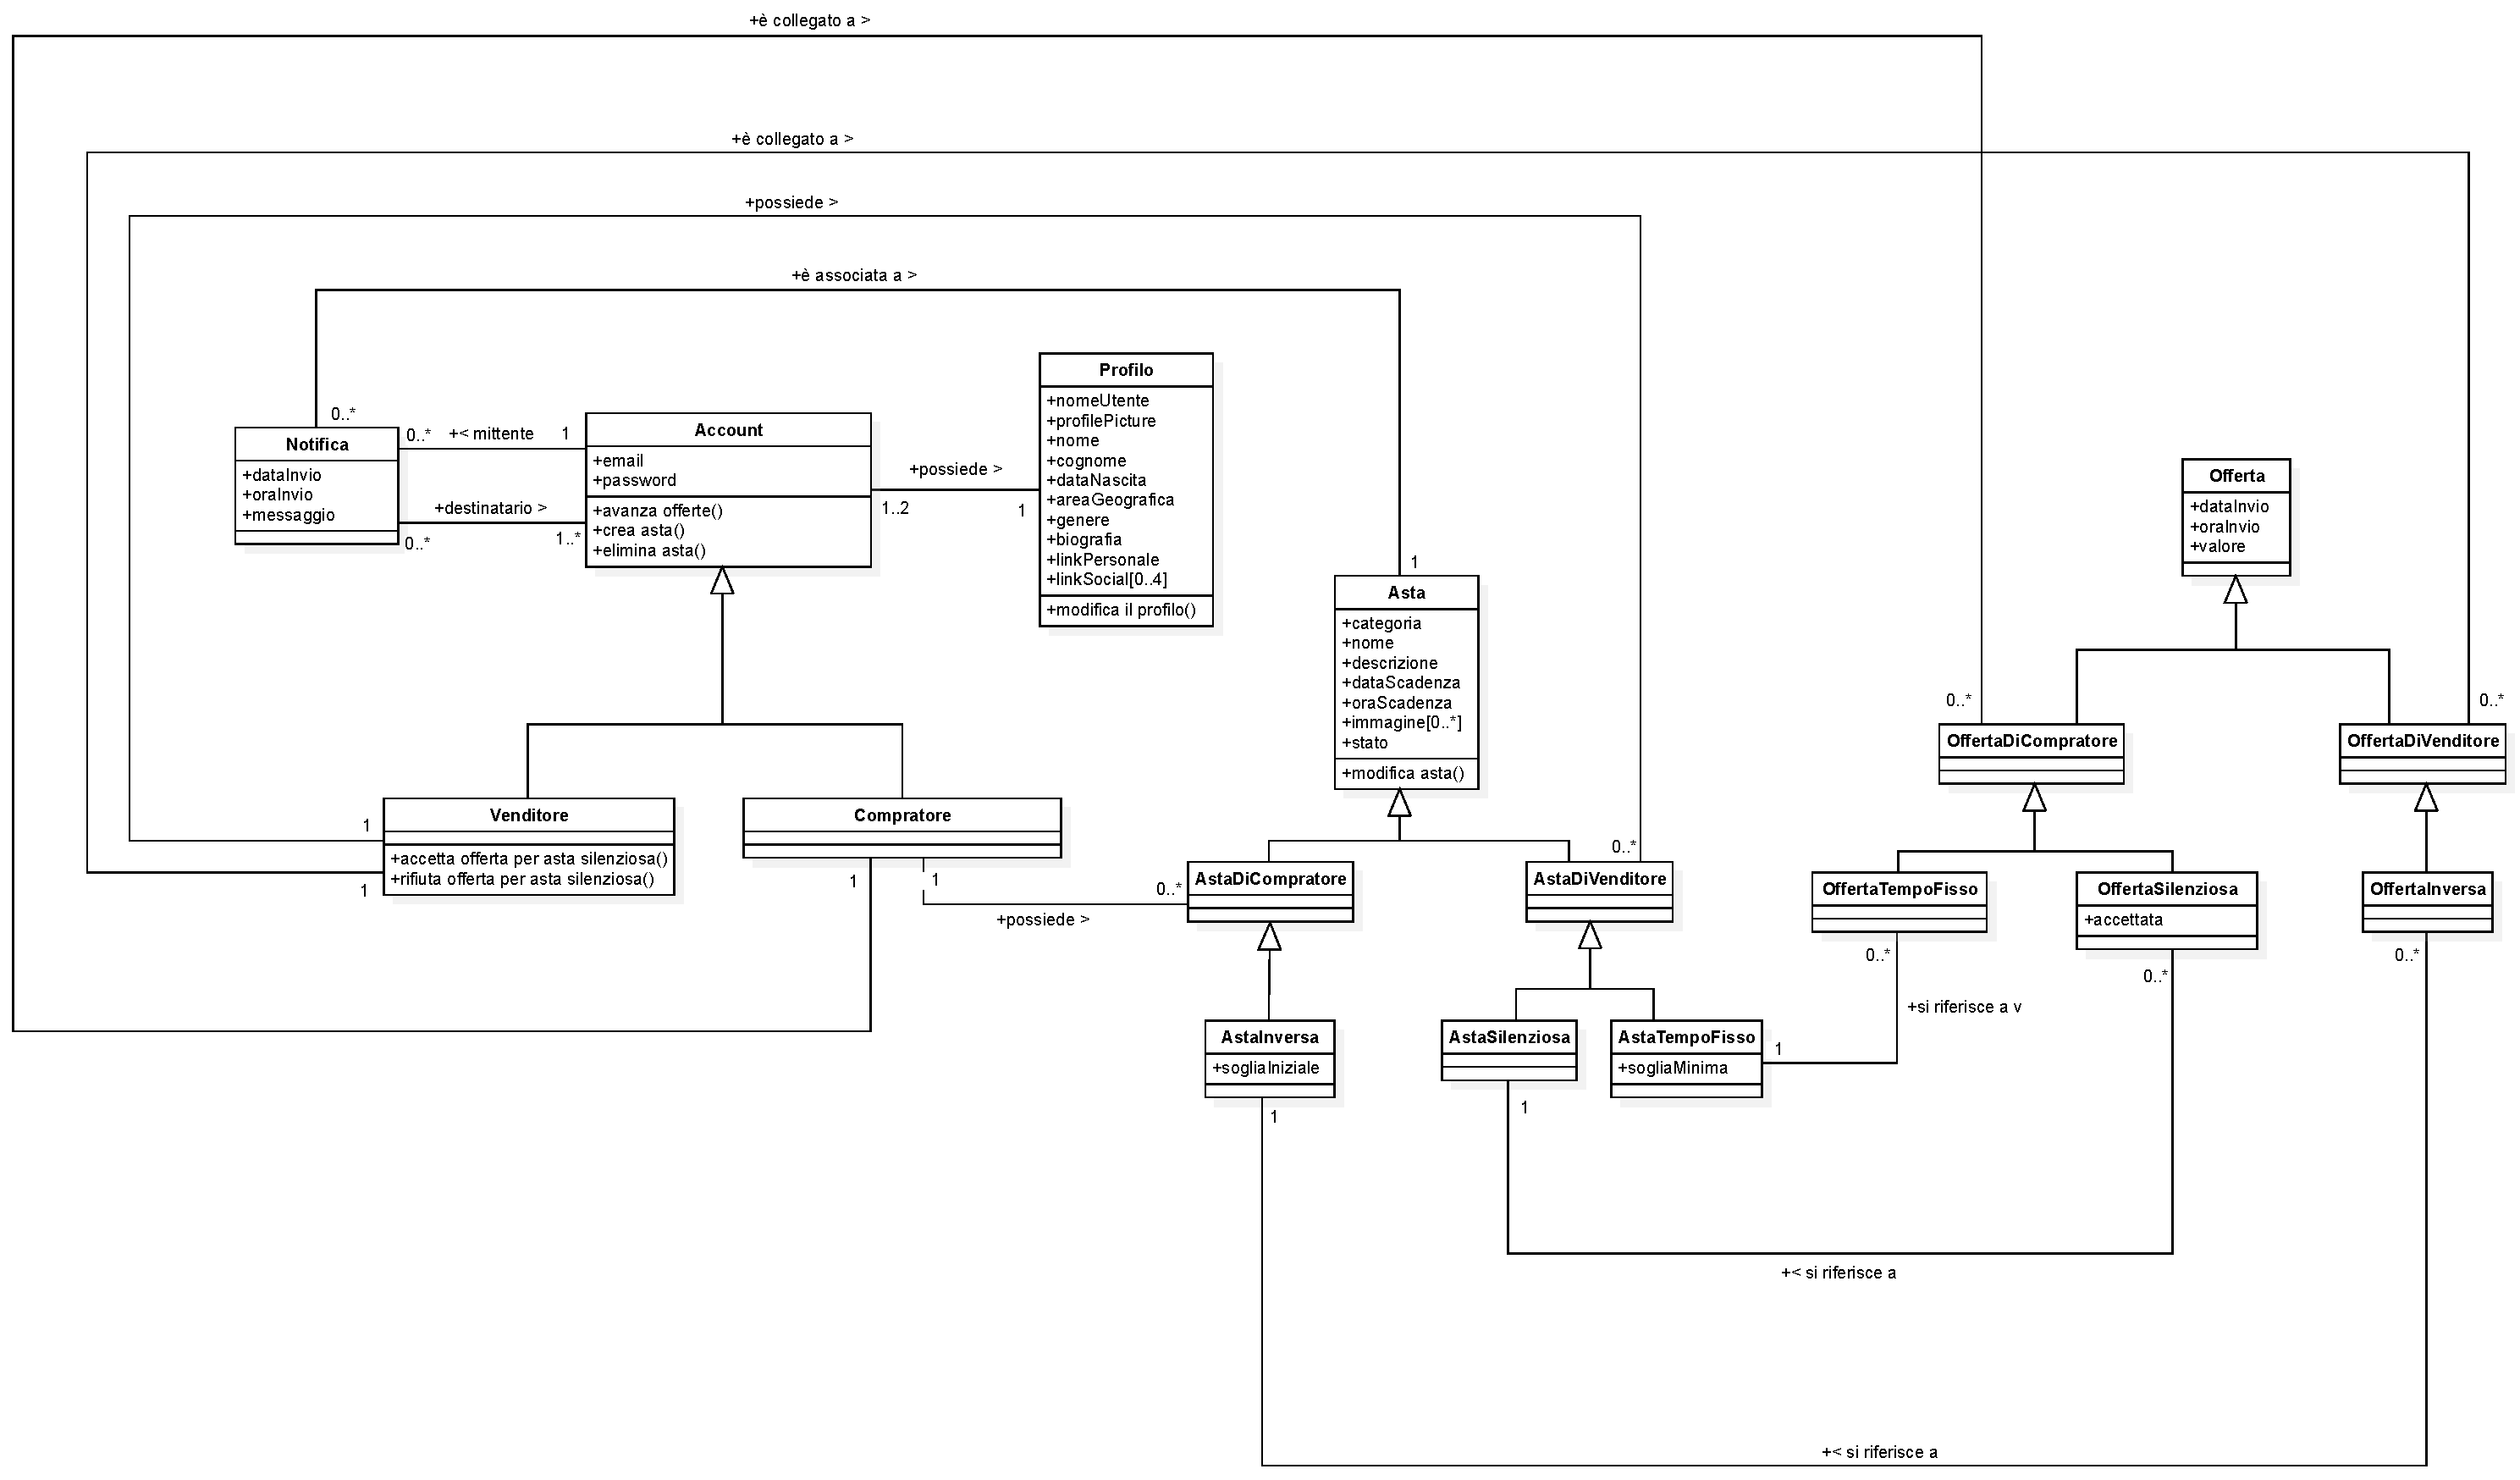
\includegraphics[width=1\linewidth]{Immagini/Diagrammi/Class Diagram/ClassDiagramDominio.pdf}
                \caption{Class Diagram del dominio del problema}
                \label{fig:Class Diagram del dominio del problema}
            \end{figure}
            
        \subsection{Class Diagram per casi d'uso}
            In questa sezione verranno mostrati i diagrammi secondo l'euristica "Three-Object-Type" per ogni caso d'uso. Le classi possono essere di tipo "boundary", "control" e "entity".
        
            \begin{figure}[htbp!]
                \centering
                    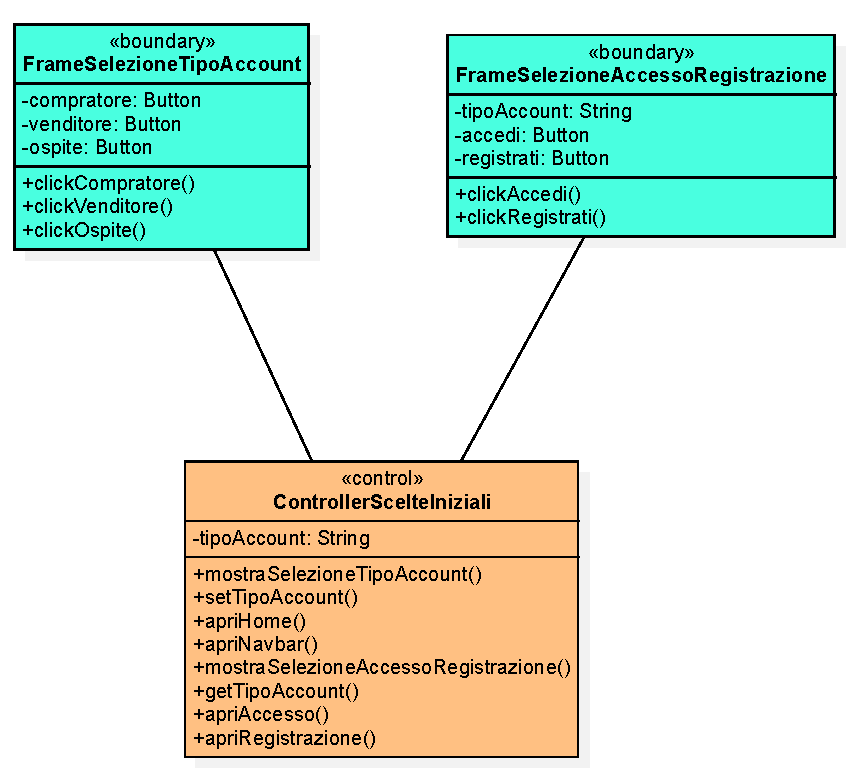
\includegraphics[width=1\linewidth]{Immagini/Diagrammi/Class Diagram/Utente che non ha effettuato l'accesso/ScelteIniziali.pdf}
                \caption{Scelta del tipo di account}
            \end{figure}
            
            \begin{figure}[htbp!]
                \centering
                    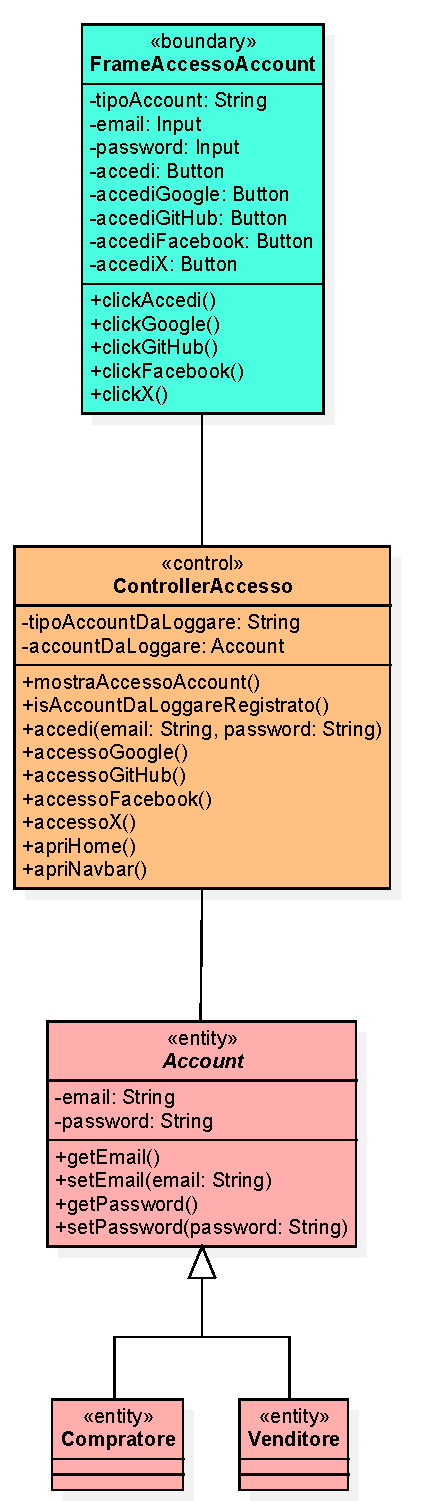
\includegraphics[width=0.35\linewidth]{Immagini/Diagrammi/Class Diagram/Utente che non ha effettuato l'accesso/Accesso.pdf}
                \caption{Accesso}
            \end{figure}
            
            \begin{figure}[htbp!]
                \centering
                    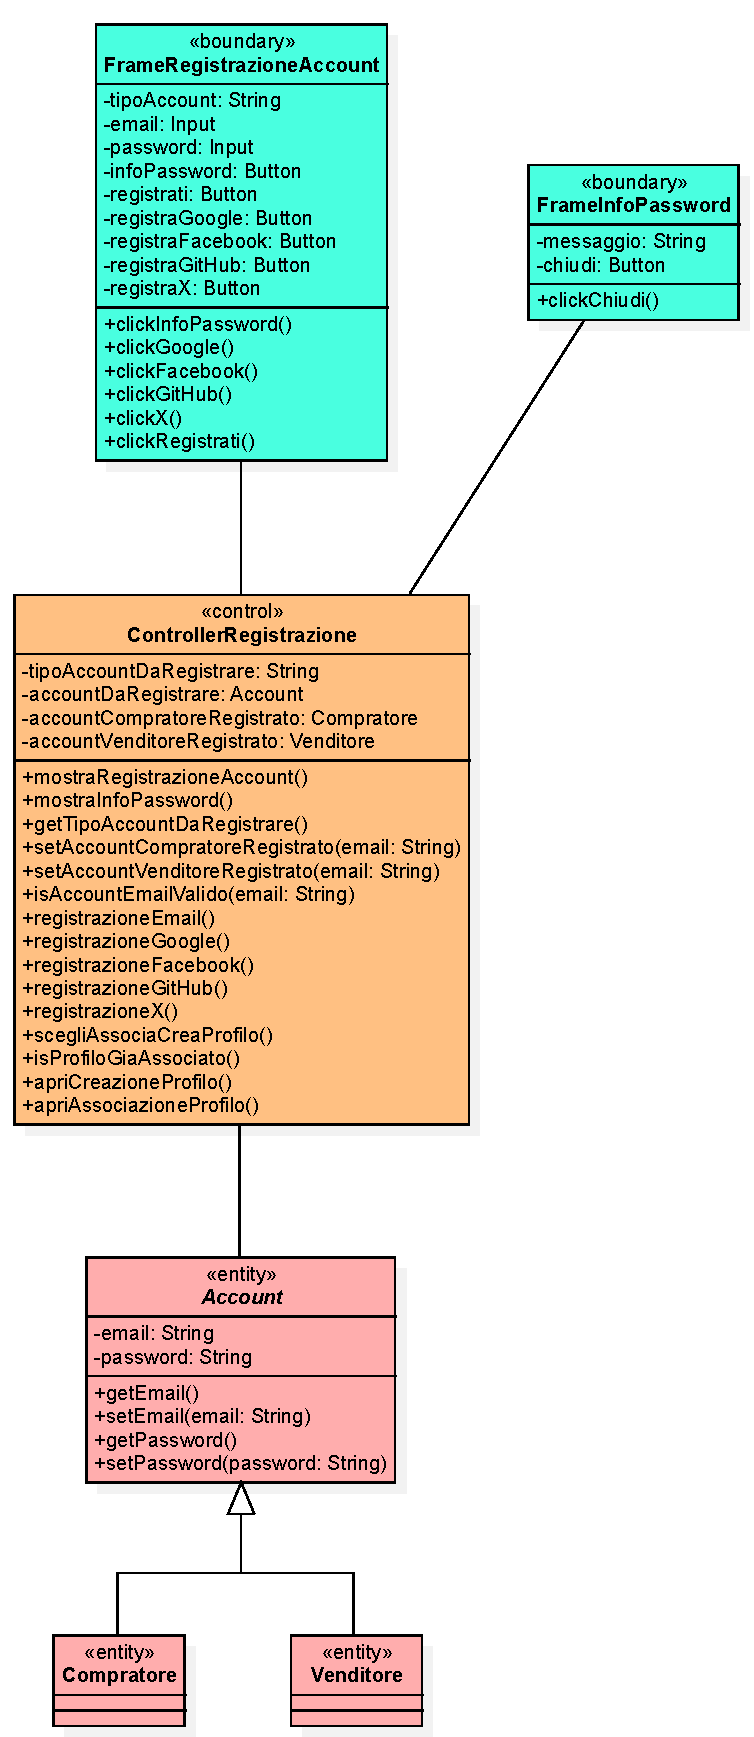
\includegraphics[width=0.55\linewidth]{Immagini/Diagrammi/Class Diagram/Utente che non ha effettuato l'accesso/Registrazione.pdf}
                \caption{Registrazione}
            \end{figure}
            
            \begin{figure}[htbp!]
                \centering
                    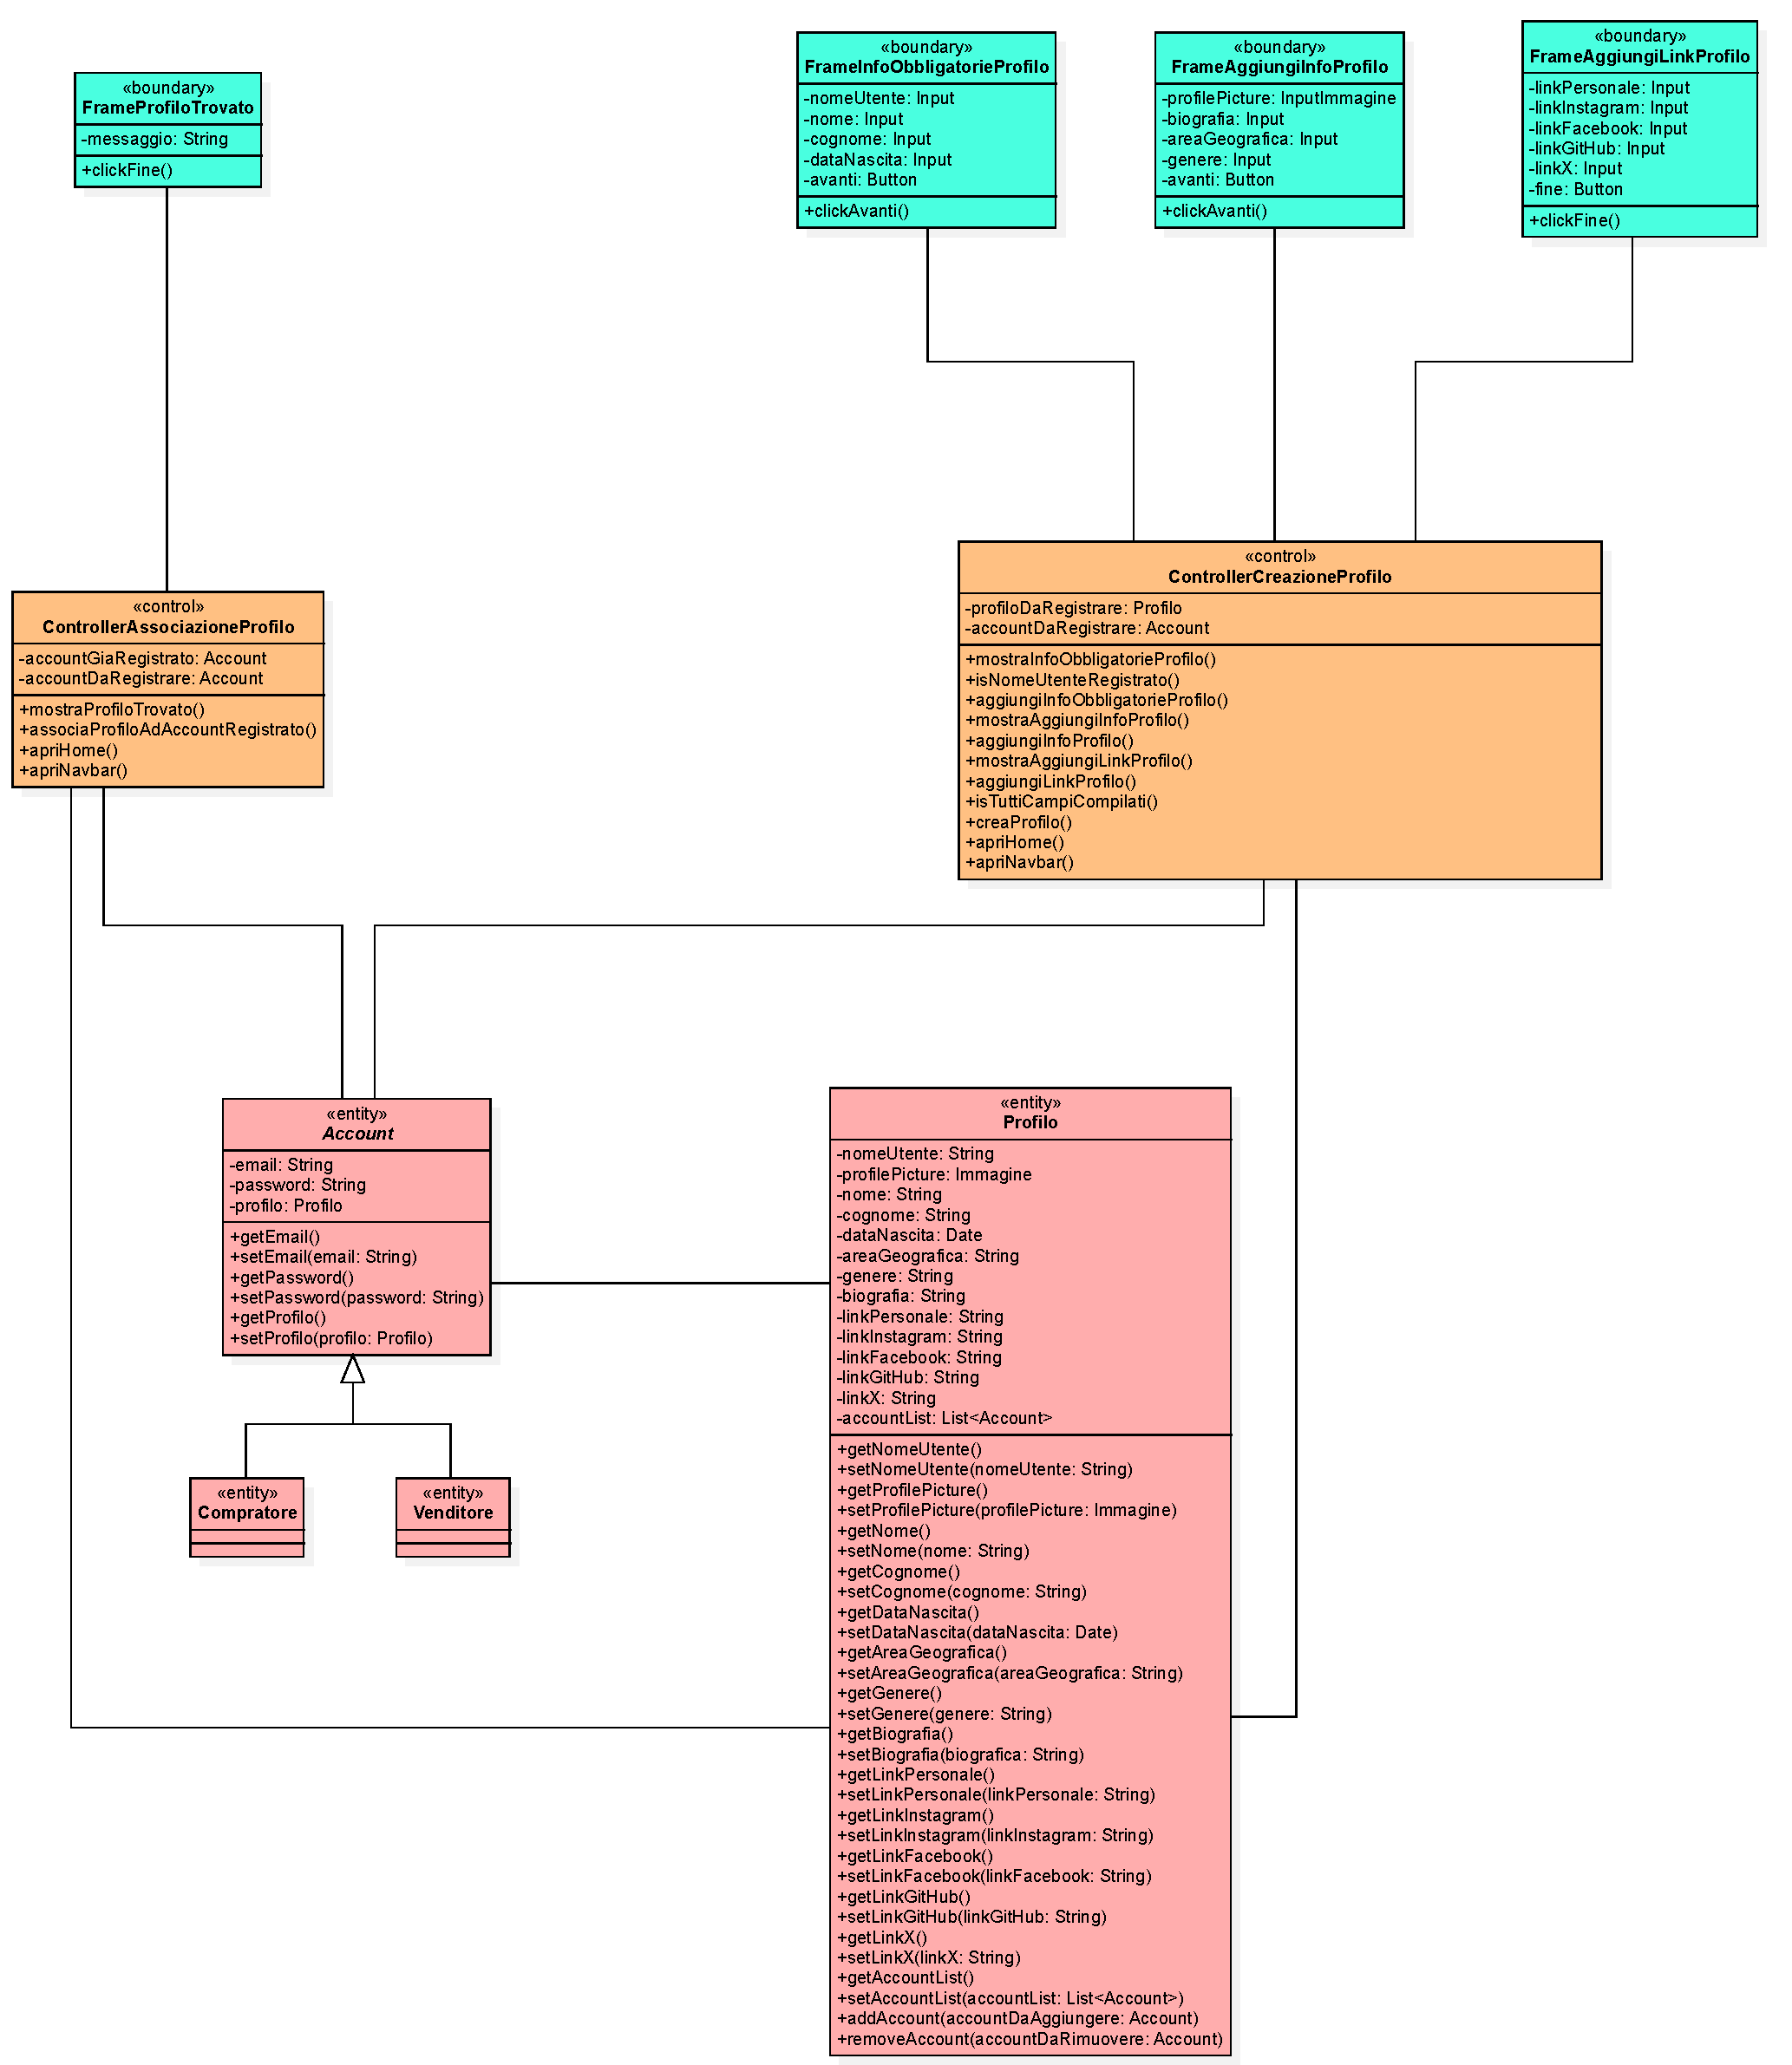
\includegraphics[width=1\linewidth]{Immagini/Diagrammi/Class Diagram/Utente che non ha effettuato l'accesso/CreazioneProfilo.pdf}
                \caption{Creazione del profilo}
            \end{figure}
            
            \begin{figure}[htbp!]
                \centering
                    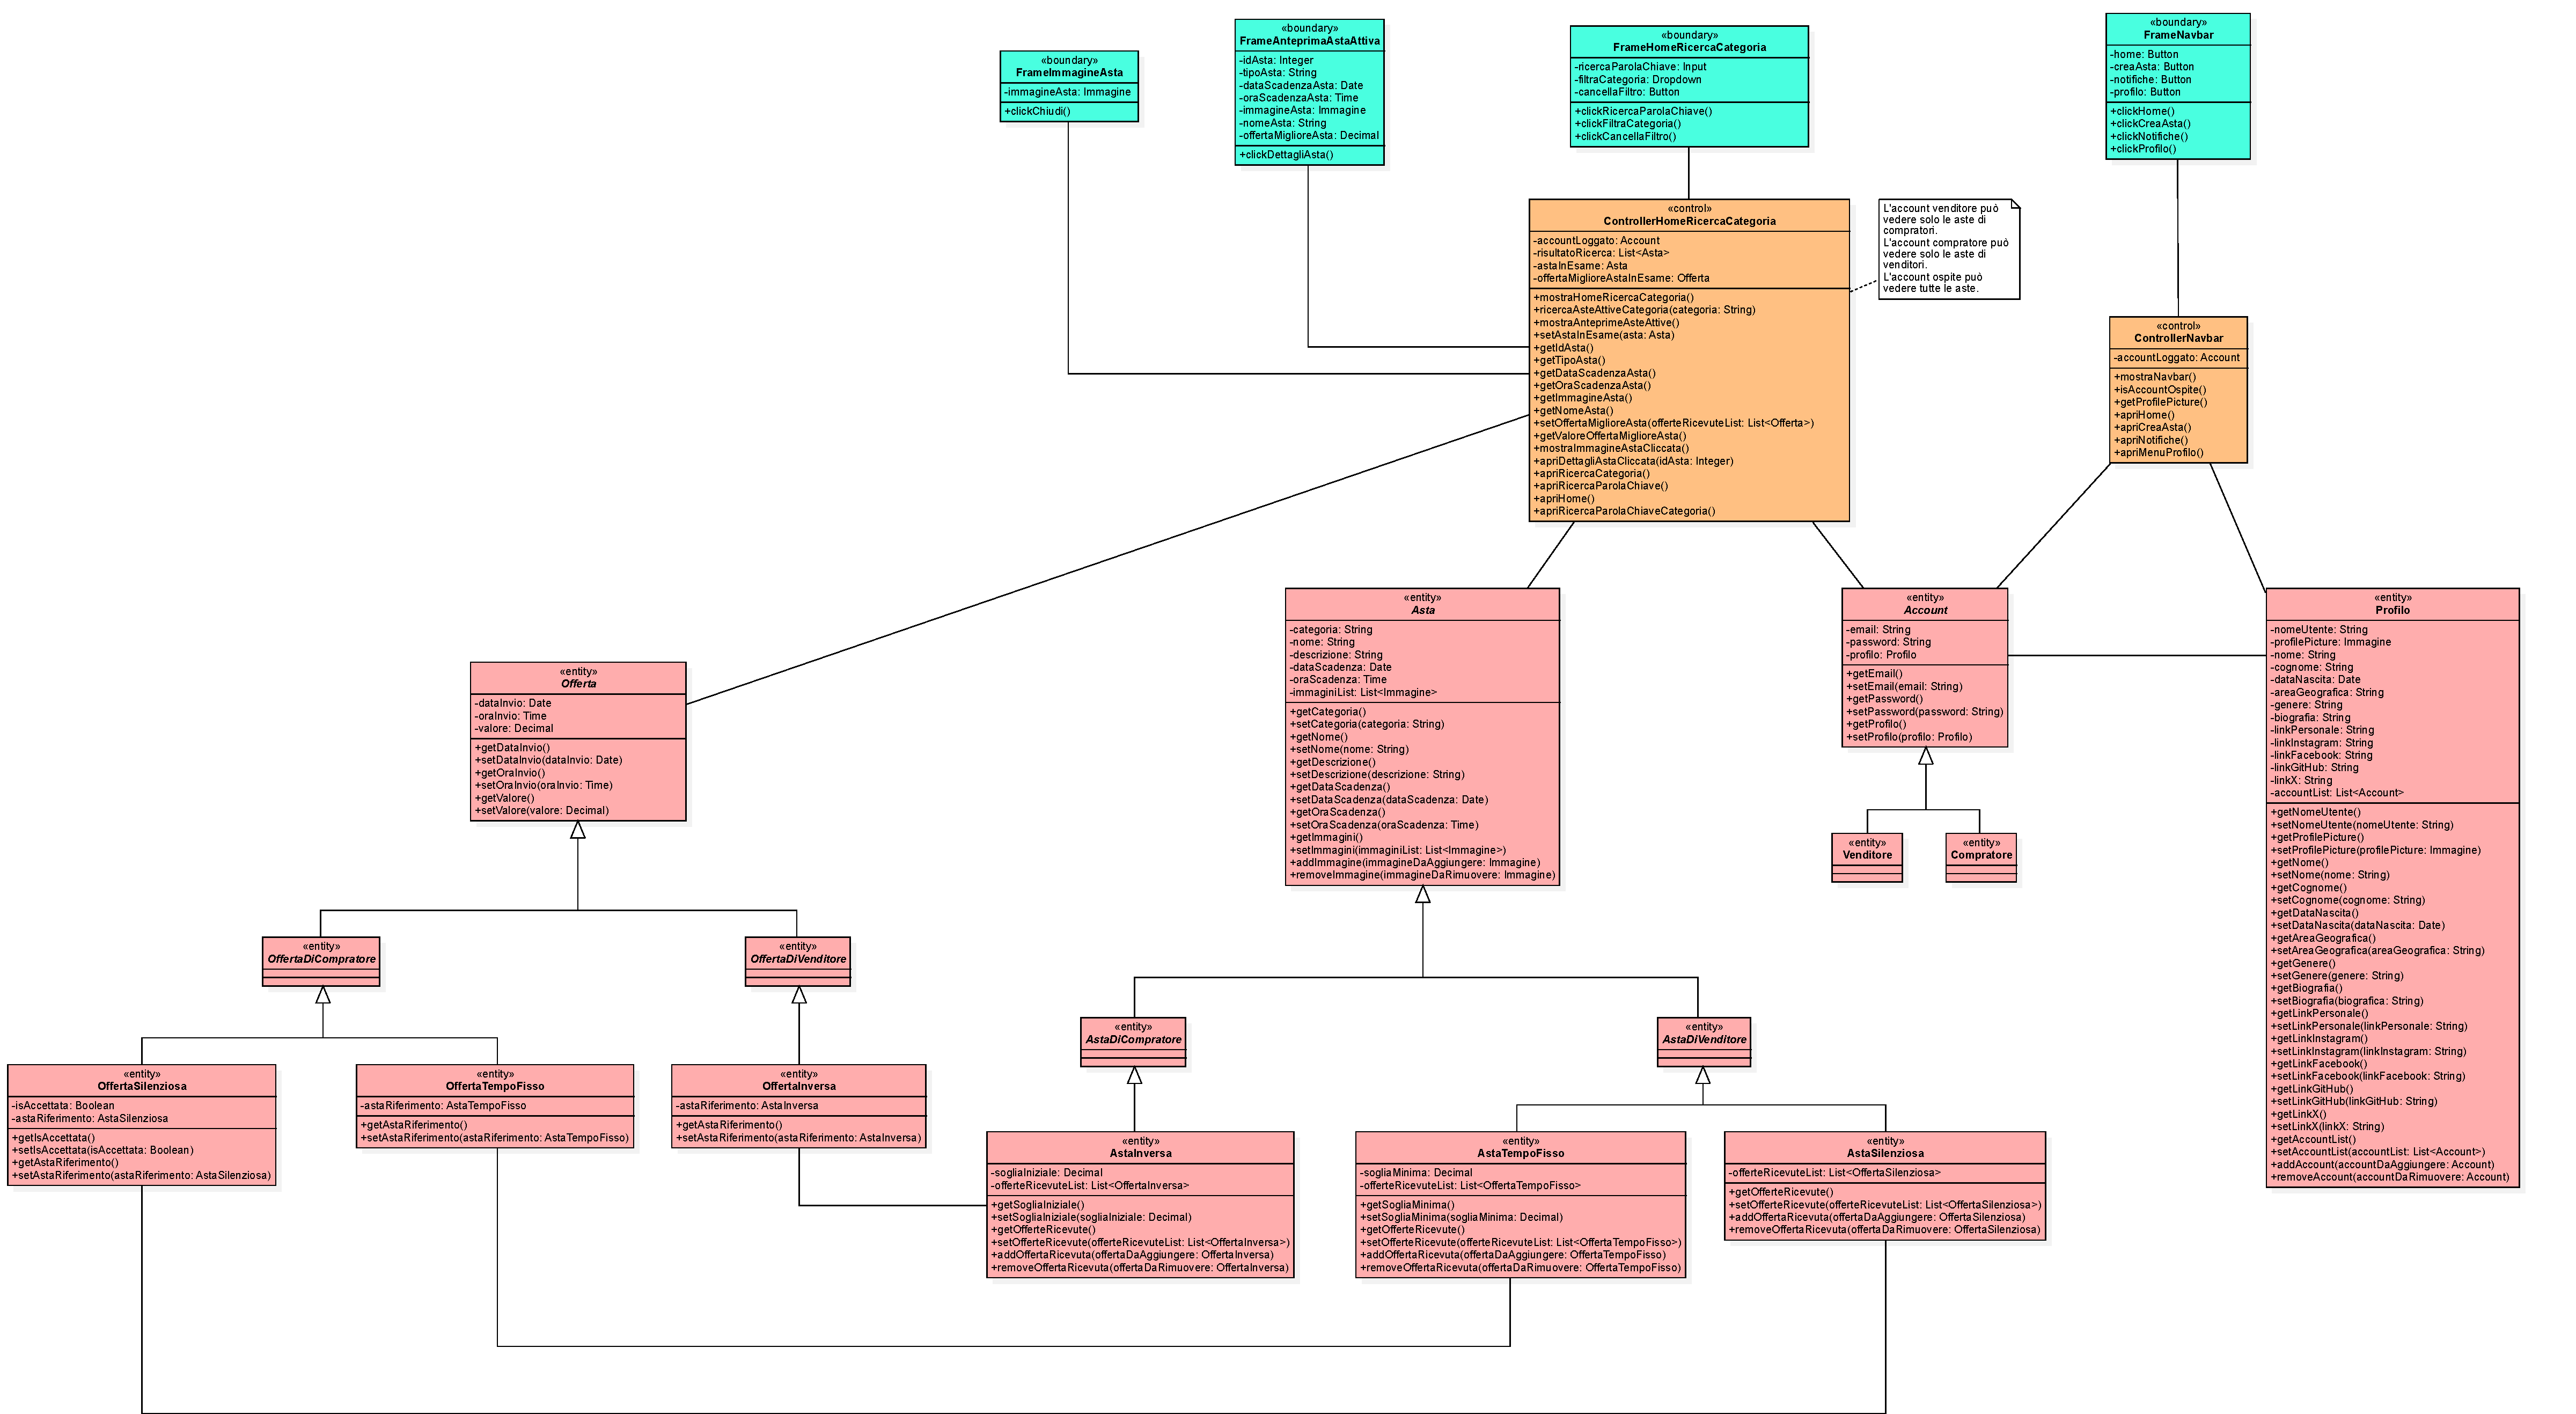
\includegraphics[width=1\linewidth]{Immagini/Diagrammi/Class Diagram/Utente generico/RicercaCategoria.pdf}
                \caption{Ricerca per categoria}
            \end{figure}
            
            \begin{figure}[htbp!]
                \centering
                    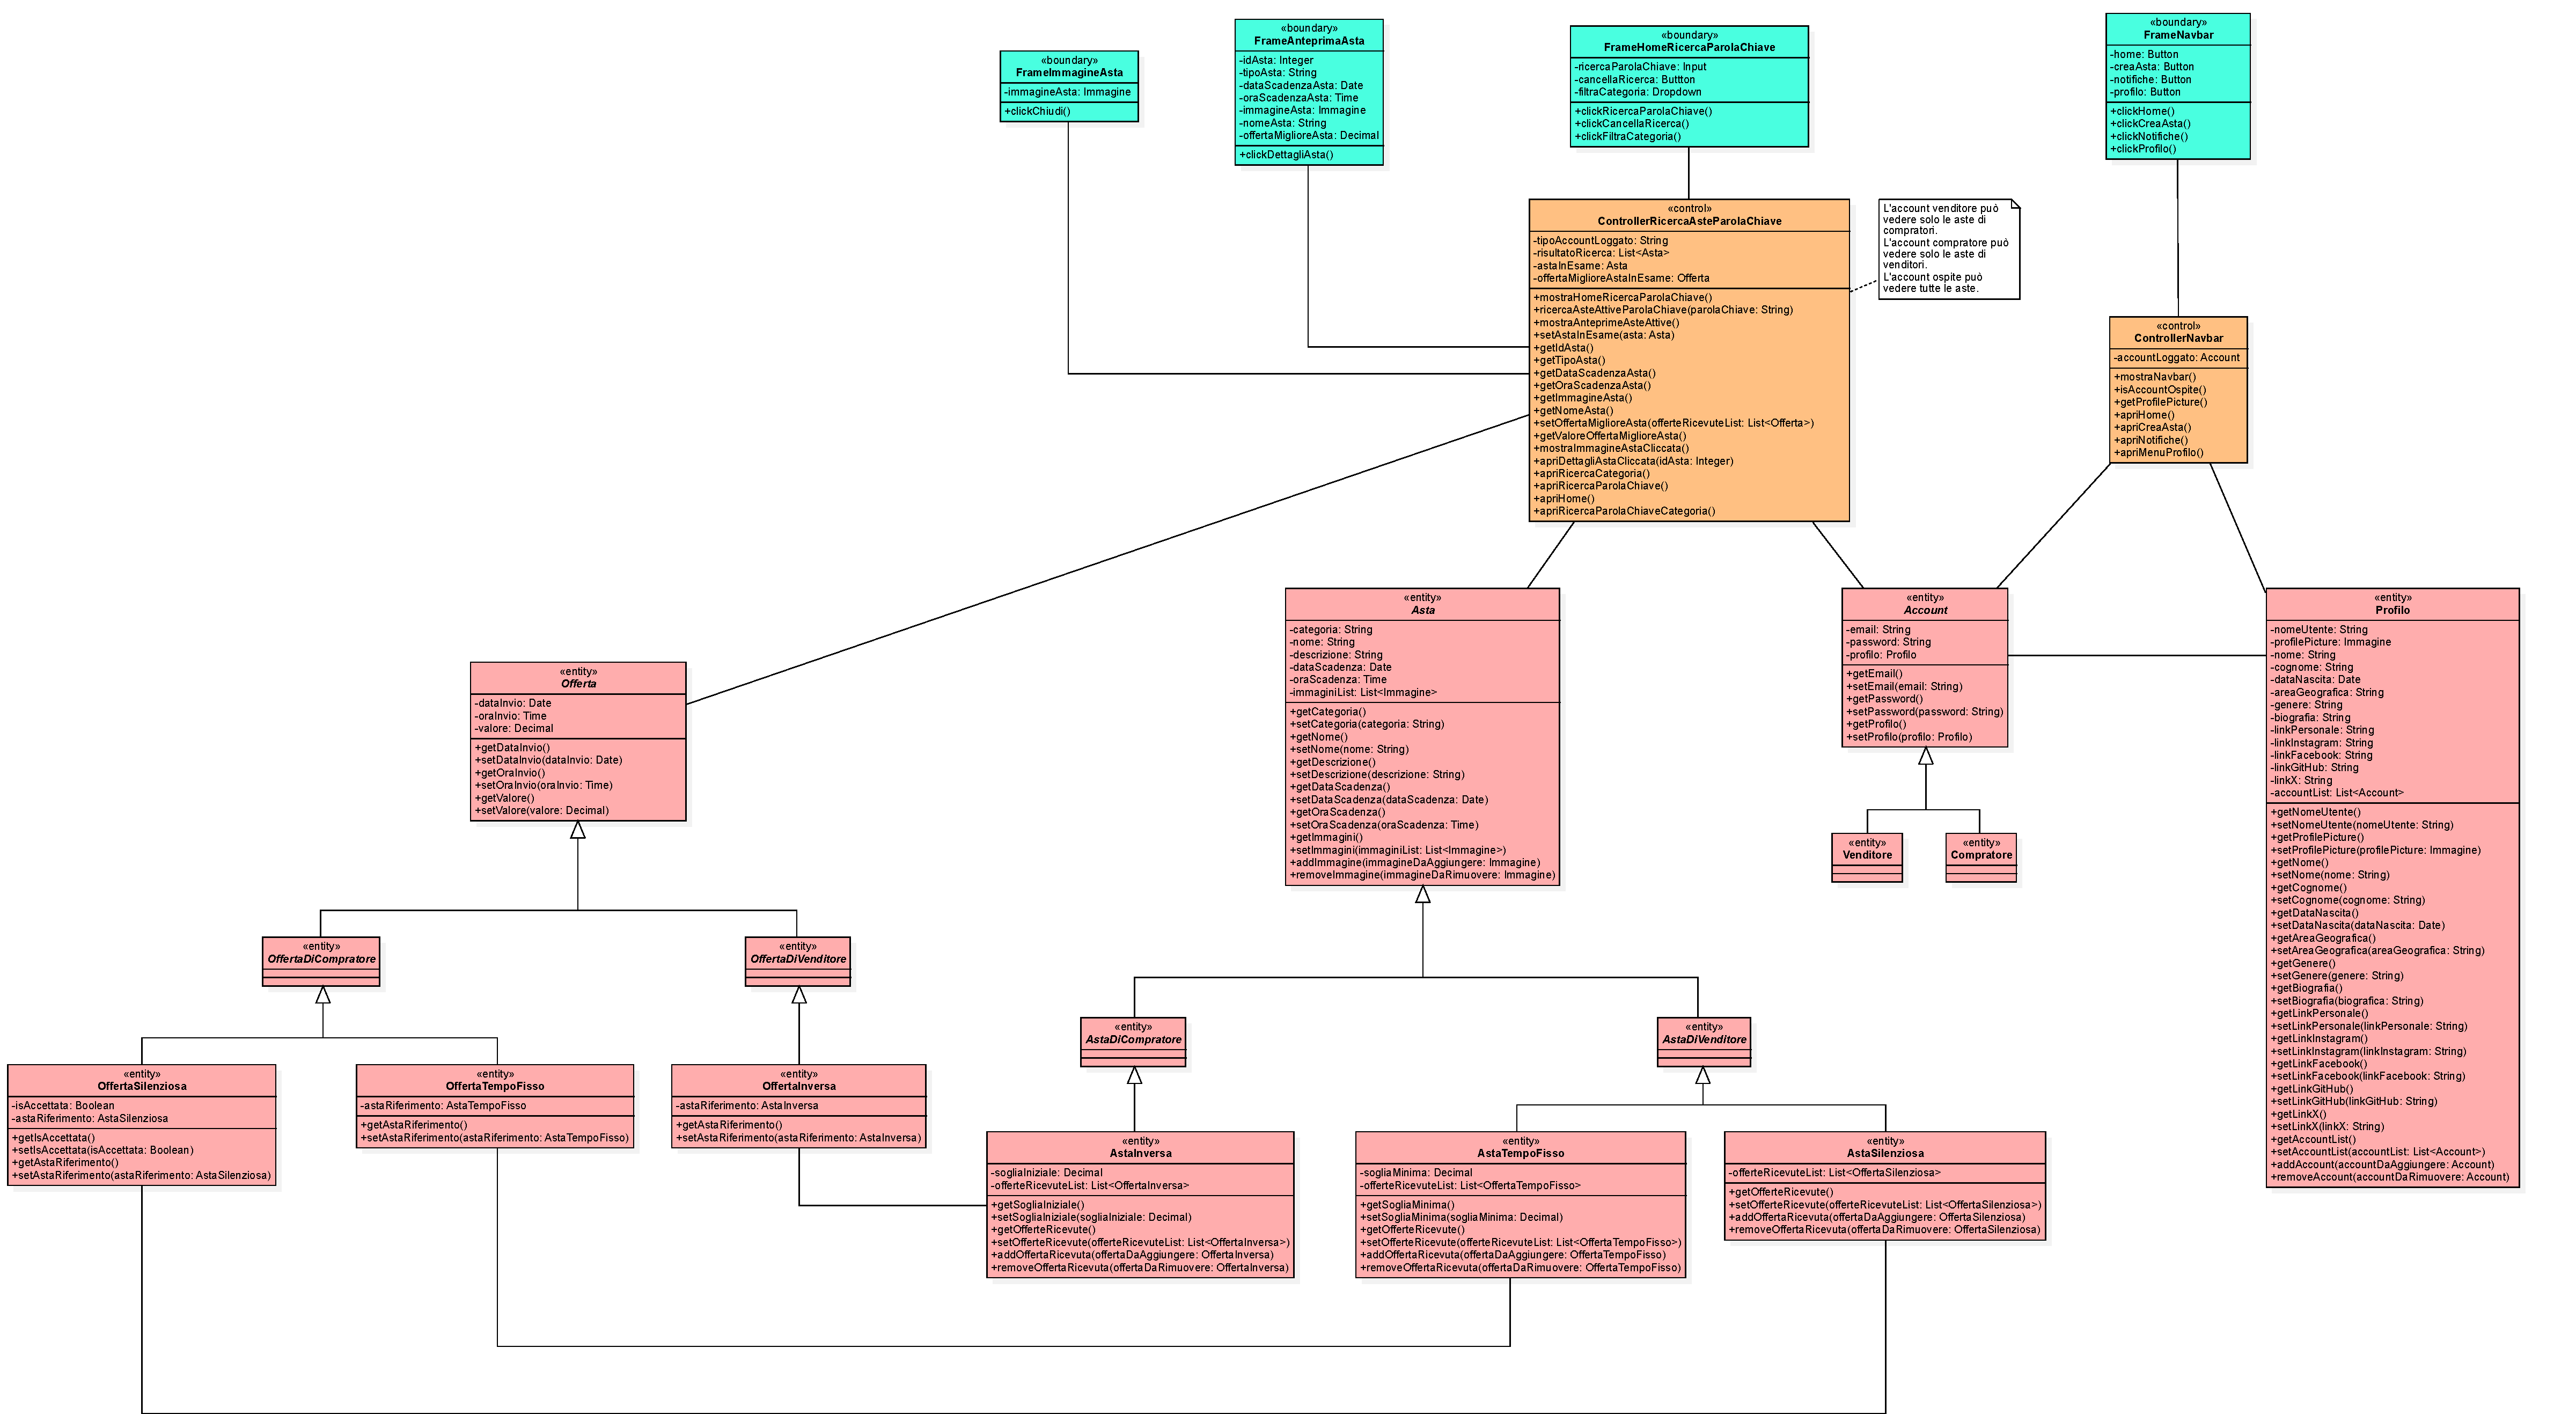
\includegraphics[width=1\linewidth]{Immagini/Diagrammi/Class Diagram/Utente generico/RicercaParolaChiave.pdf}
                \caption{Ricerca per parola chiave}
            \end{figure}
            
            \begin{figure}[htbp!]
                \centering
                    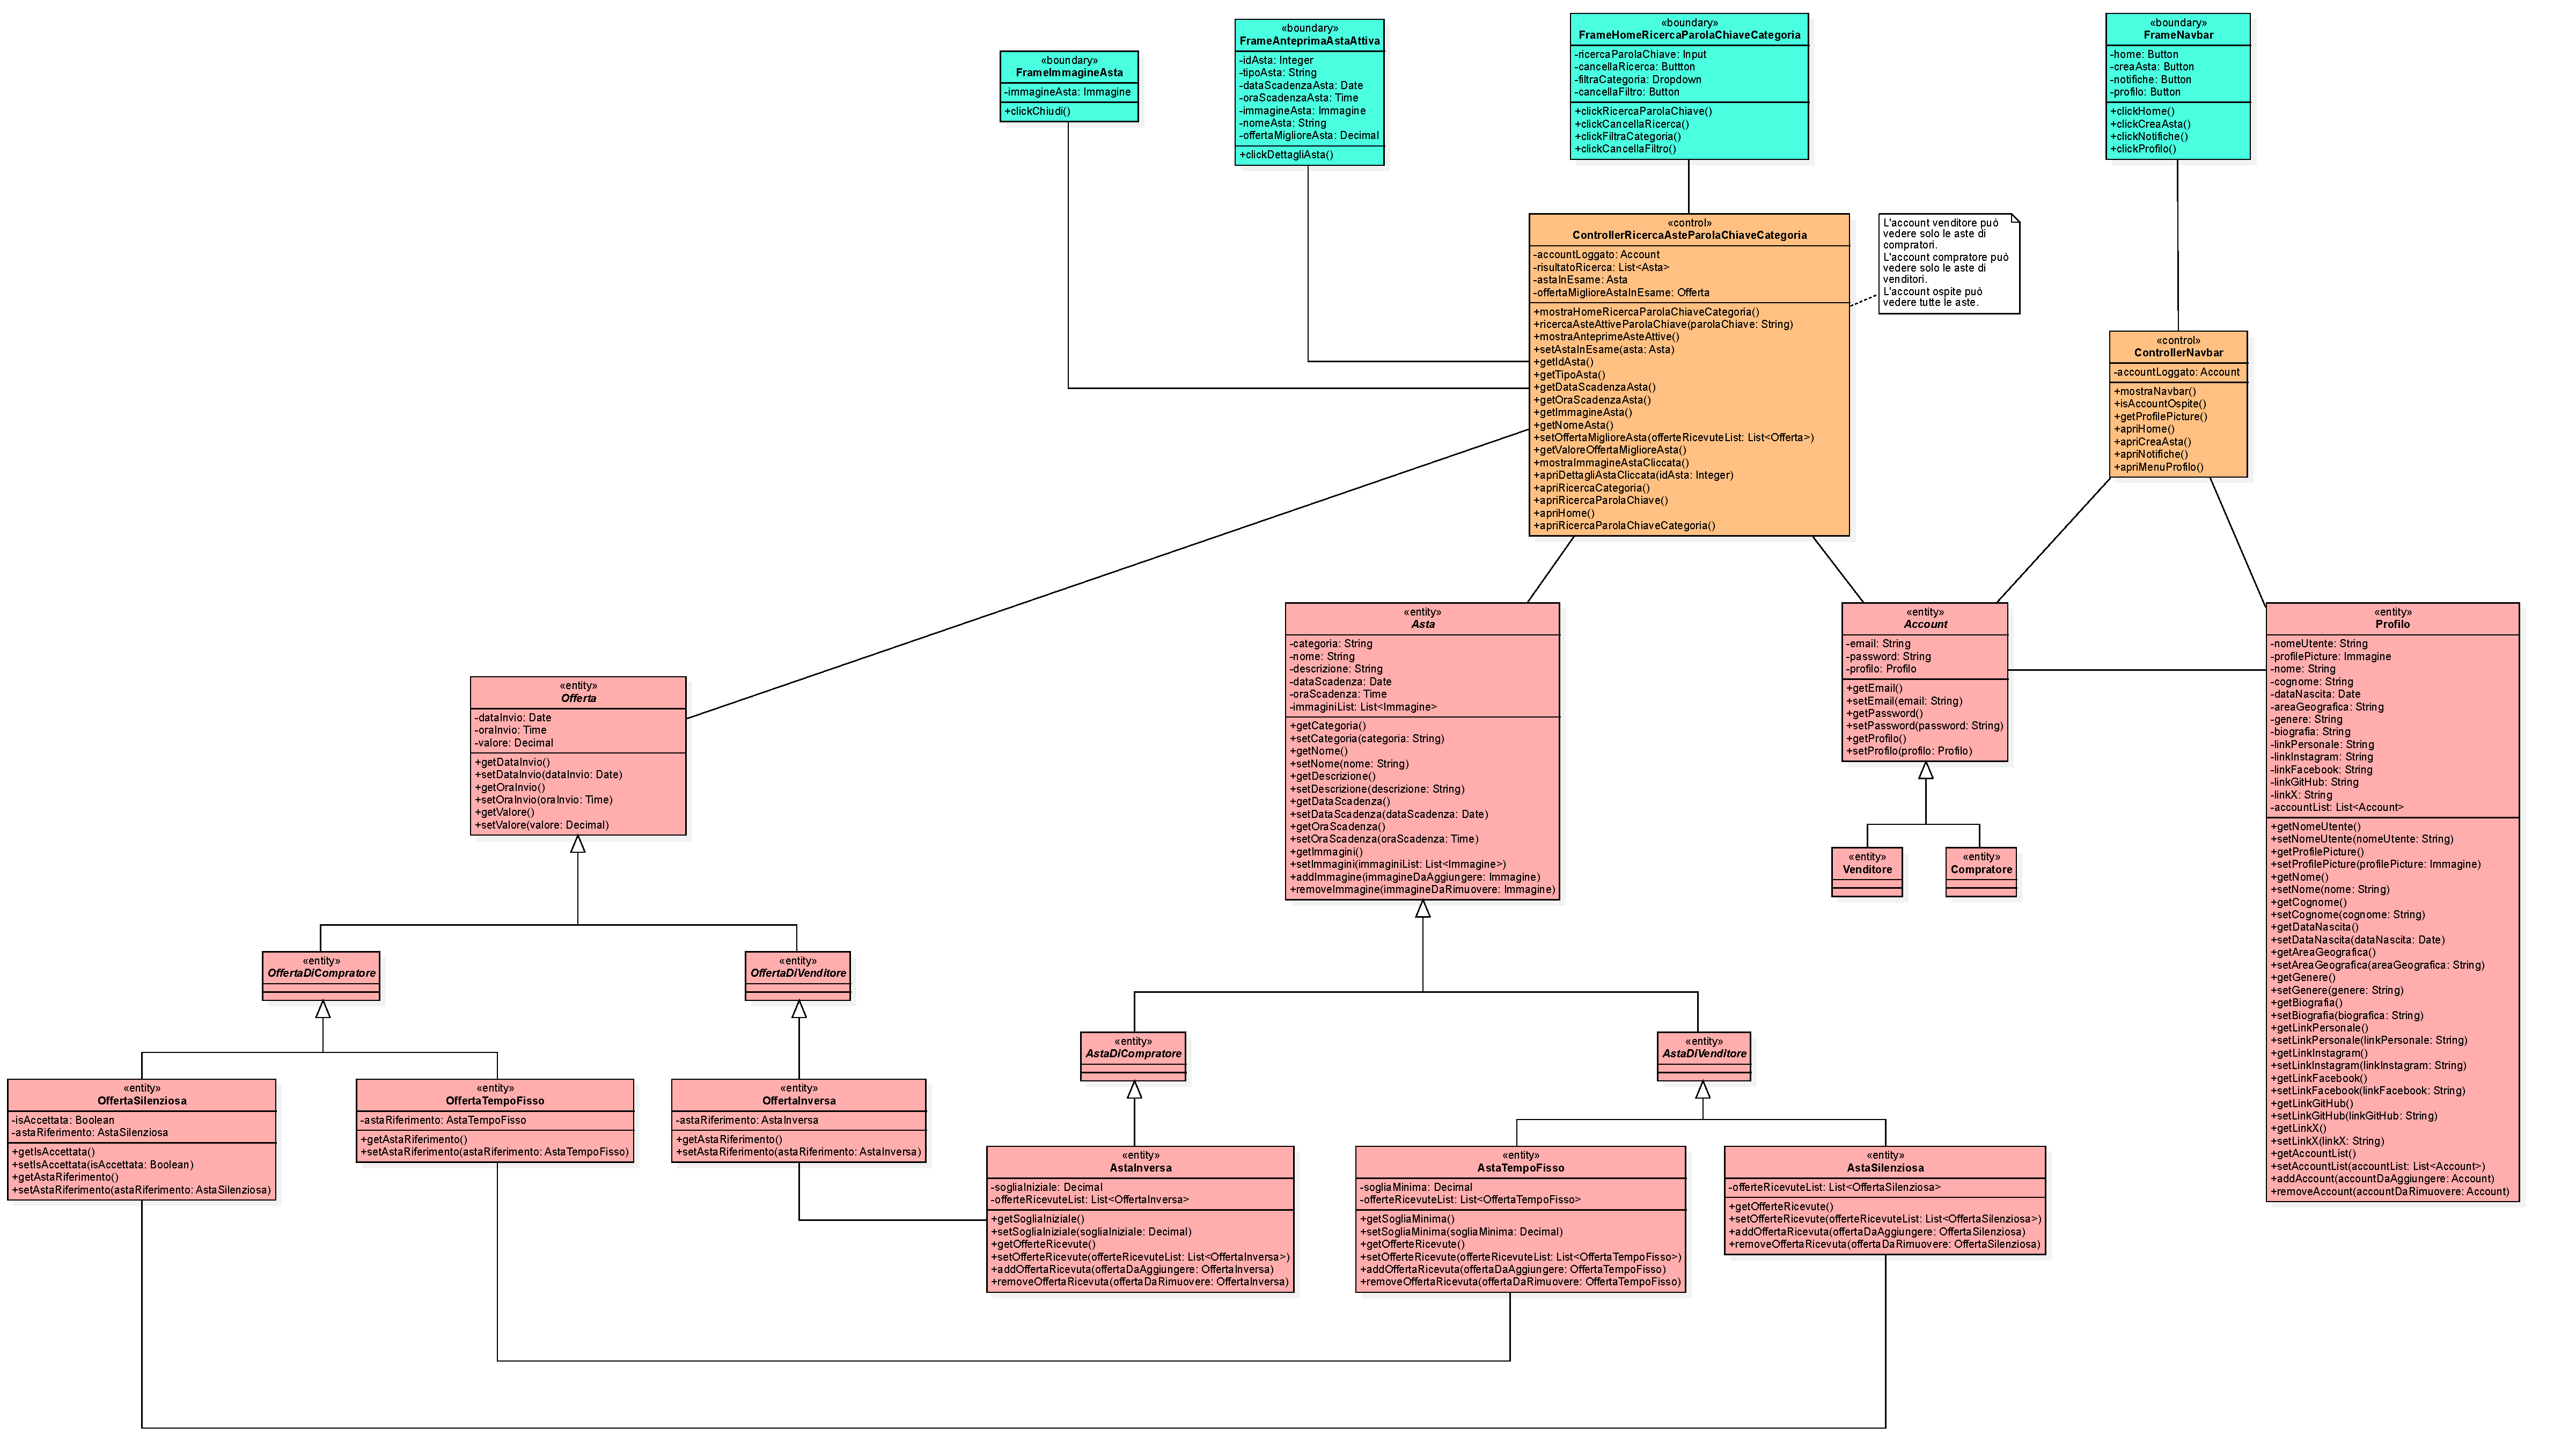
\includegraphics[width=1\linewidth]{Immagini/Diagrammi/Class Diagram/Utente generico/RicercaParolaChiaveCategoria.pdf}
                \caption{Ricerca per parola chiave e categoria}
            \end{figure}
            
            \begin{figure}[htbp!]
                \centering
                    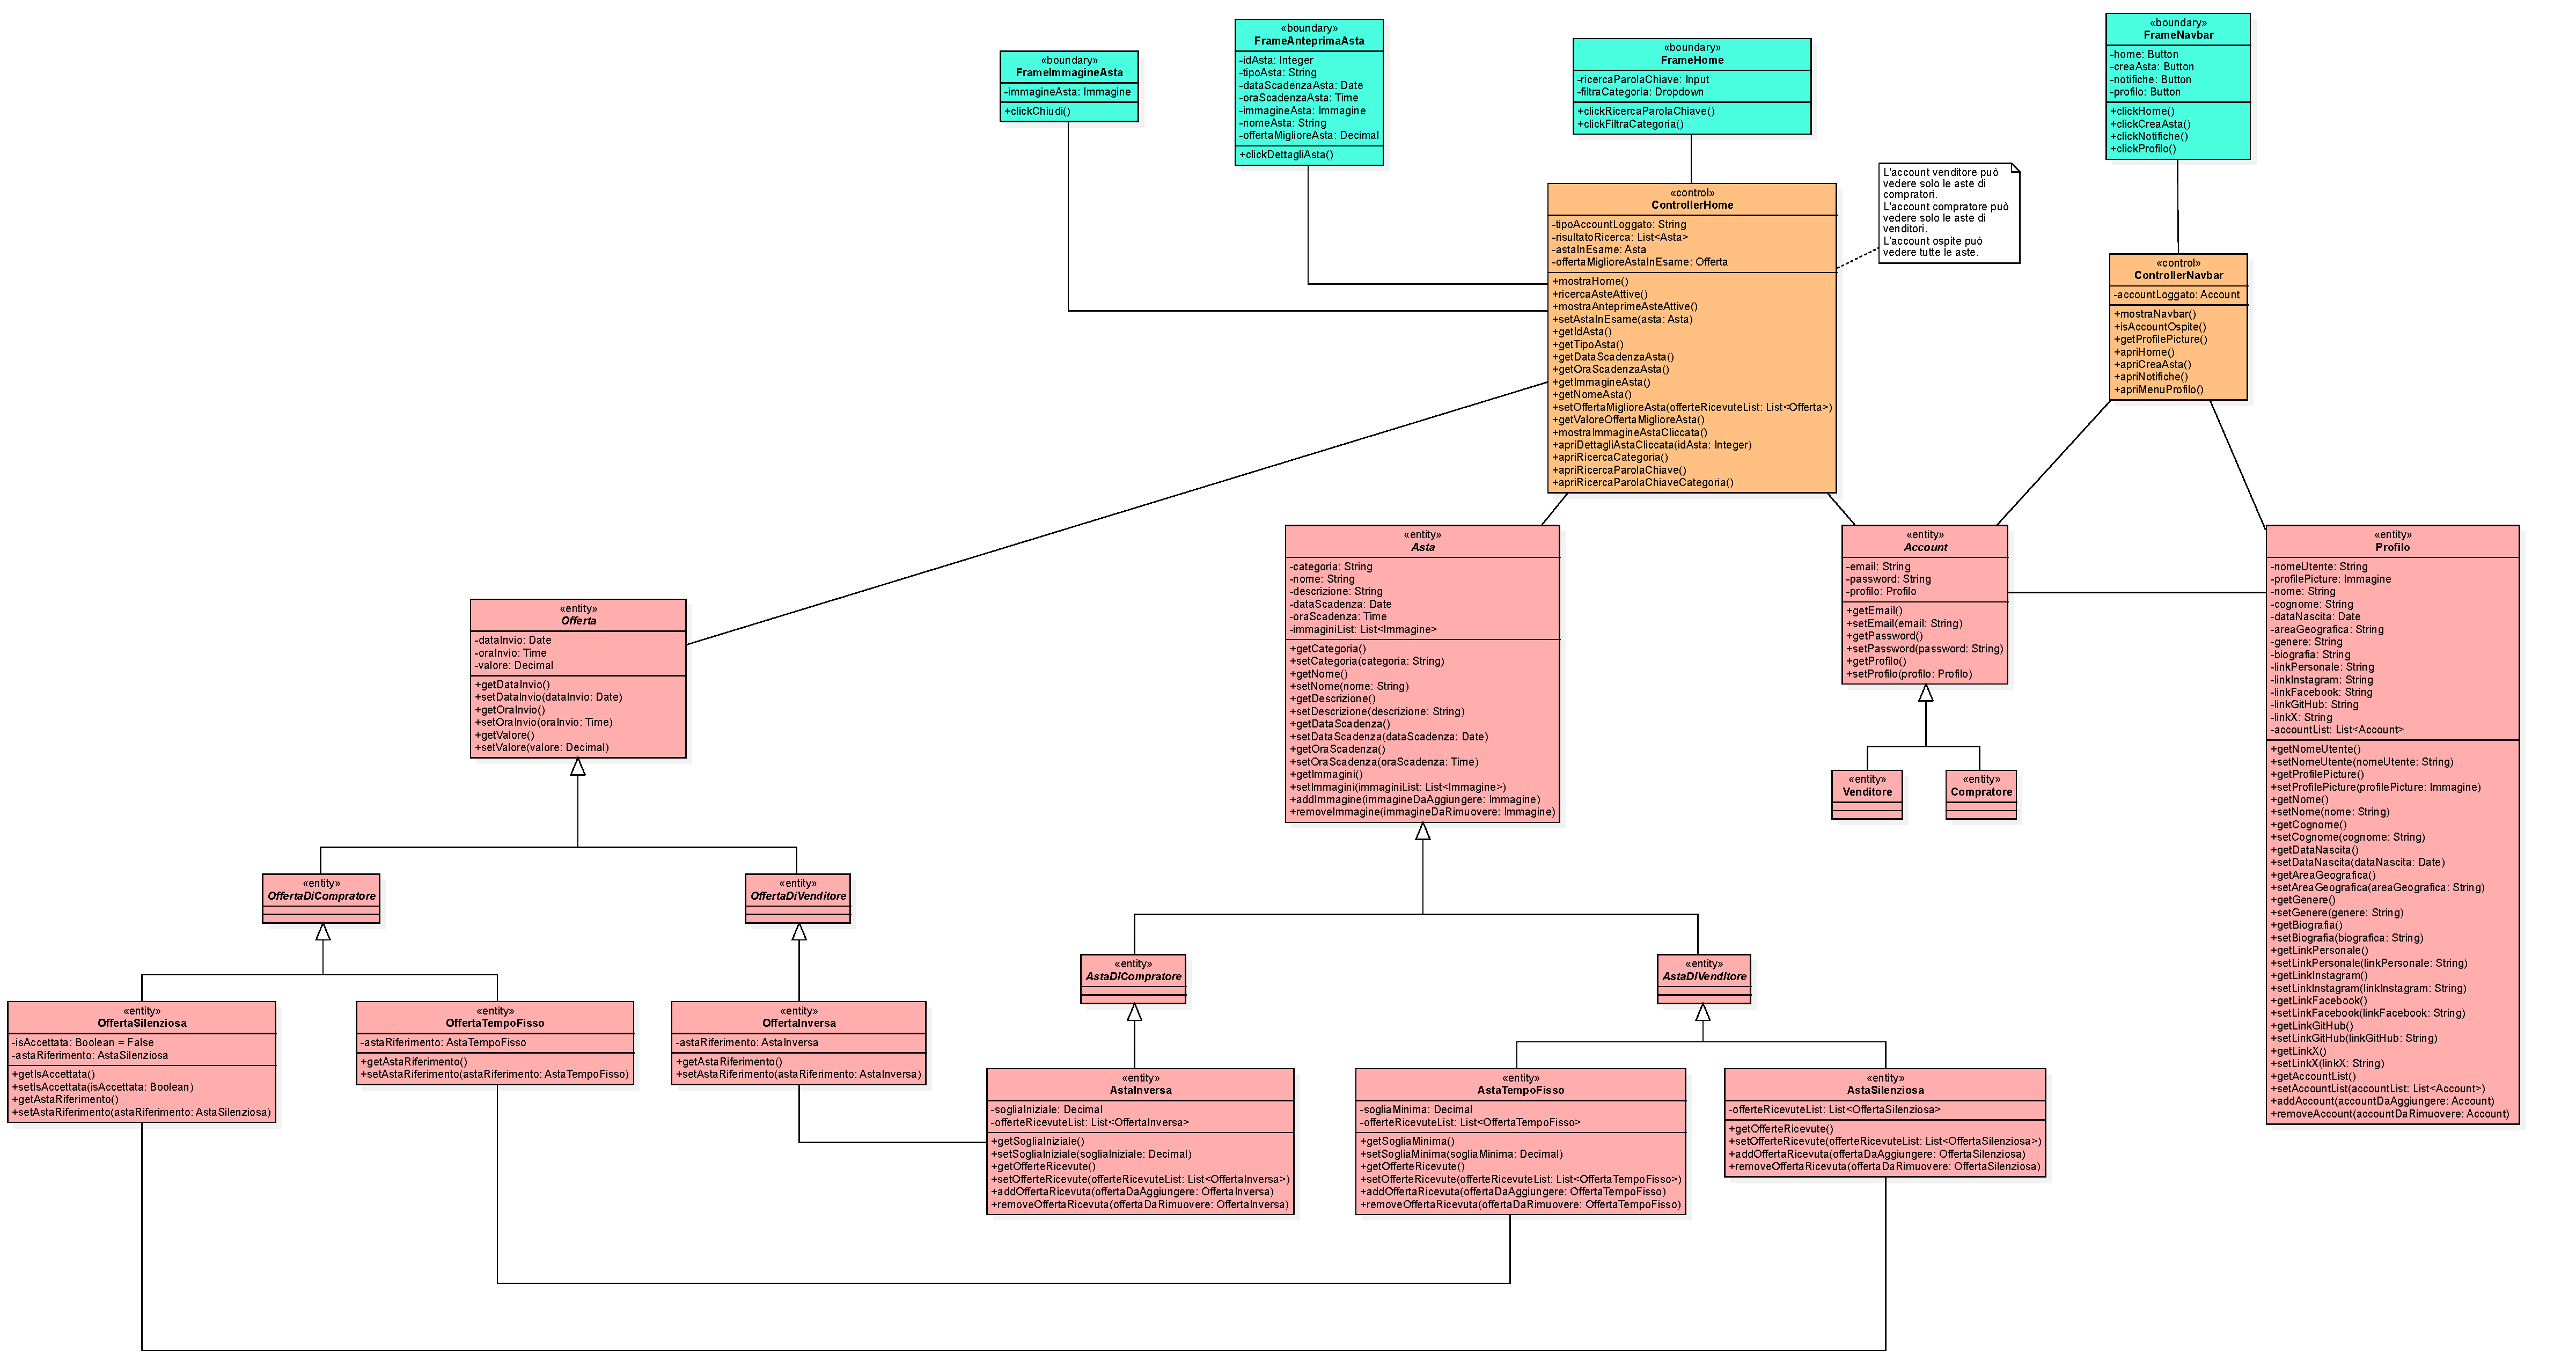
\includegraphics[width=1\linewidth]{Immagini/Diagrammi/Class Diagram/Utente generico/VisualizzaAsteAttive.pdf}
                \caption{Visualizza aste attive}
            \end{figure}
            
            \begin{figure}[htbp!]
                \centering
                    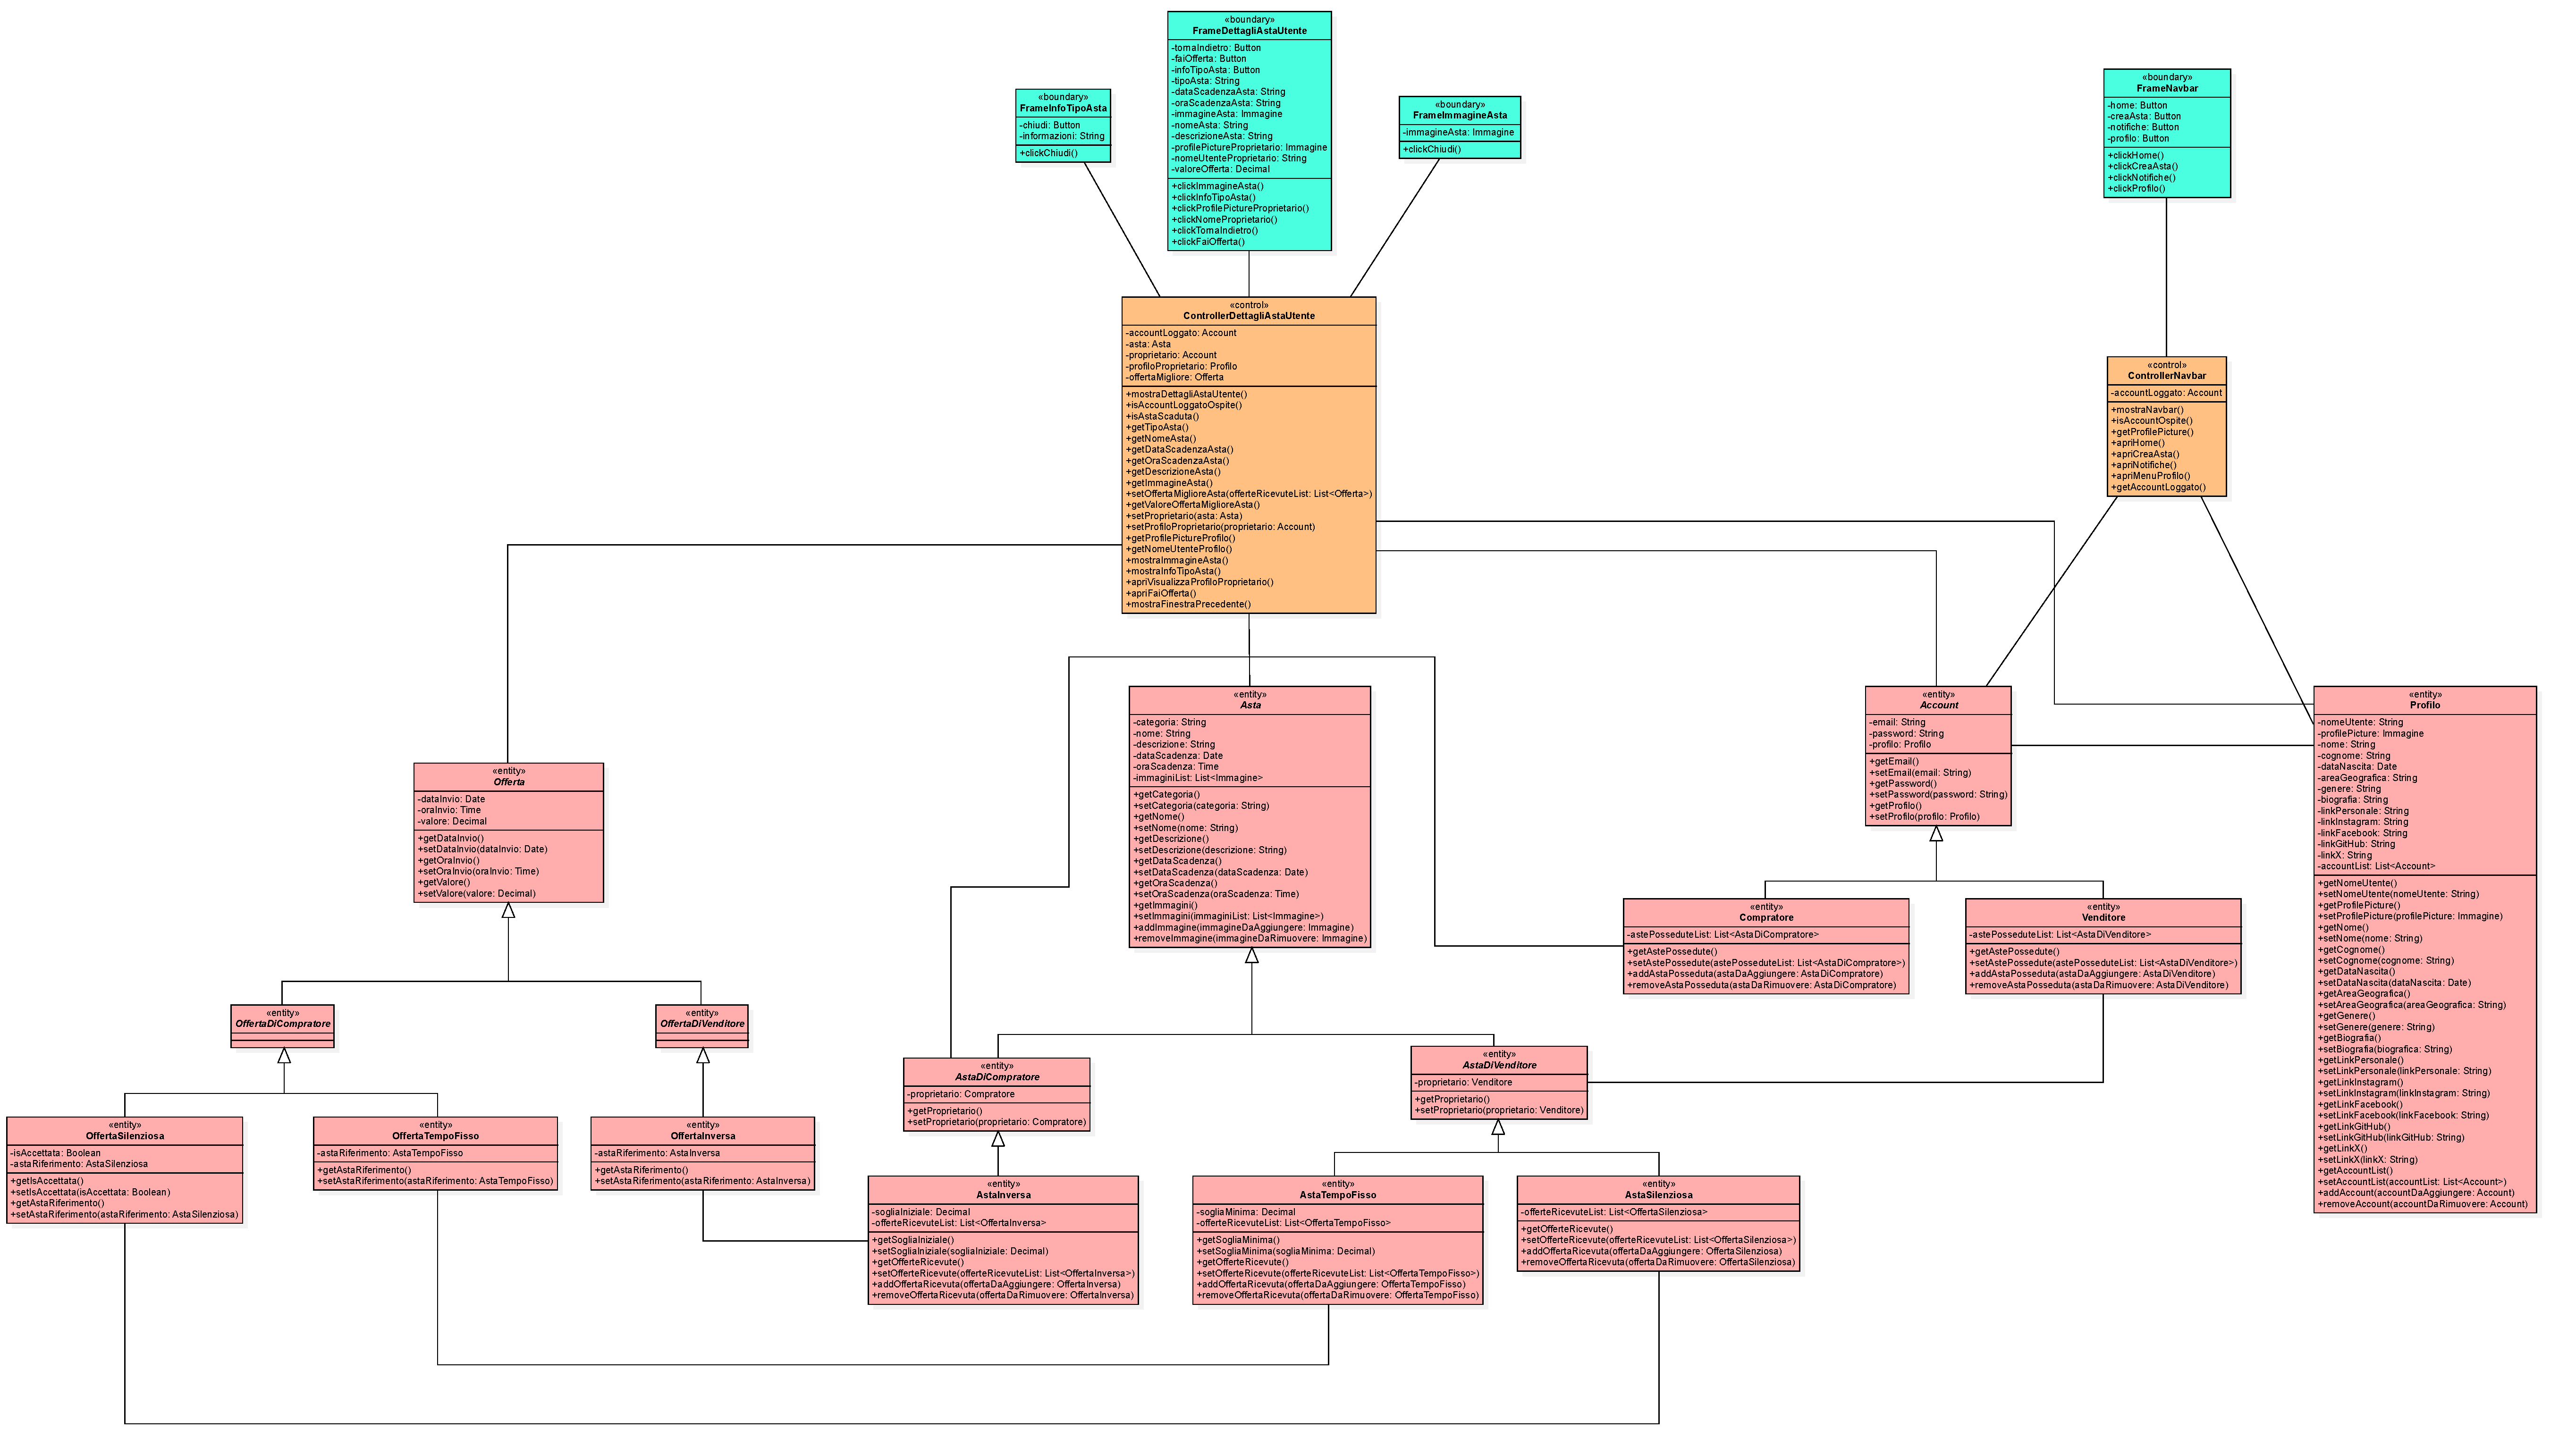
\includegraphics[width=1\linewidth]{Immagini/Diagrammi/Class Diagram/Utente generico/VisualizzaDettagliAstaUtente.pdf}
                \caption{Visualizza dettagli asta di un altro utente}
            \end{figure}
            
            \begin{figure}[htbp!]
                \centering
                    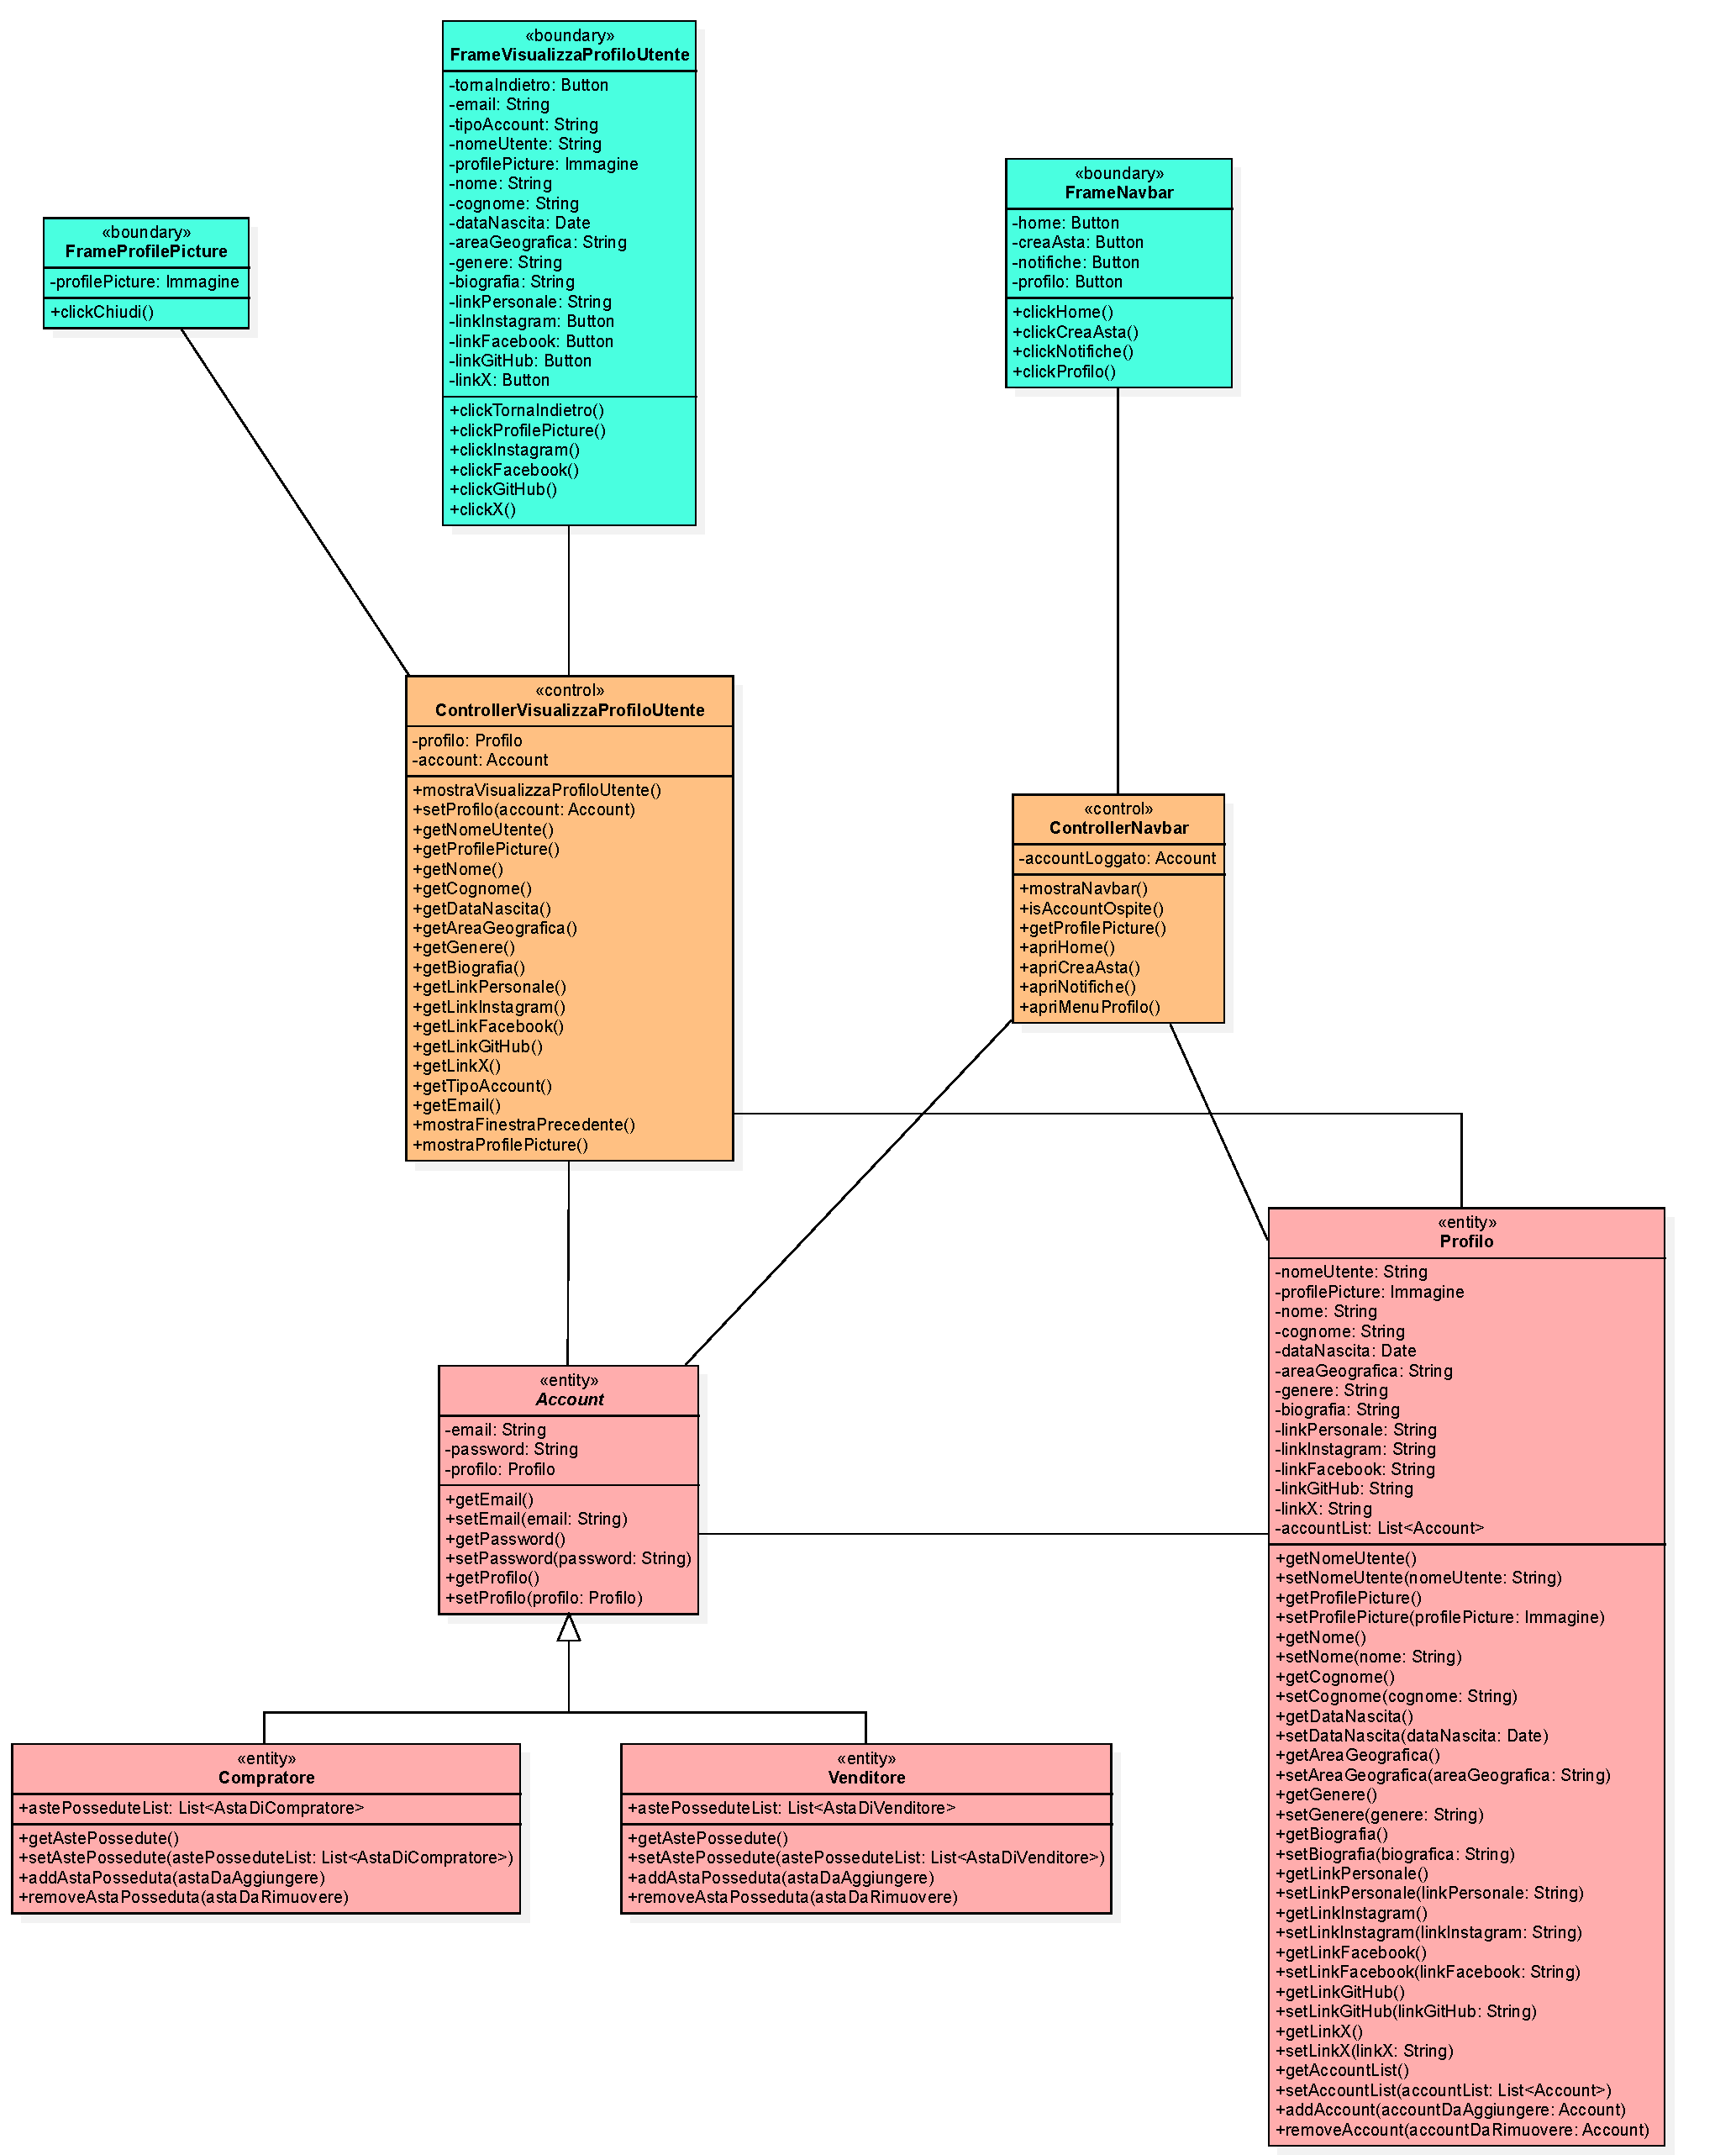
\includegraphics[width=1\linewidth]{Immagini/Diagrammi/Class Diagram/Utente generico/VisualizzaProfiloUtente.pdf}
                \caption{Visualizza profilo utente}
            \end{figure}
            
            \begin{figure}[htbp!]
                \centering
                    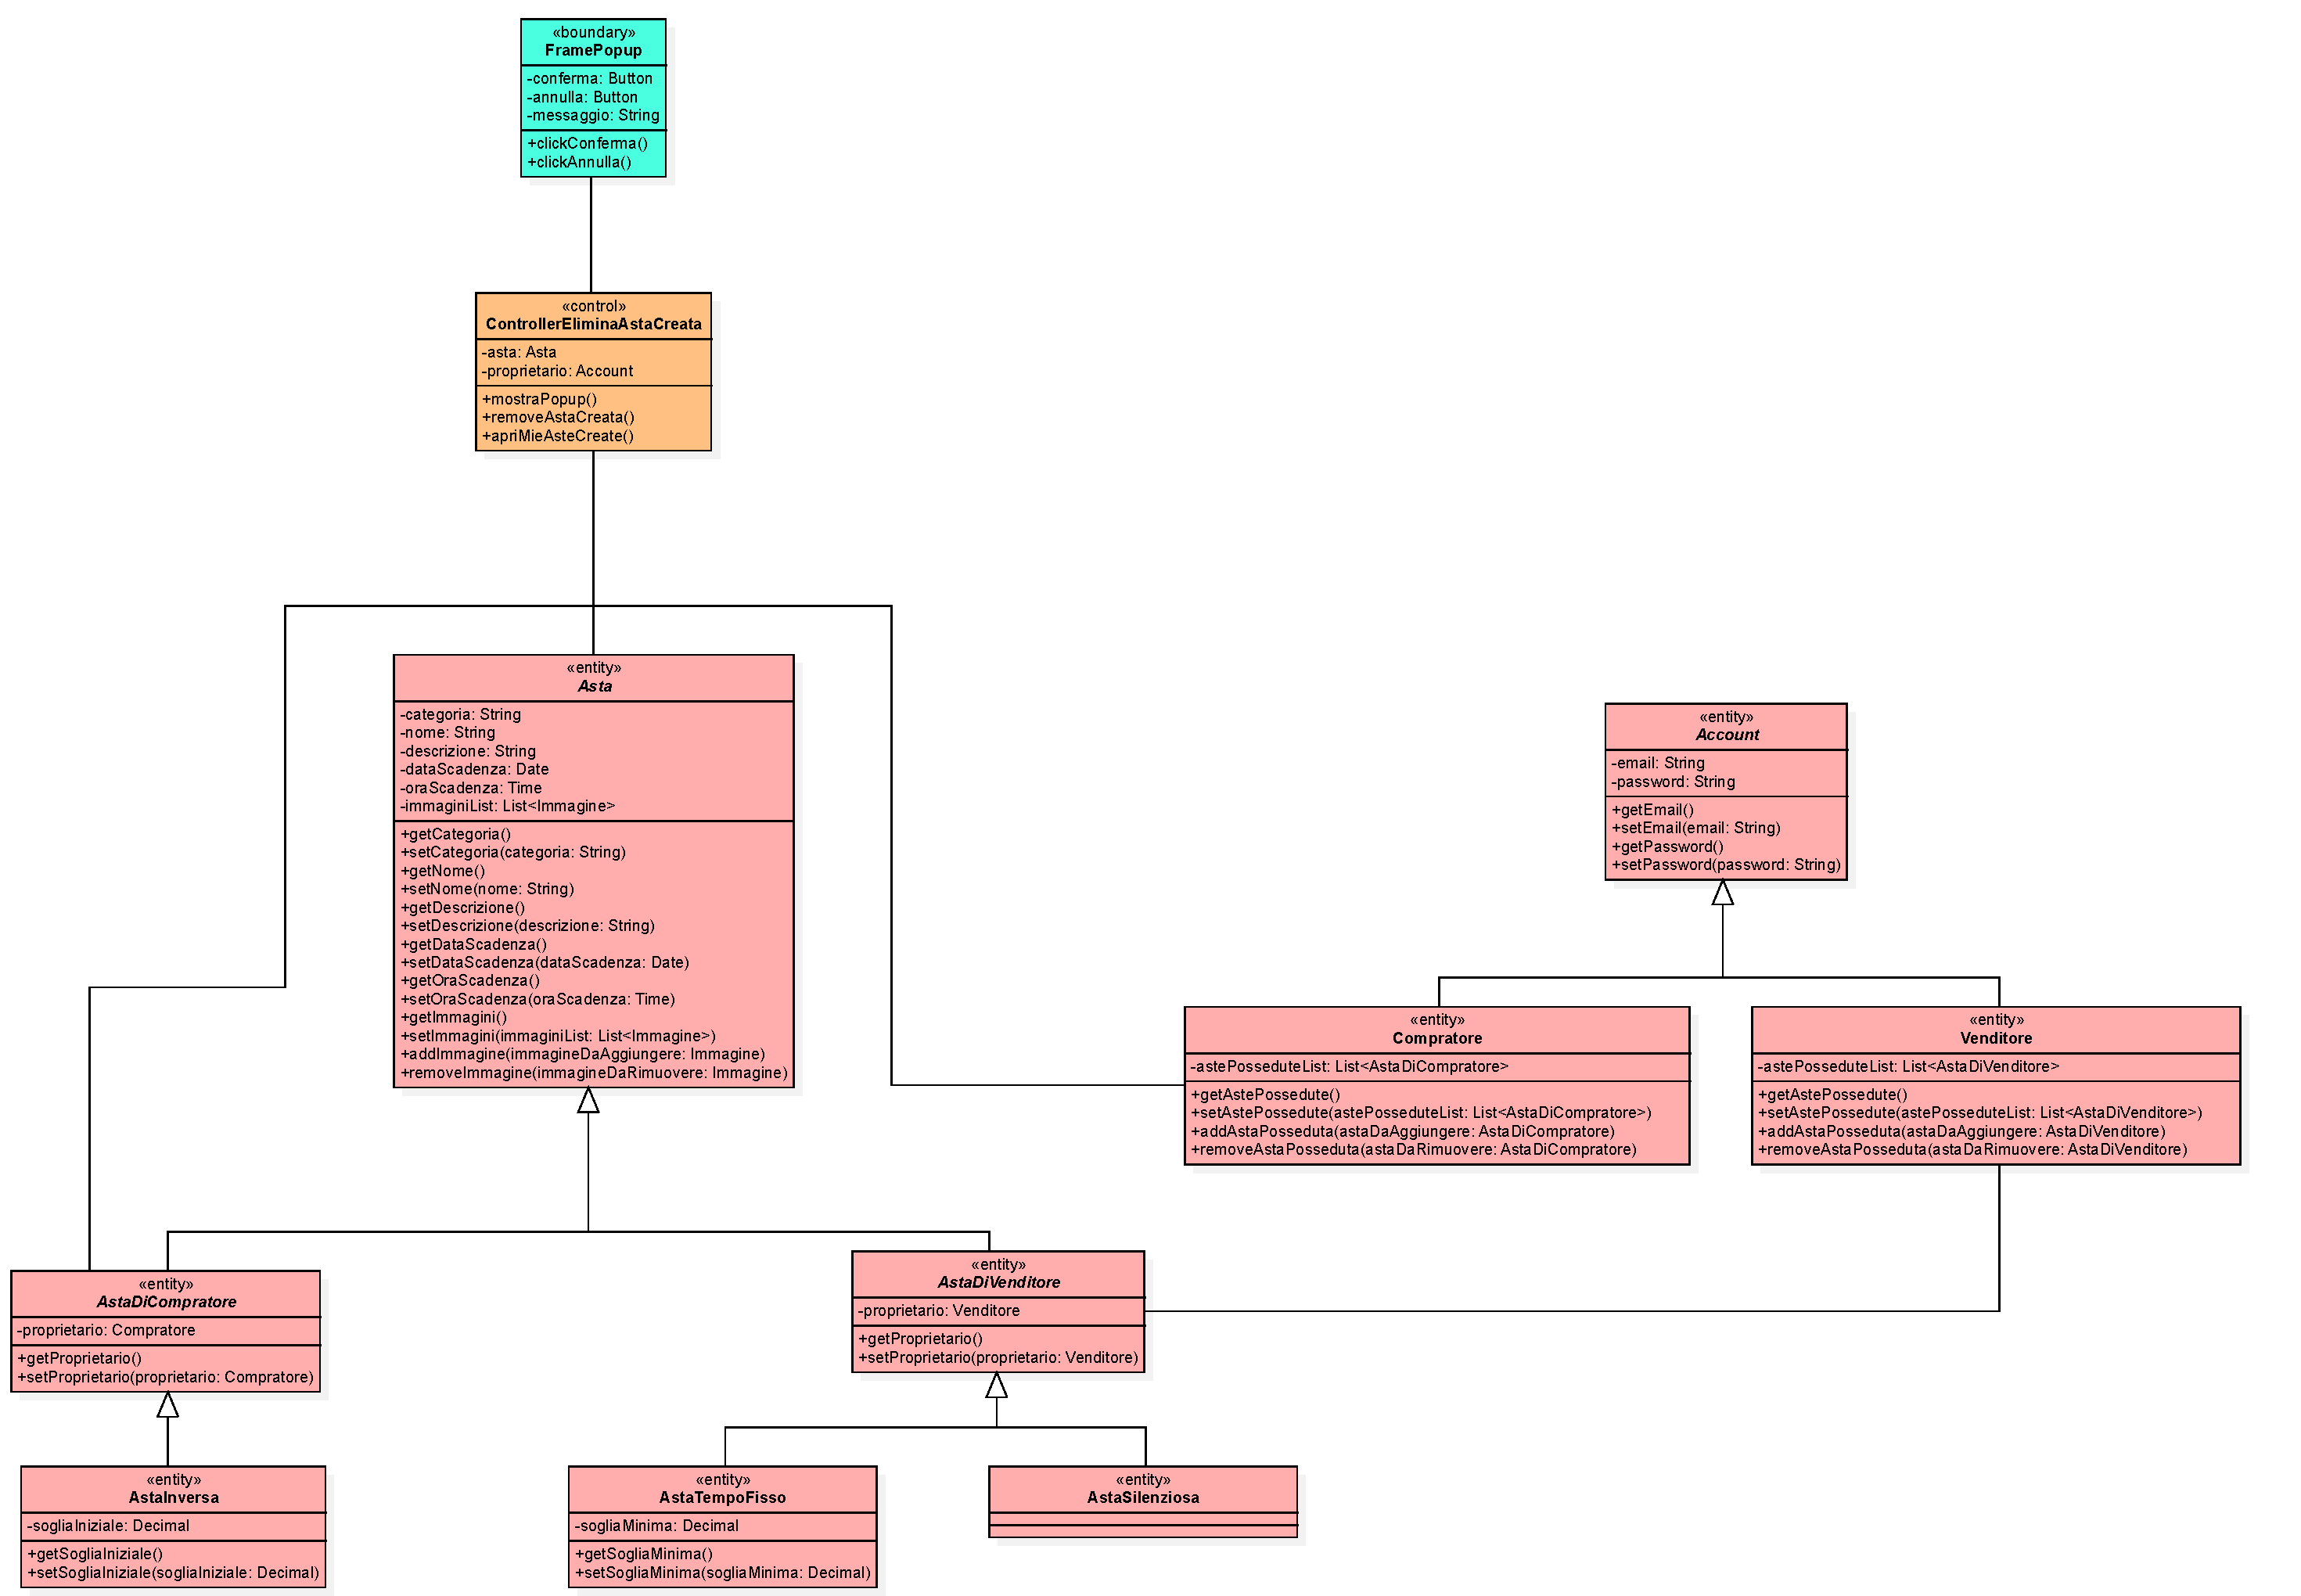
\includegraphics[width=1\linewidth]{Immagini/Diagrammi/Class Diagram/Utente che ha effettuato l'accesso/EliminaAsta.pdf}
                \caption{Elimina asta creata}
            \end{figure}
            
            \begin{figure}[htbp!]
                \centering
                    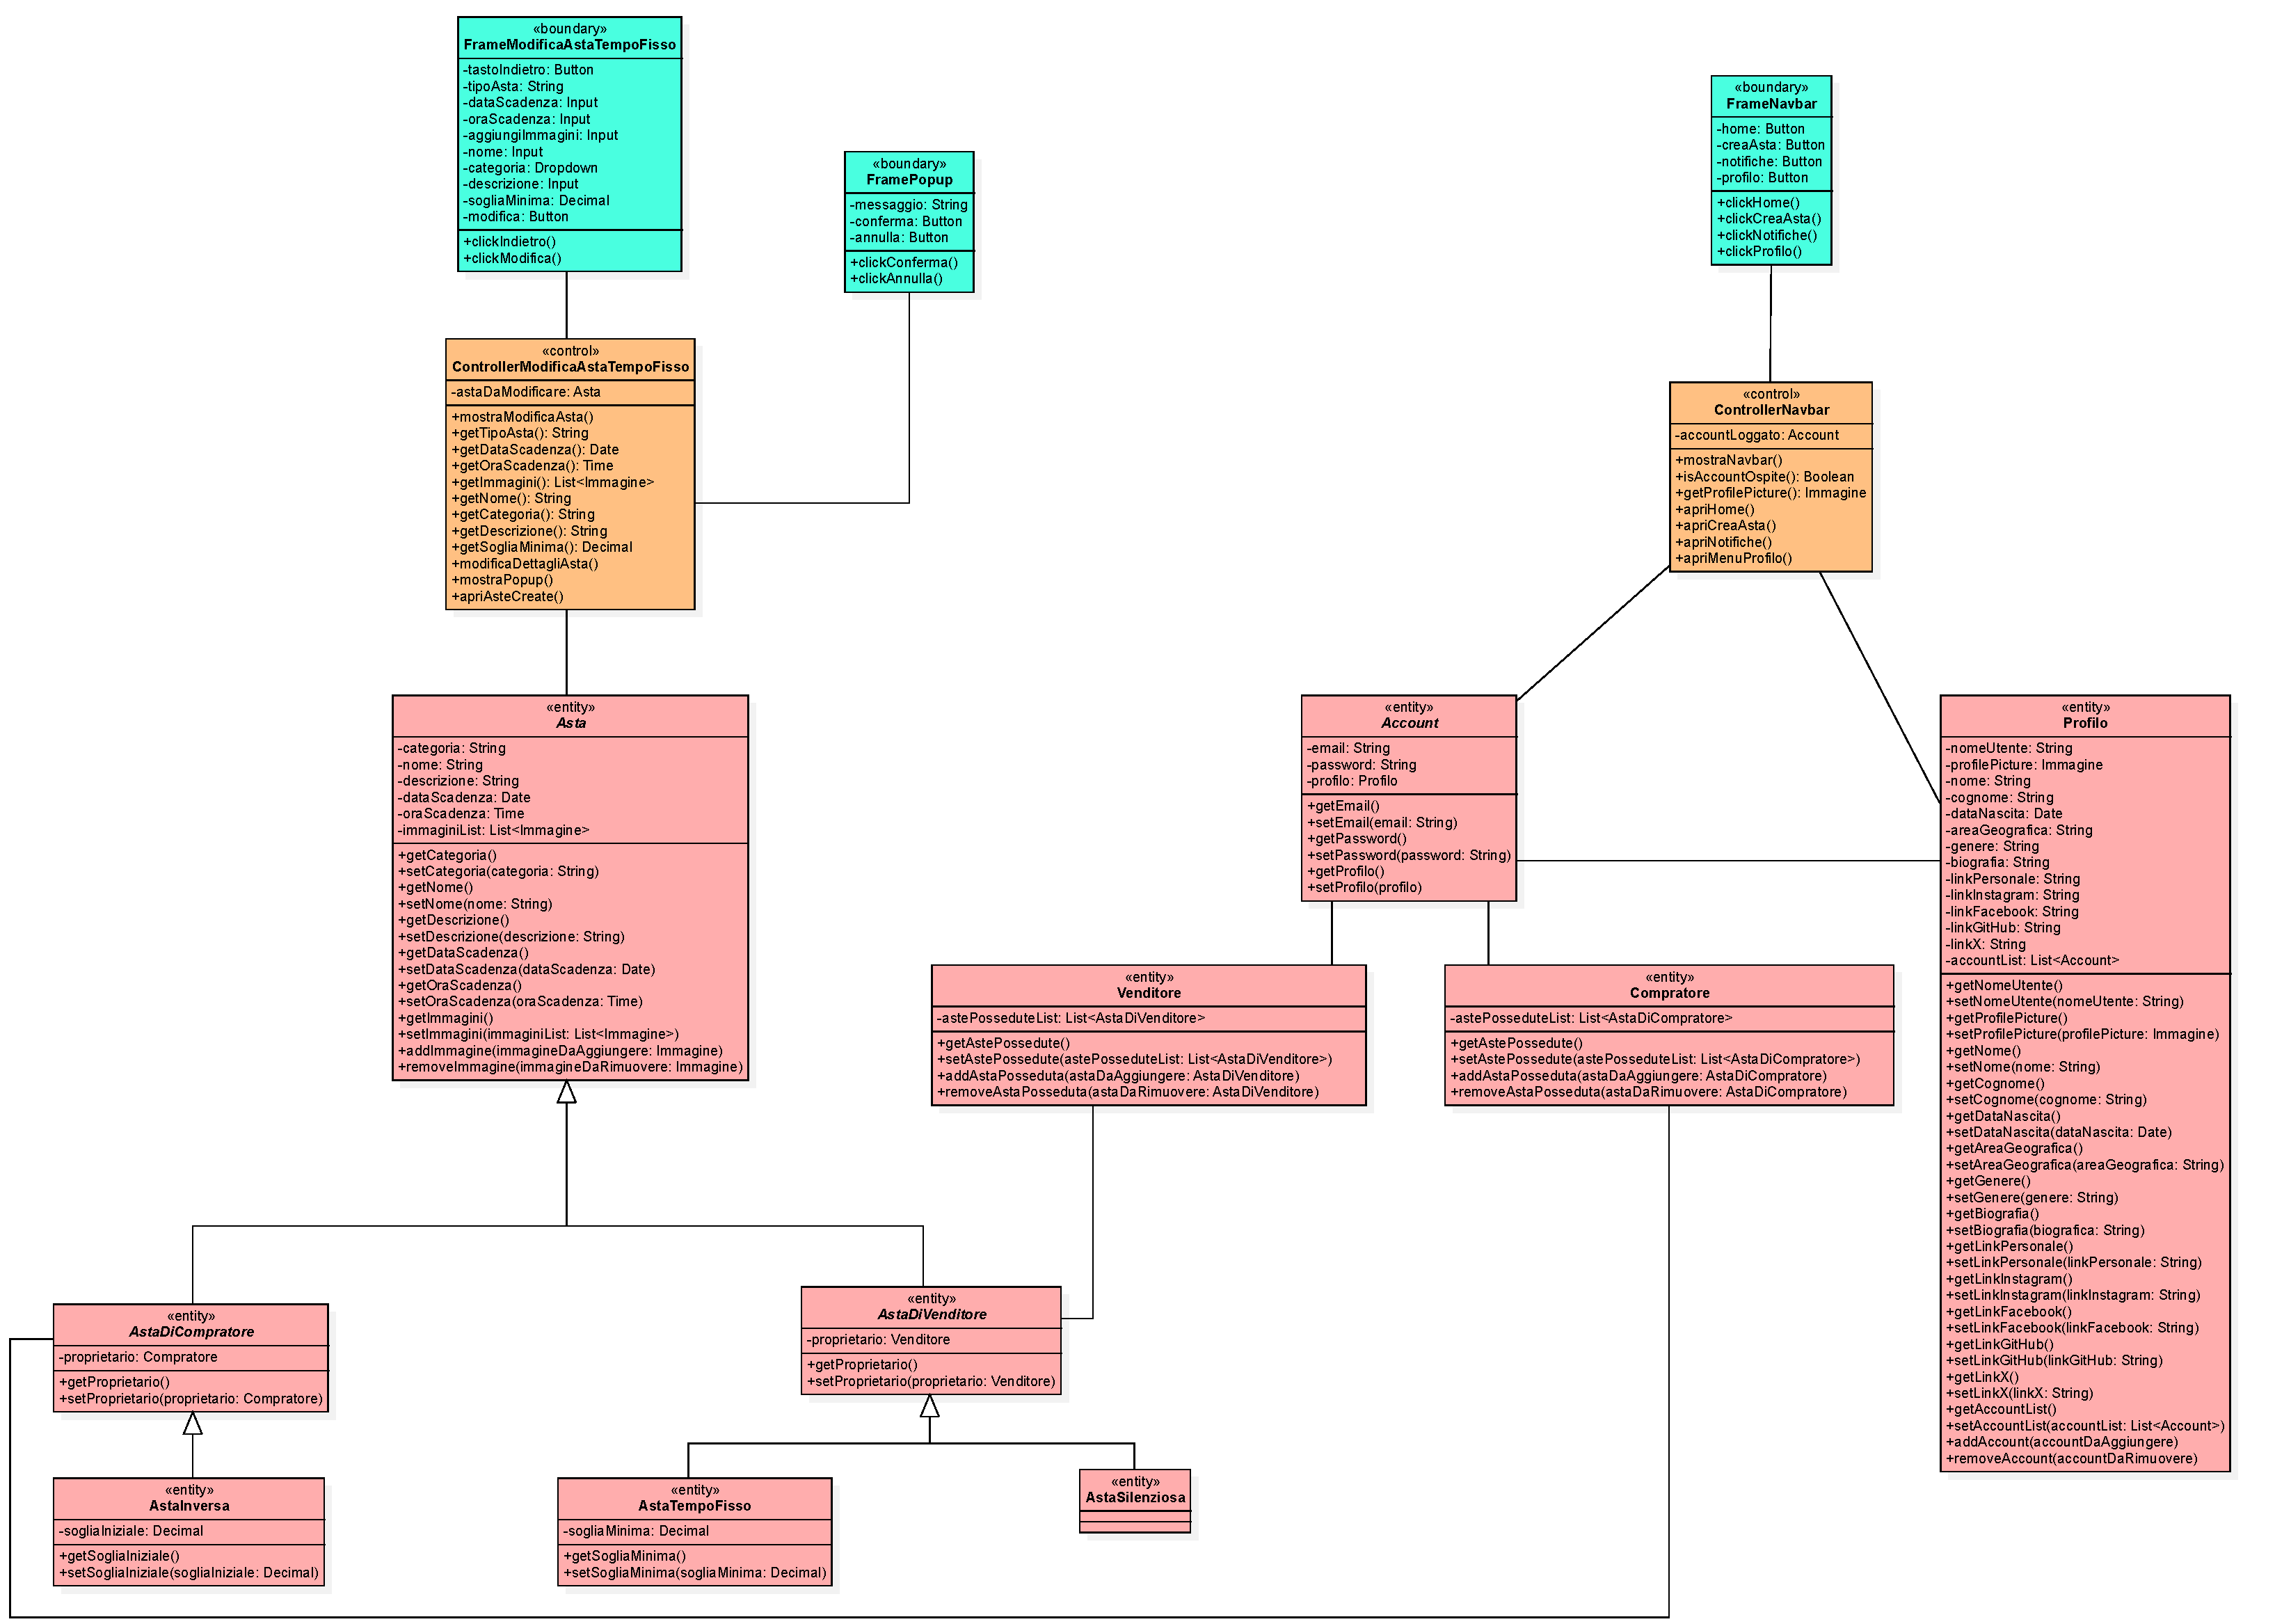
\includegraphics[width=1\linewidth]{Immagini/Diagrammi/Class Diagram/Utente che ha effettuato l'accesso/ModificaAstaTempoFisso.pdf}
                \caption{Modifica asta a tempo fisso}
            \end{figure}
            
            \begin{figure}[htbp!]
                \centering
                    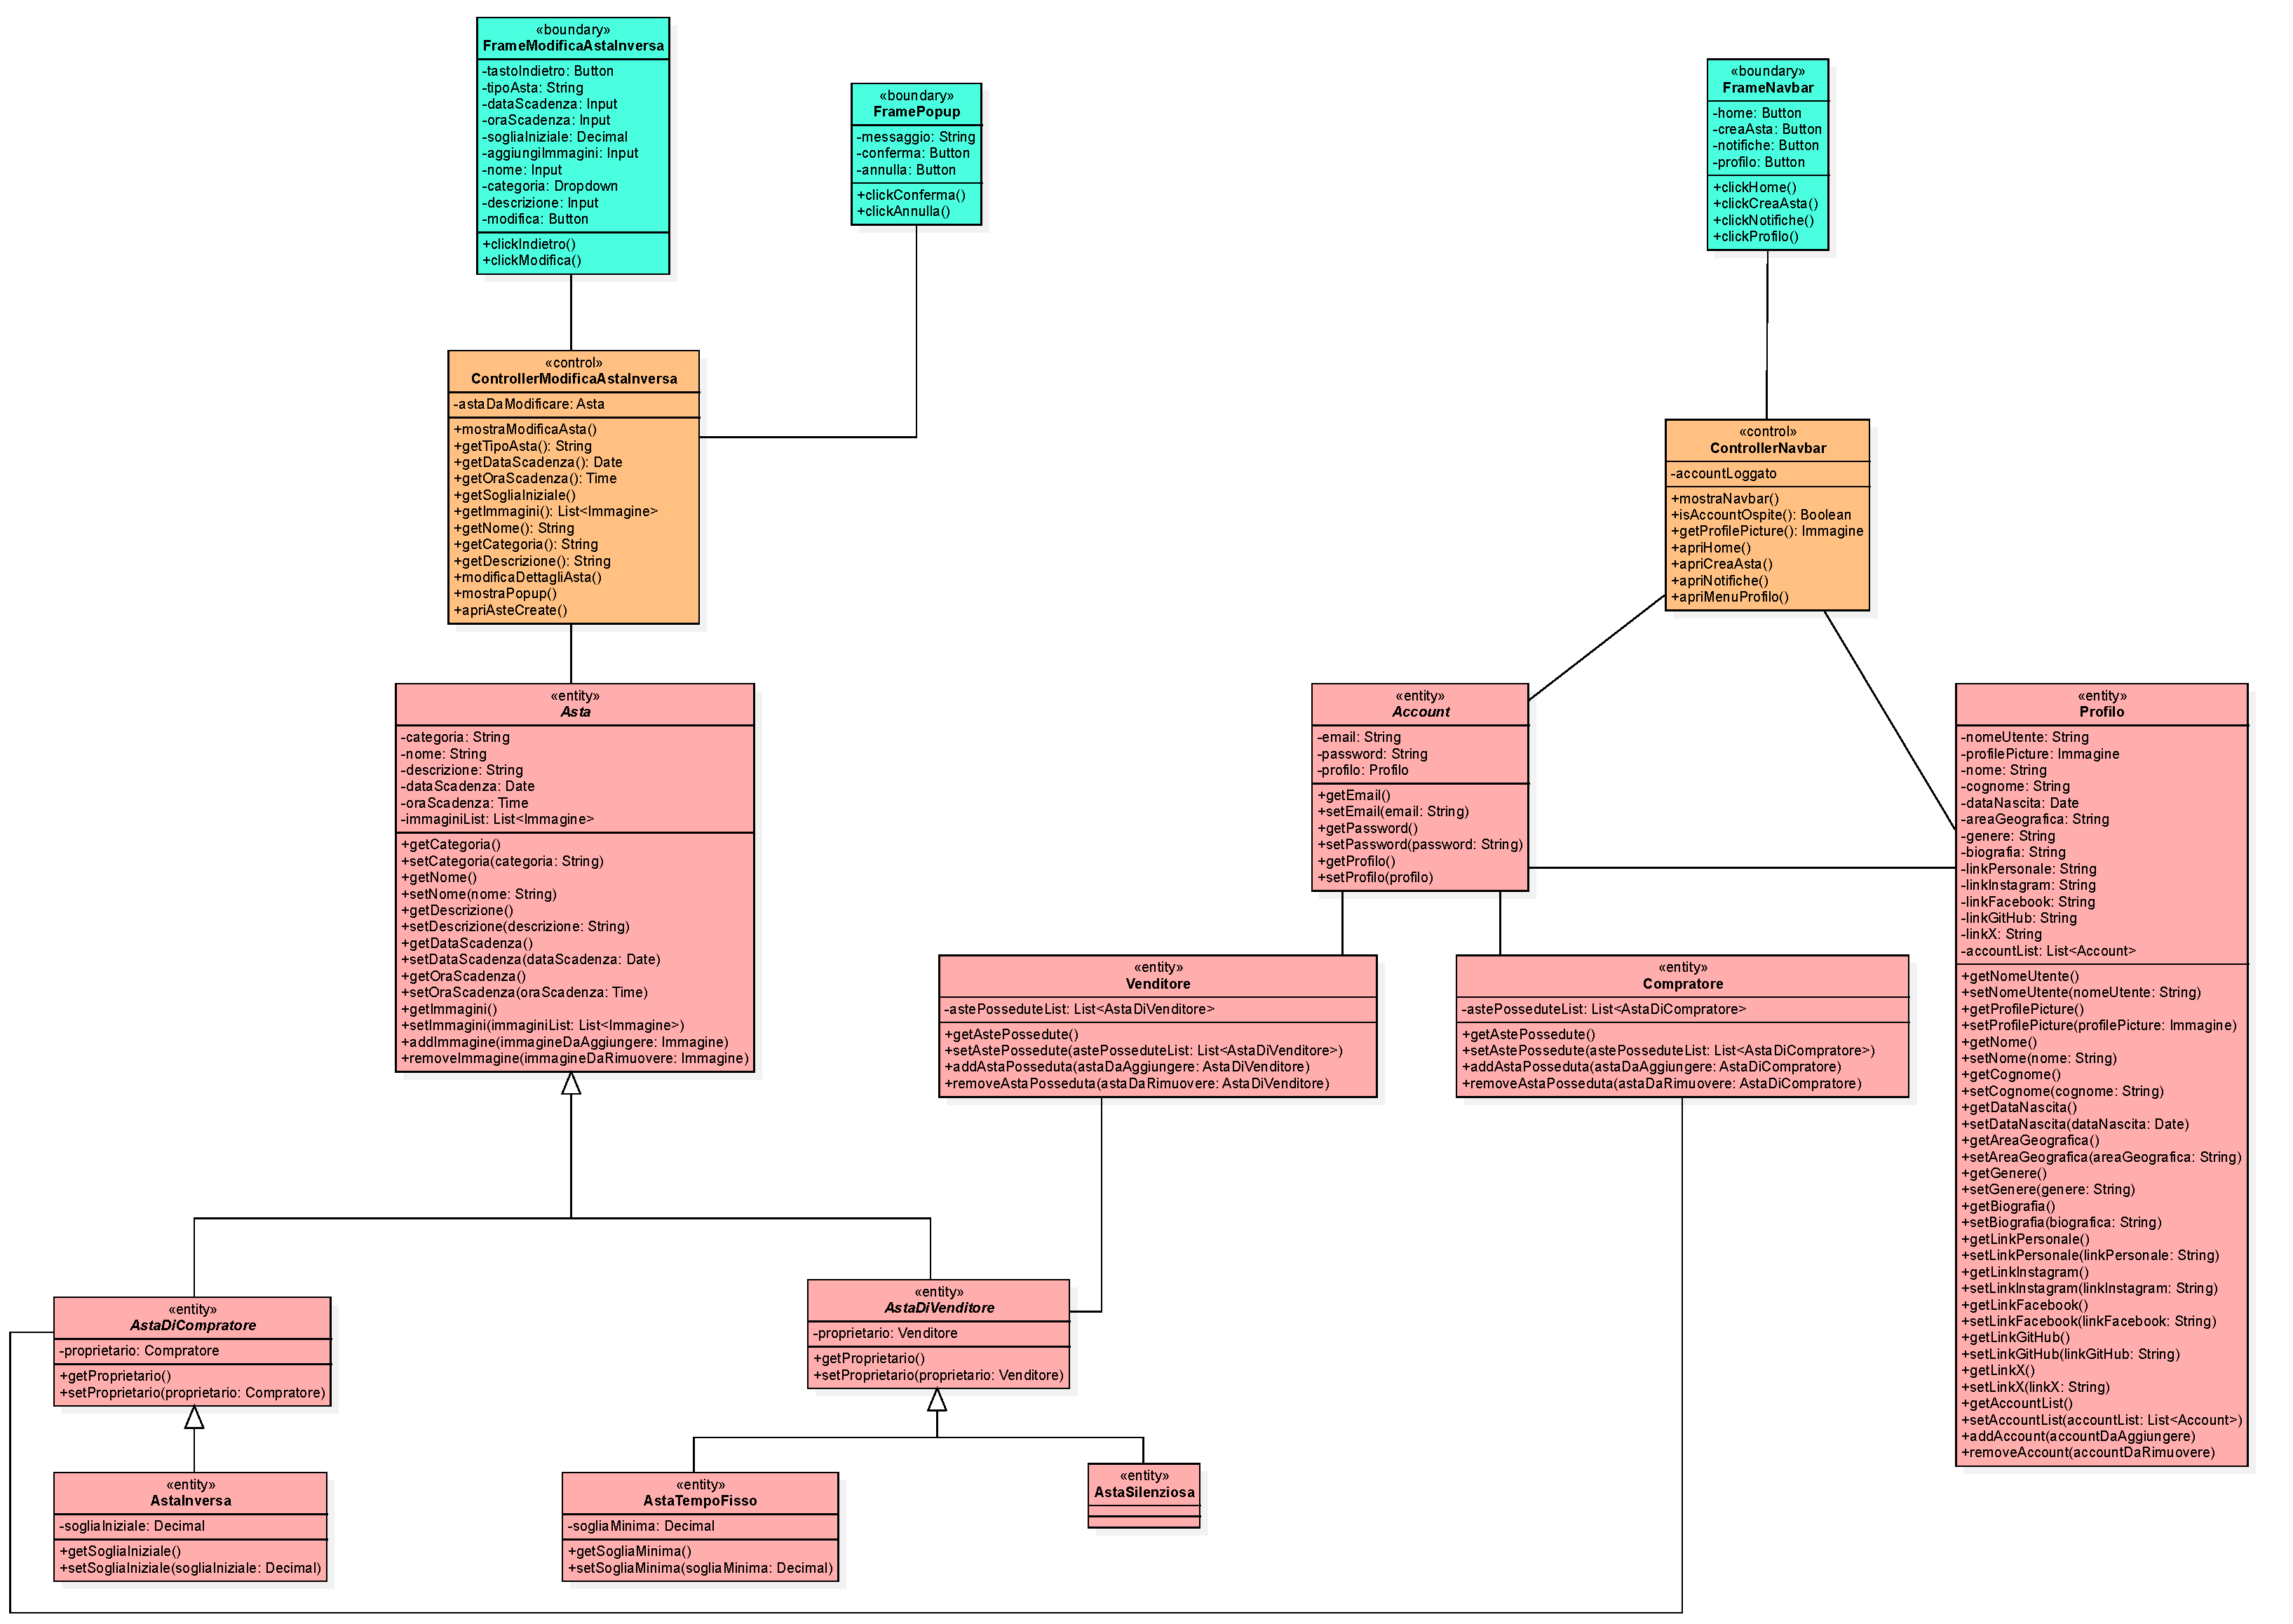
\includegraphics[width=1\linewidth]{Immagini/Diagrammi/Class Diagram/Utente che ha effettuato l'accesso/ModificaAstaInversa.pdf}
                \caption{Modifica asta inversa}
            \end{figure}
            
            \begin{figure}[htbp!]
                \centering
                    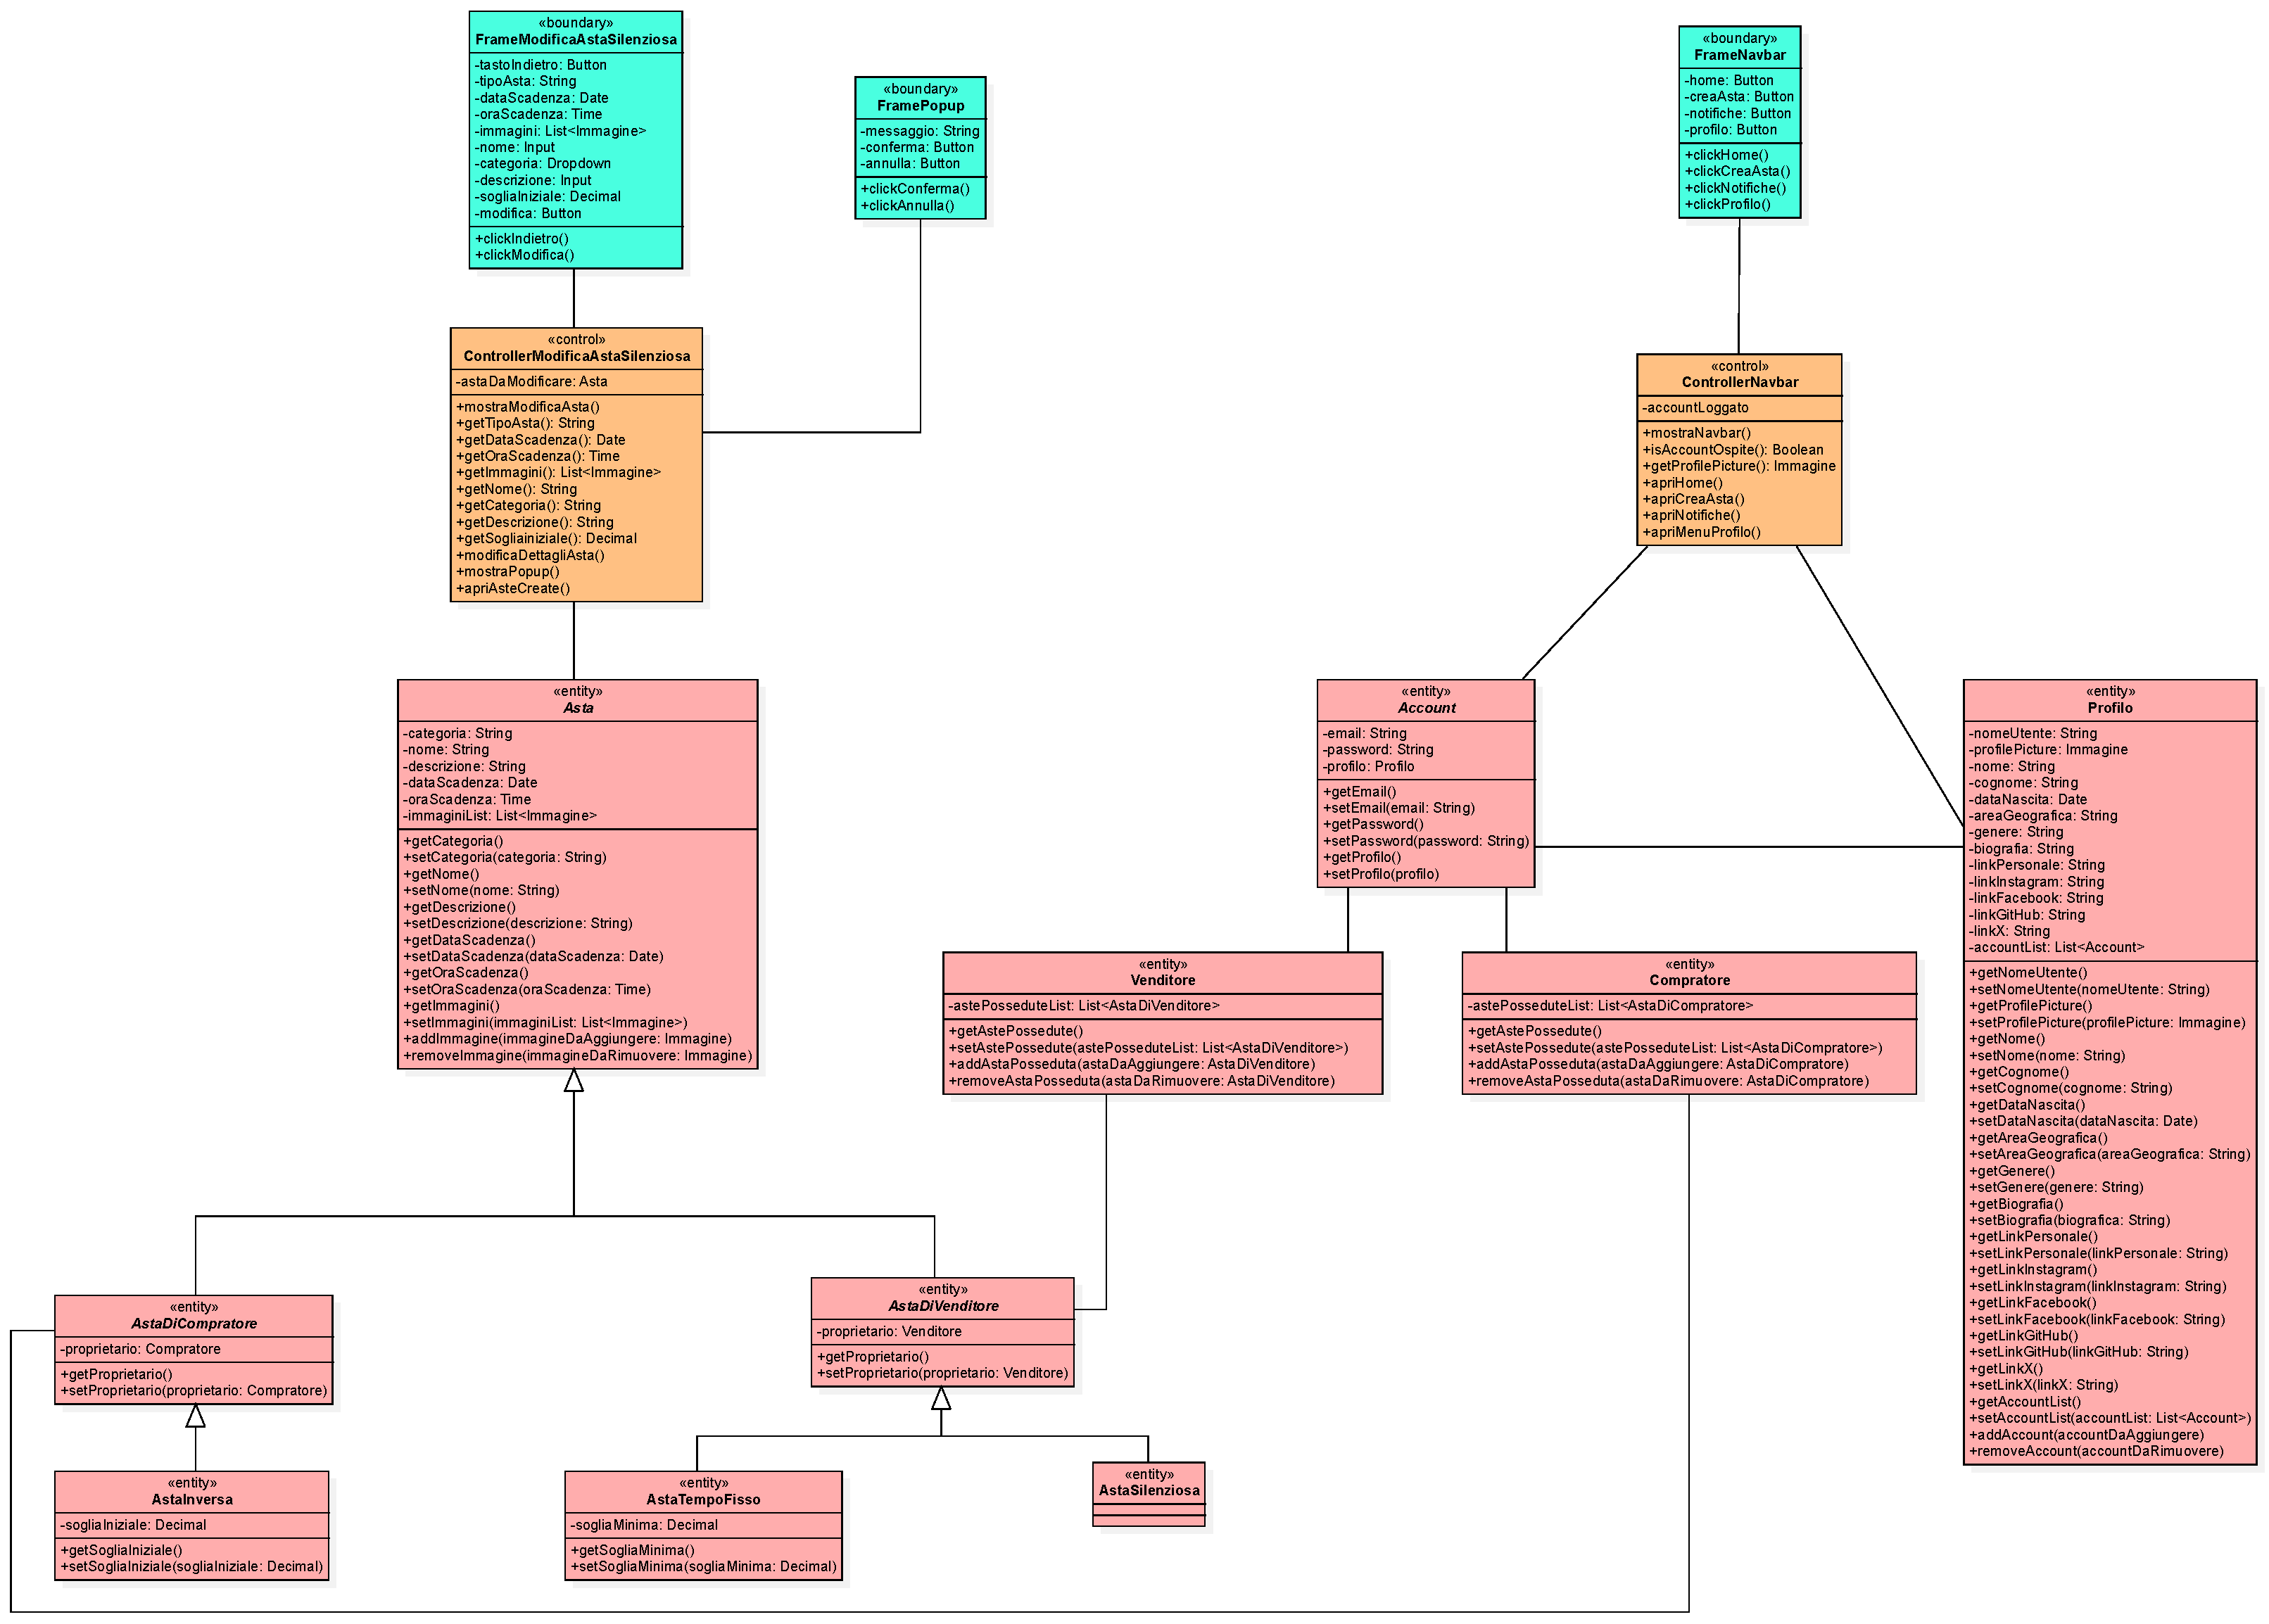
\includegraphics[width=1\linewidth]{Immagini/Diagrammi/Class Diagram/Utente che ha effettuato l'accesso/ModificaAstaSilenziosa.pdf}
                \caption{Modifica asta silenziosa}
            \end{figure}
            
            \begin{figure}[htbp!]
                \centering
                    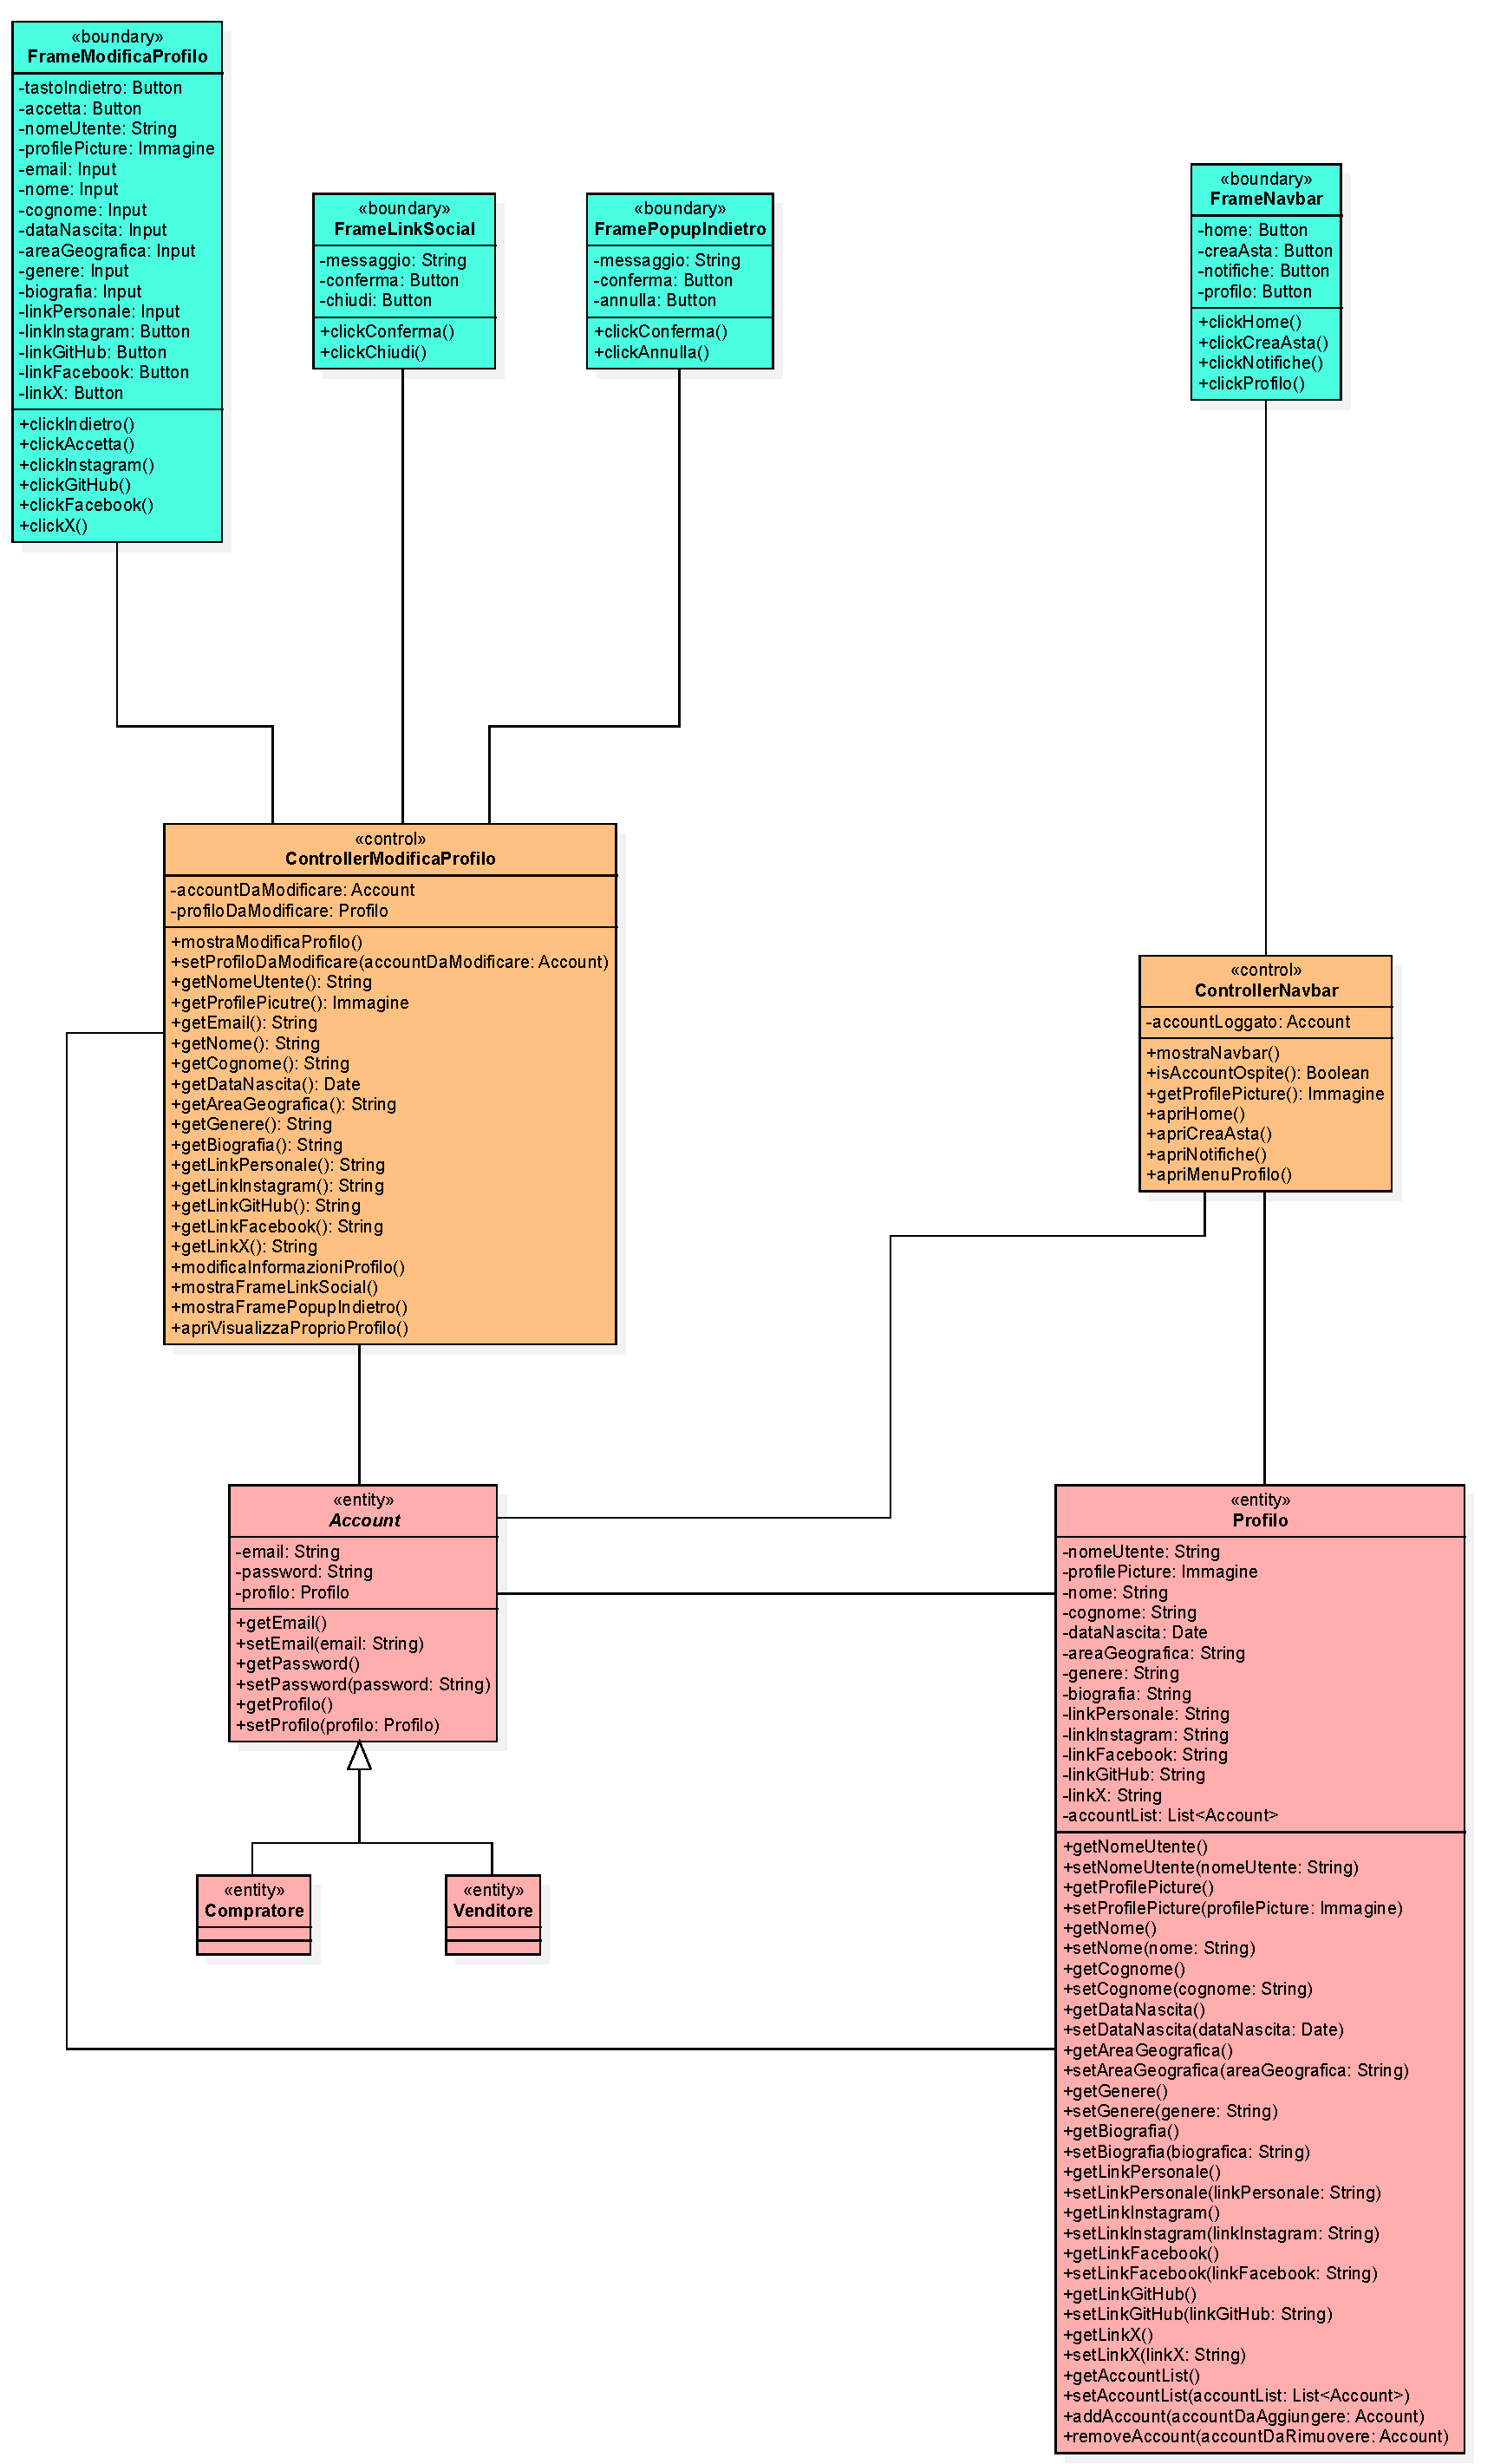
\includegraphics[width=0.8\linewidth]{Immagini/Diagrammi/Class Diagram/Utente che ha effettuato l'accesso/ModificaProfilo.pdf}
                \caption{Modifica profilo}
            \end{figure}

            \begin{figure}[htbp!]
                \centering
                    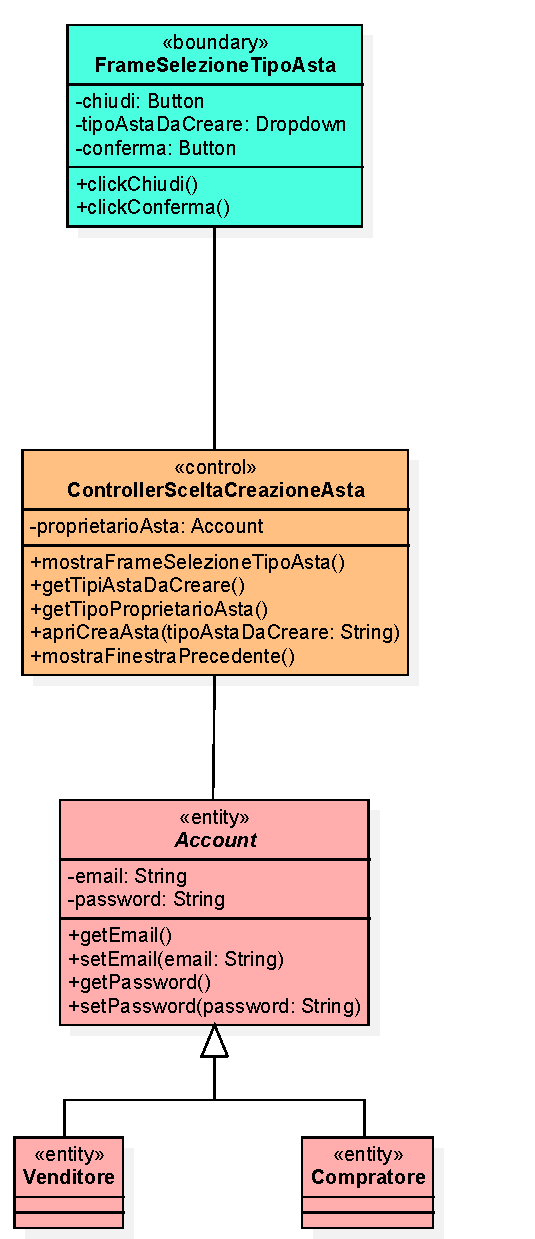
\includegraphics[width=0.5\linewidth]{Immagini/Diagrammi/Class Diagram/Utente che ha effettuato l'accesso/SceltaCreazioneAsta.pdf}
                \caption{Scelta tipo di asta da creare}
            \end{figure}
            
            \begin{figure}[htbp!]
                \centering
                    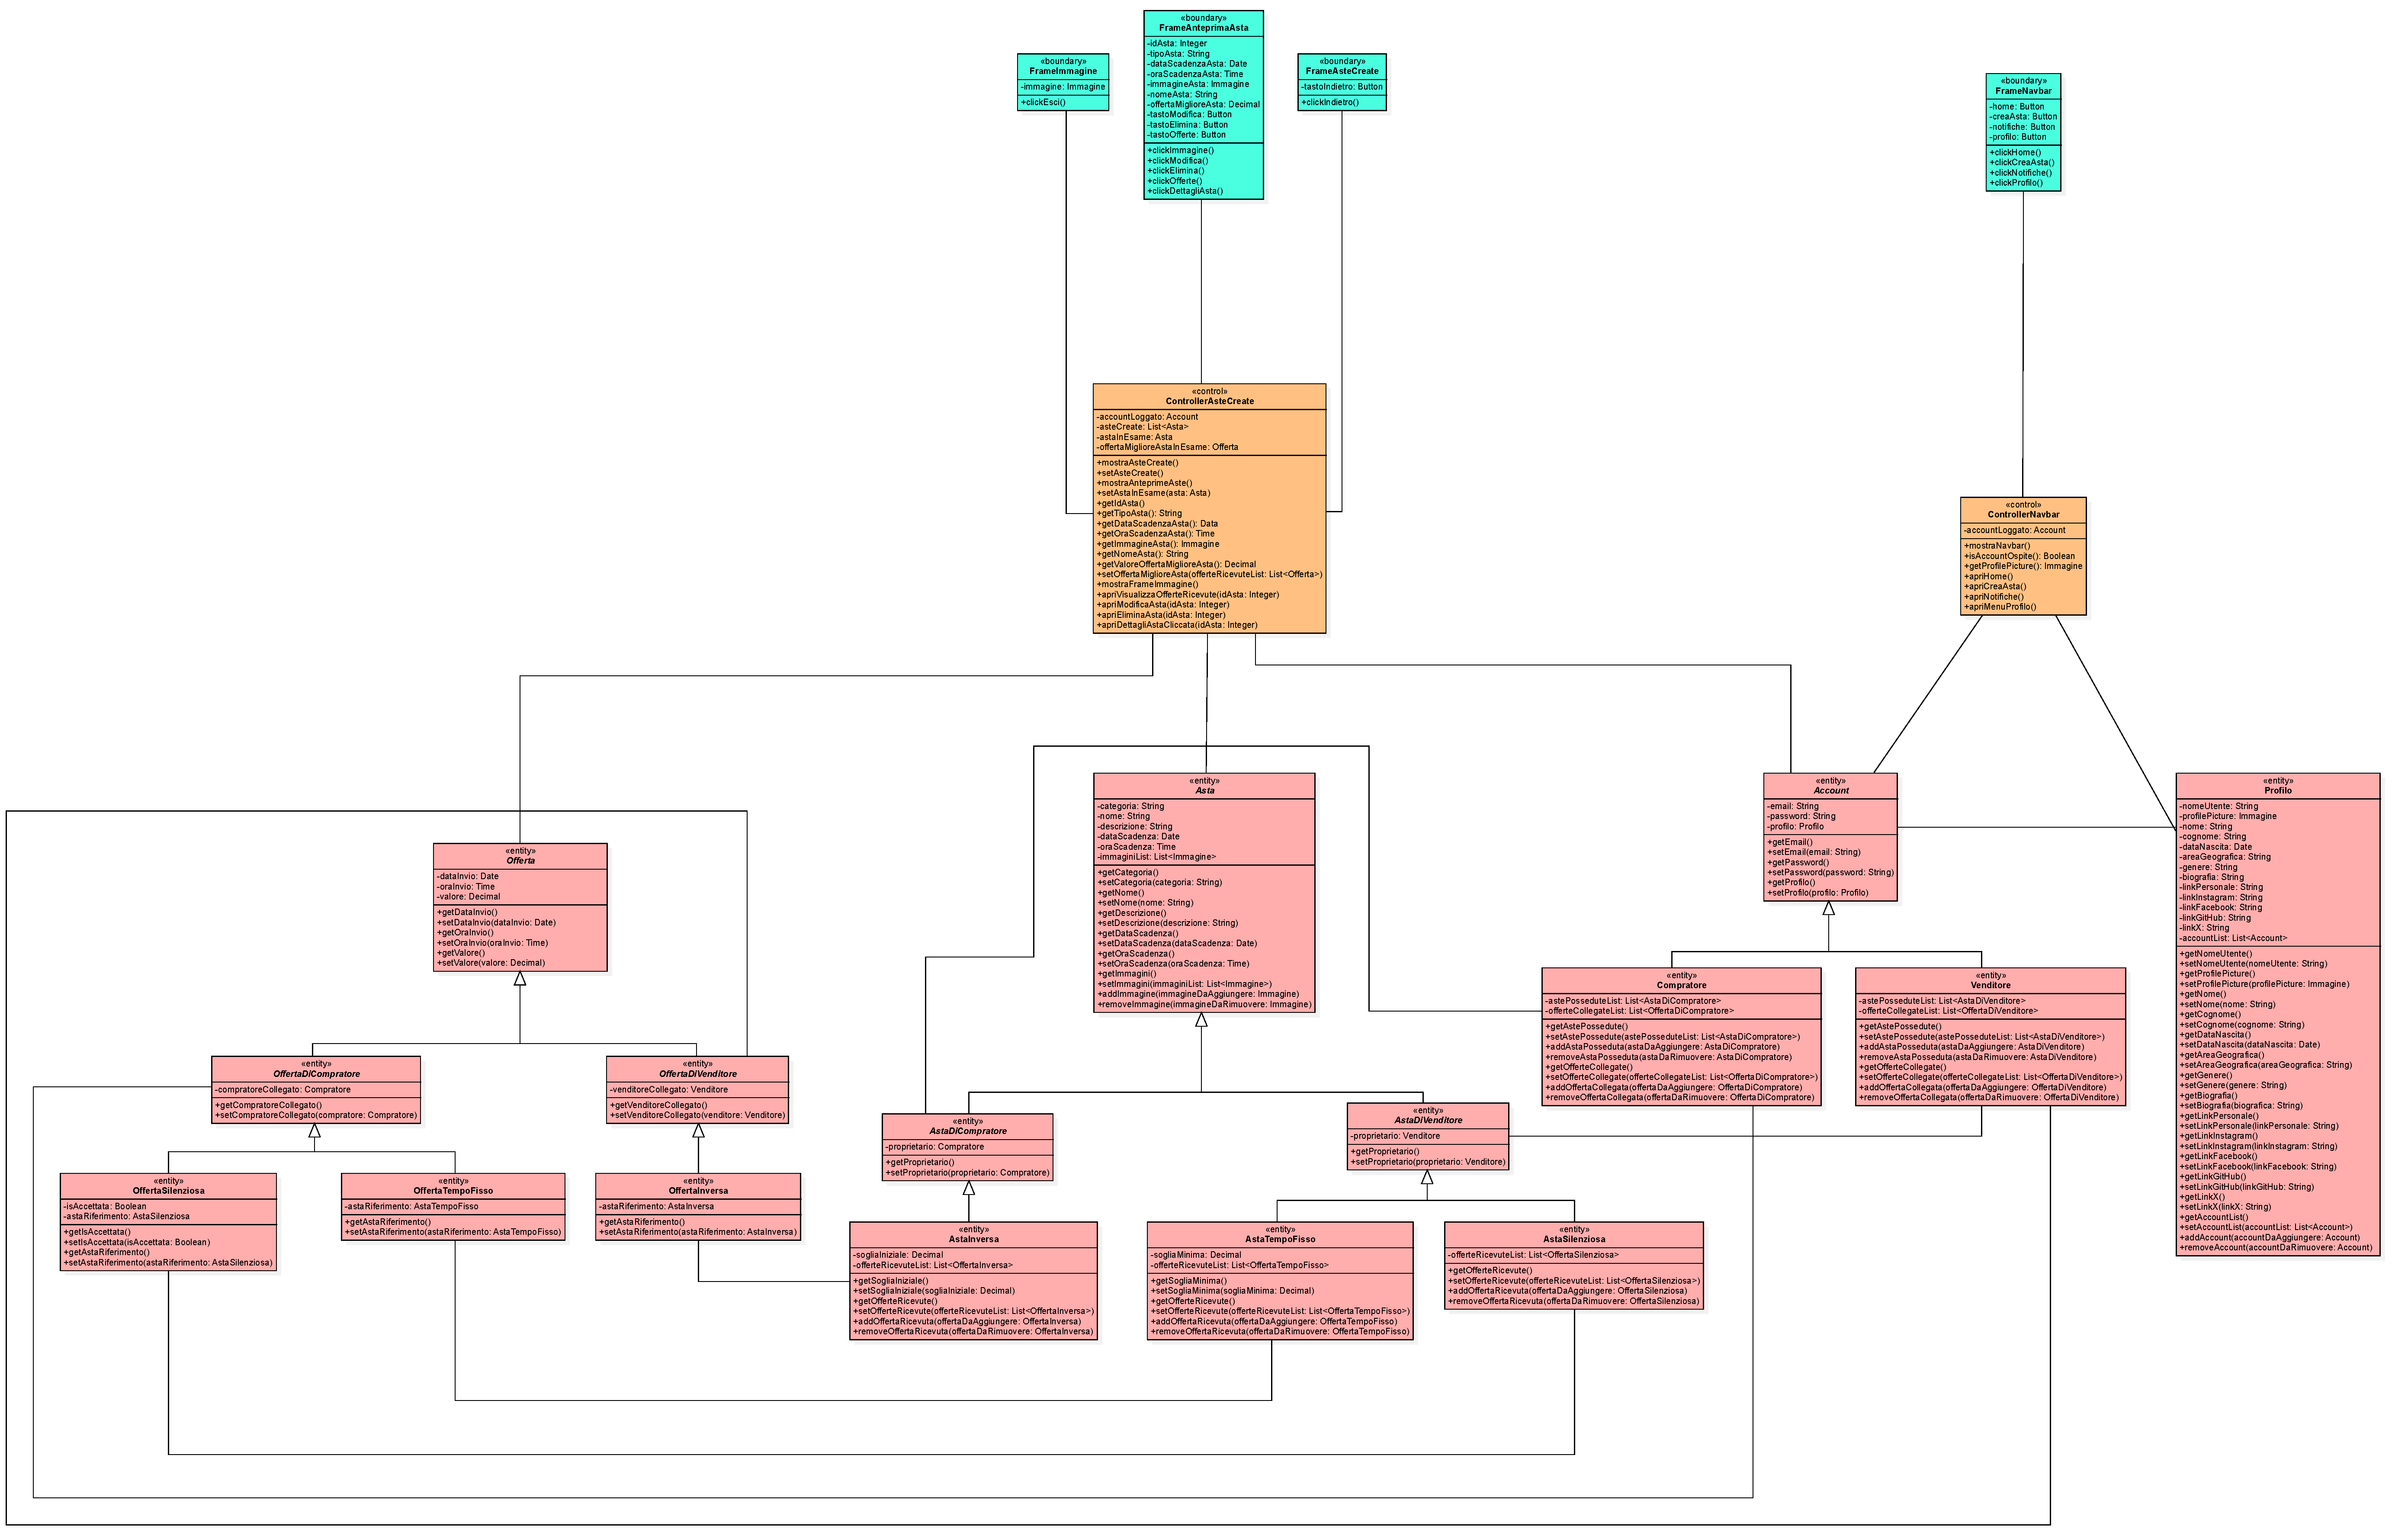
\includegraphics[width=1\linewidth]{Immagini/Diagrammi/Class Diagram/Utente che ha effettuato l'accesso/VisualizzaAsteCreate.pdf}
                \caption{Visualizza aste create}
            \end{figure}

            \begin{figure}[htbp!]
                \centering
                    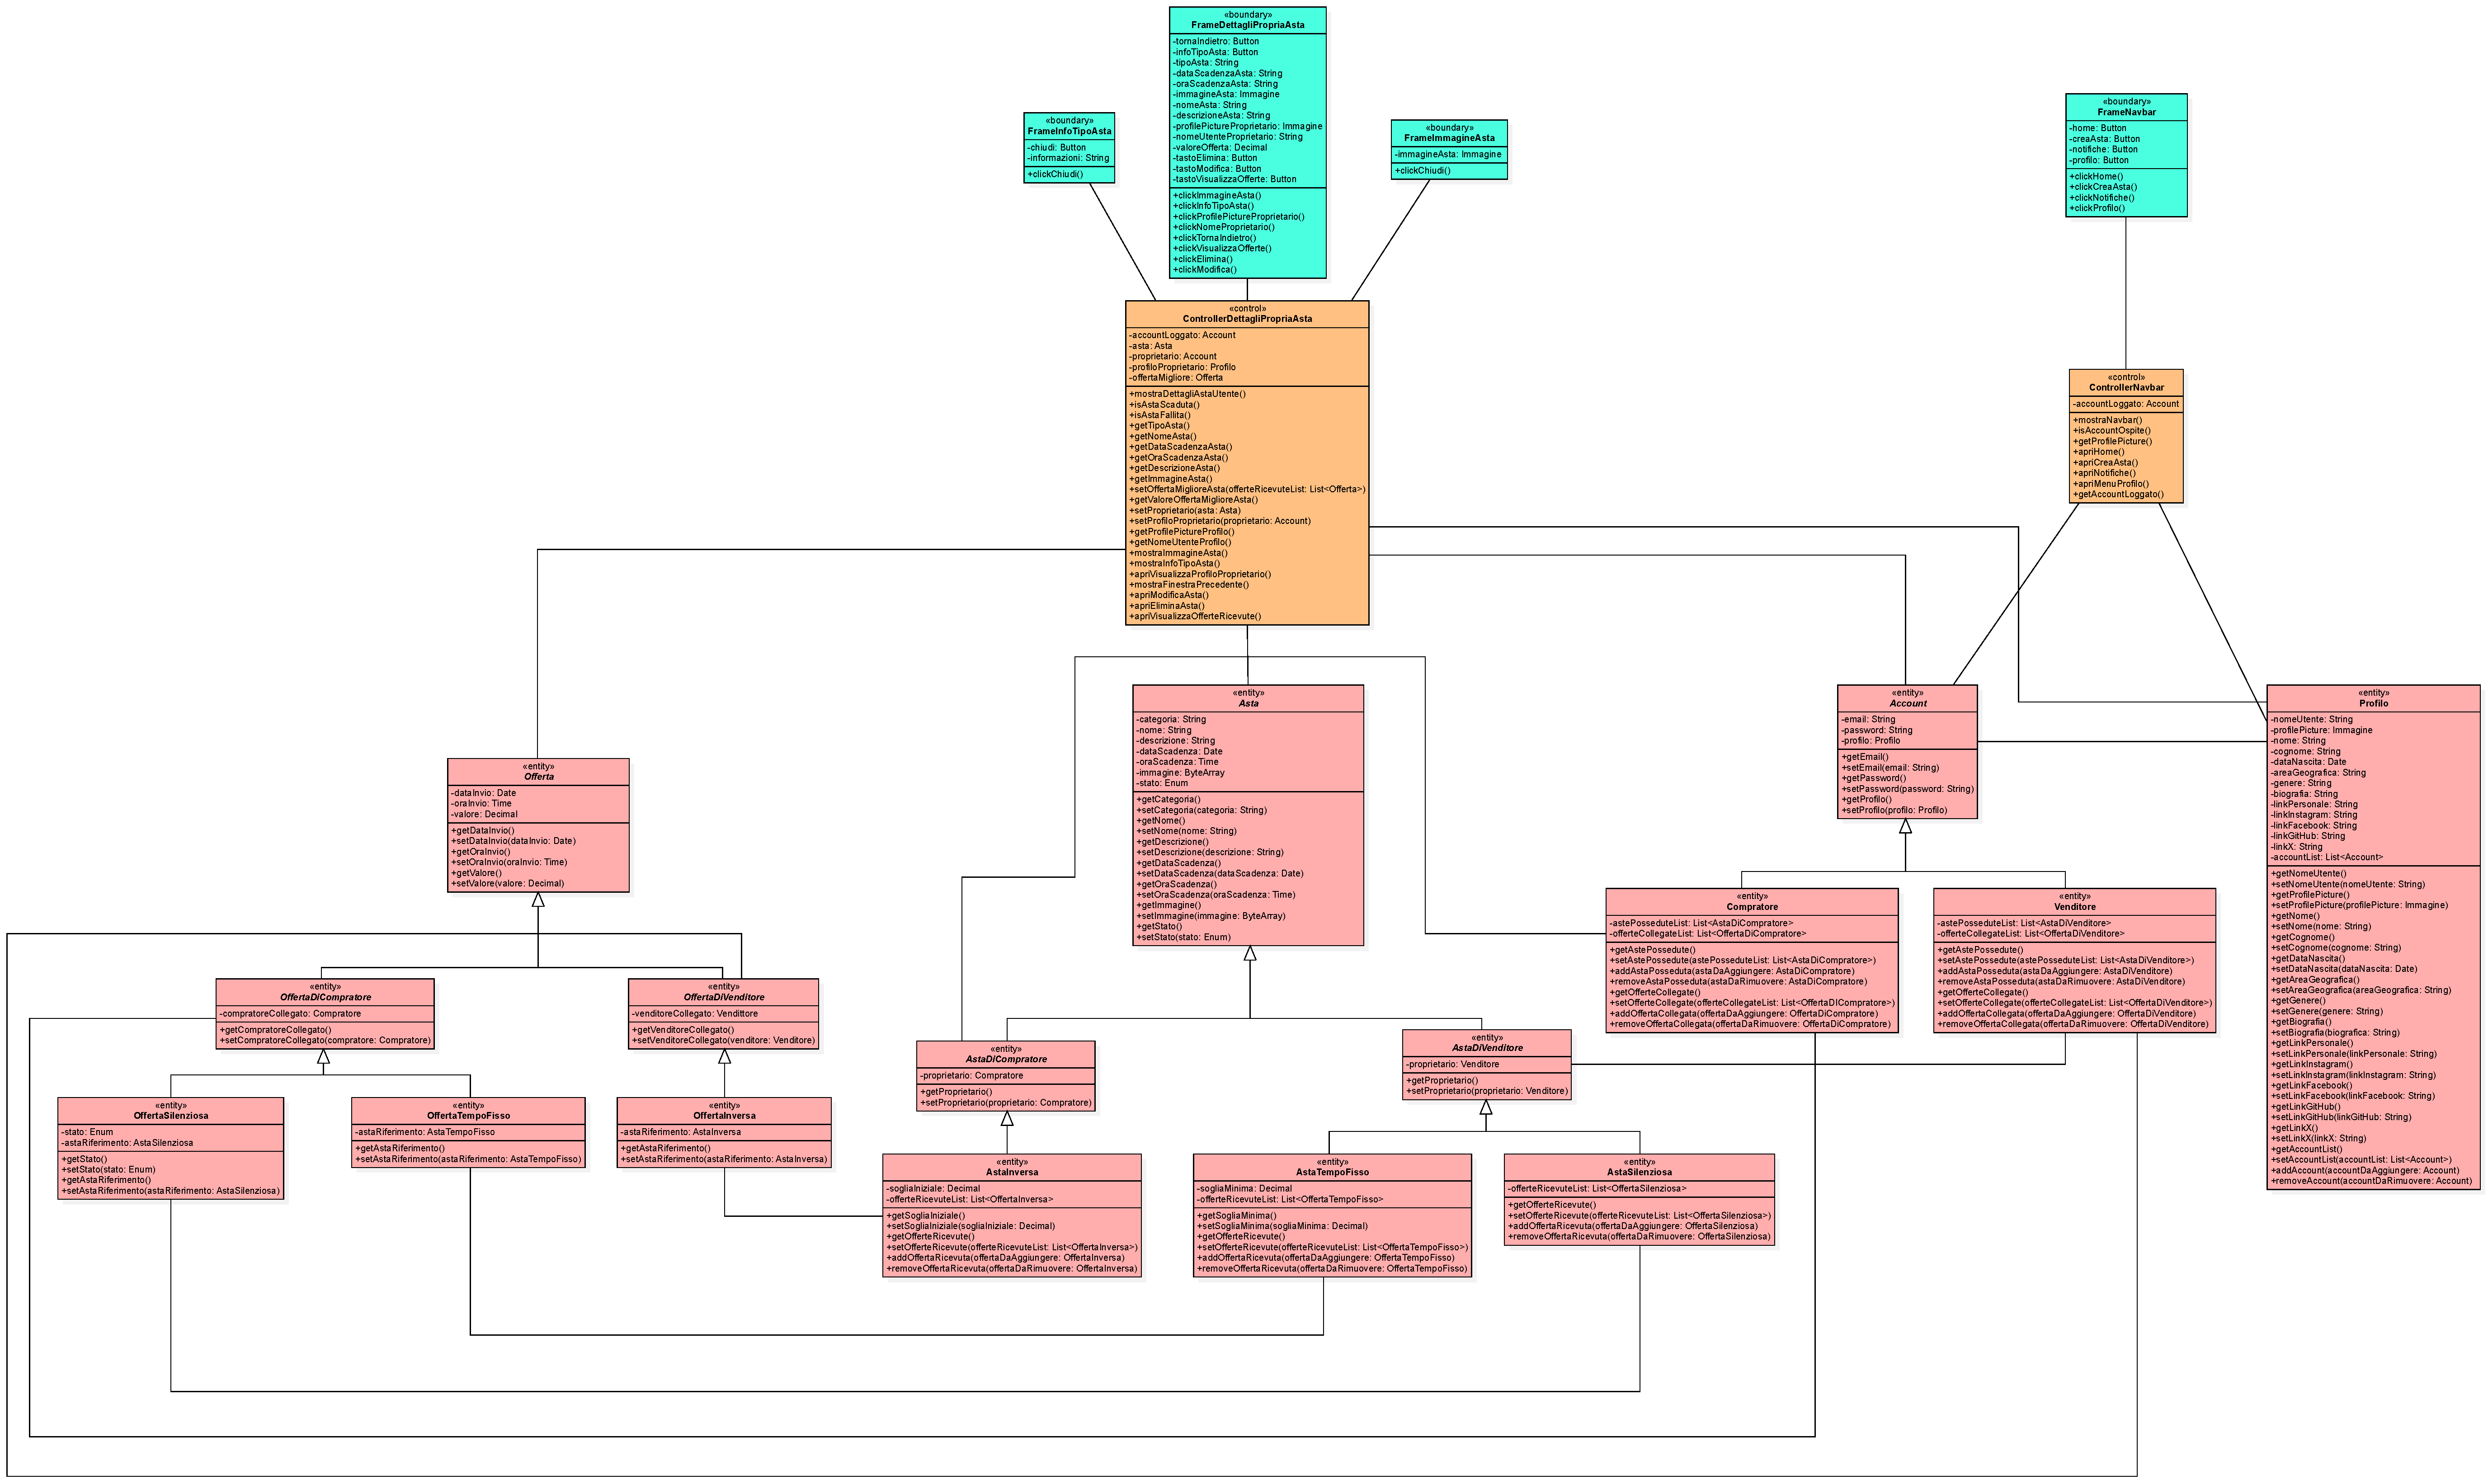
\includegraphics[width=1\linewidth]{Immagini/Diagrammi/Class Diagram/Utente che ha effettuato l'accesso/VisualizzaDettagliPropriaAsta.pdf}
                \caption{Visualizza dettagli della propria asta}
            \end{figure}
            
            \begin{figure}[htbp!]
                \centering
                    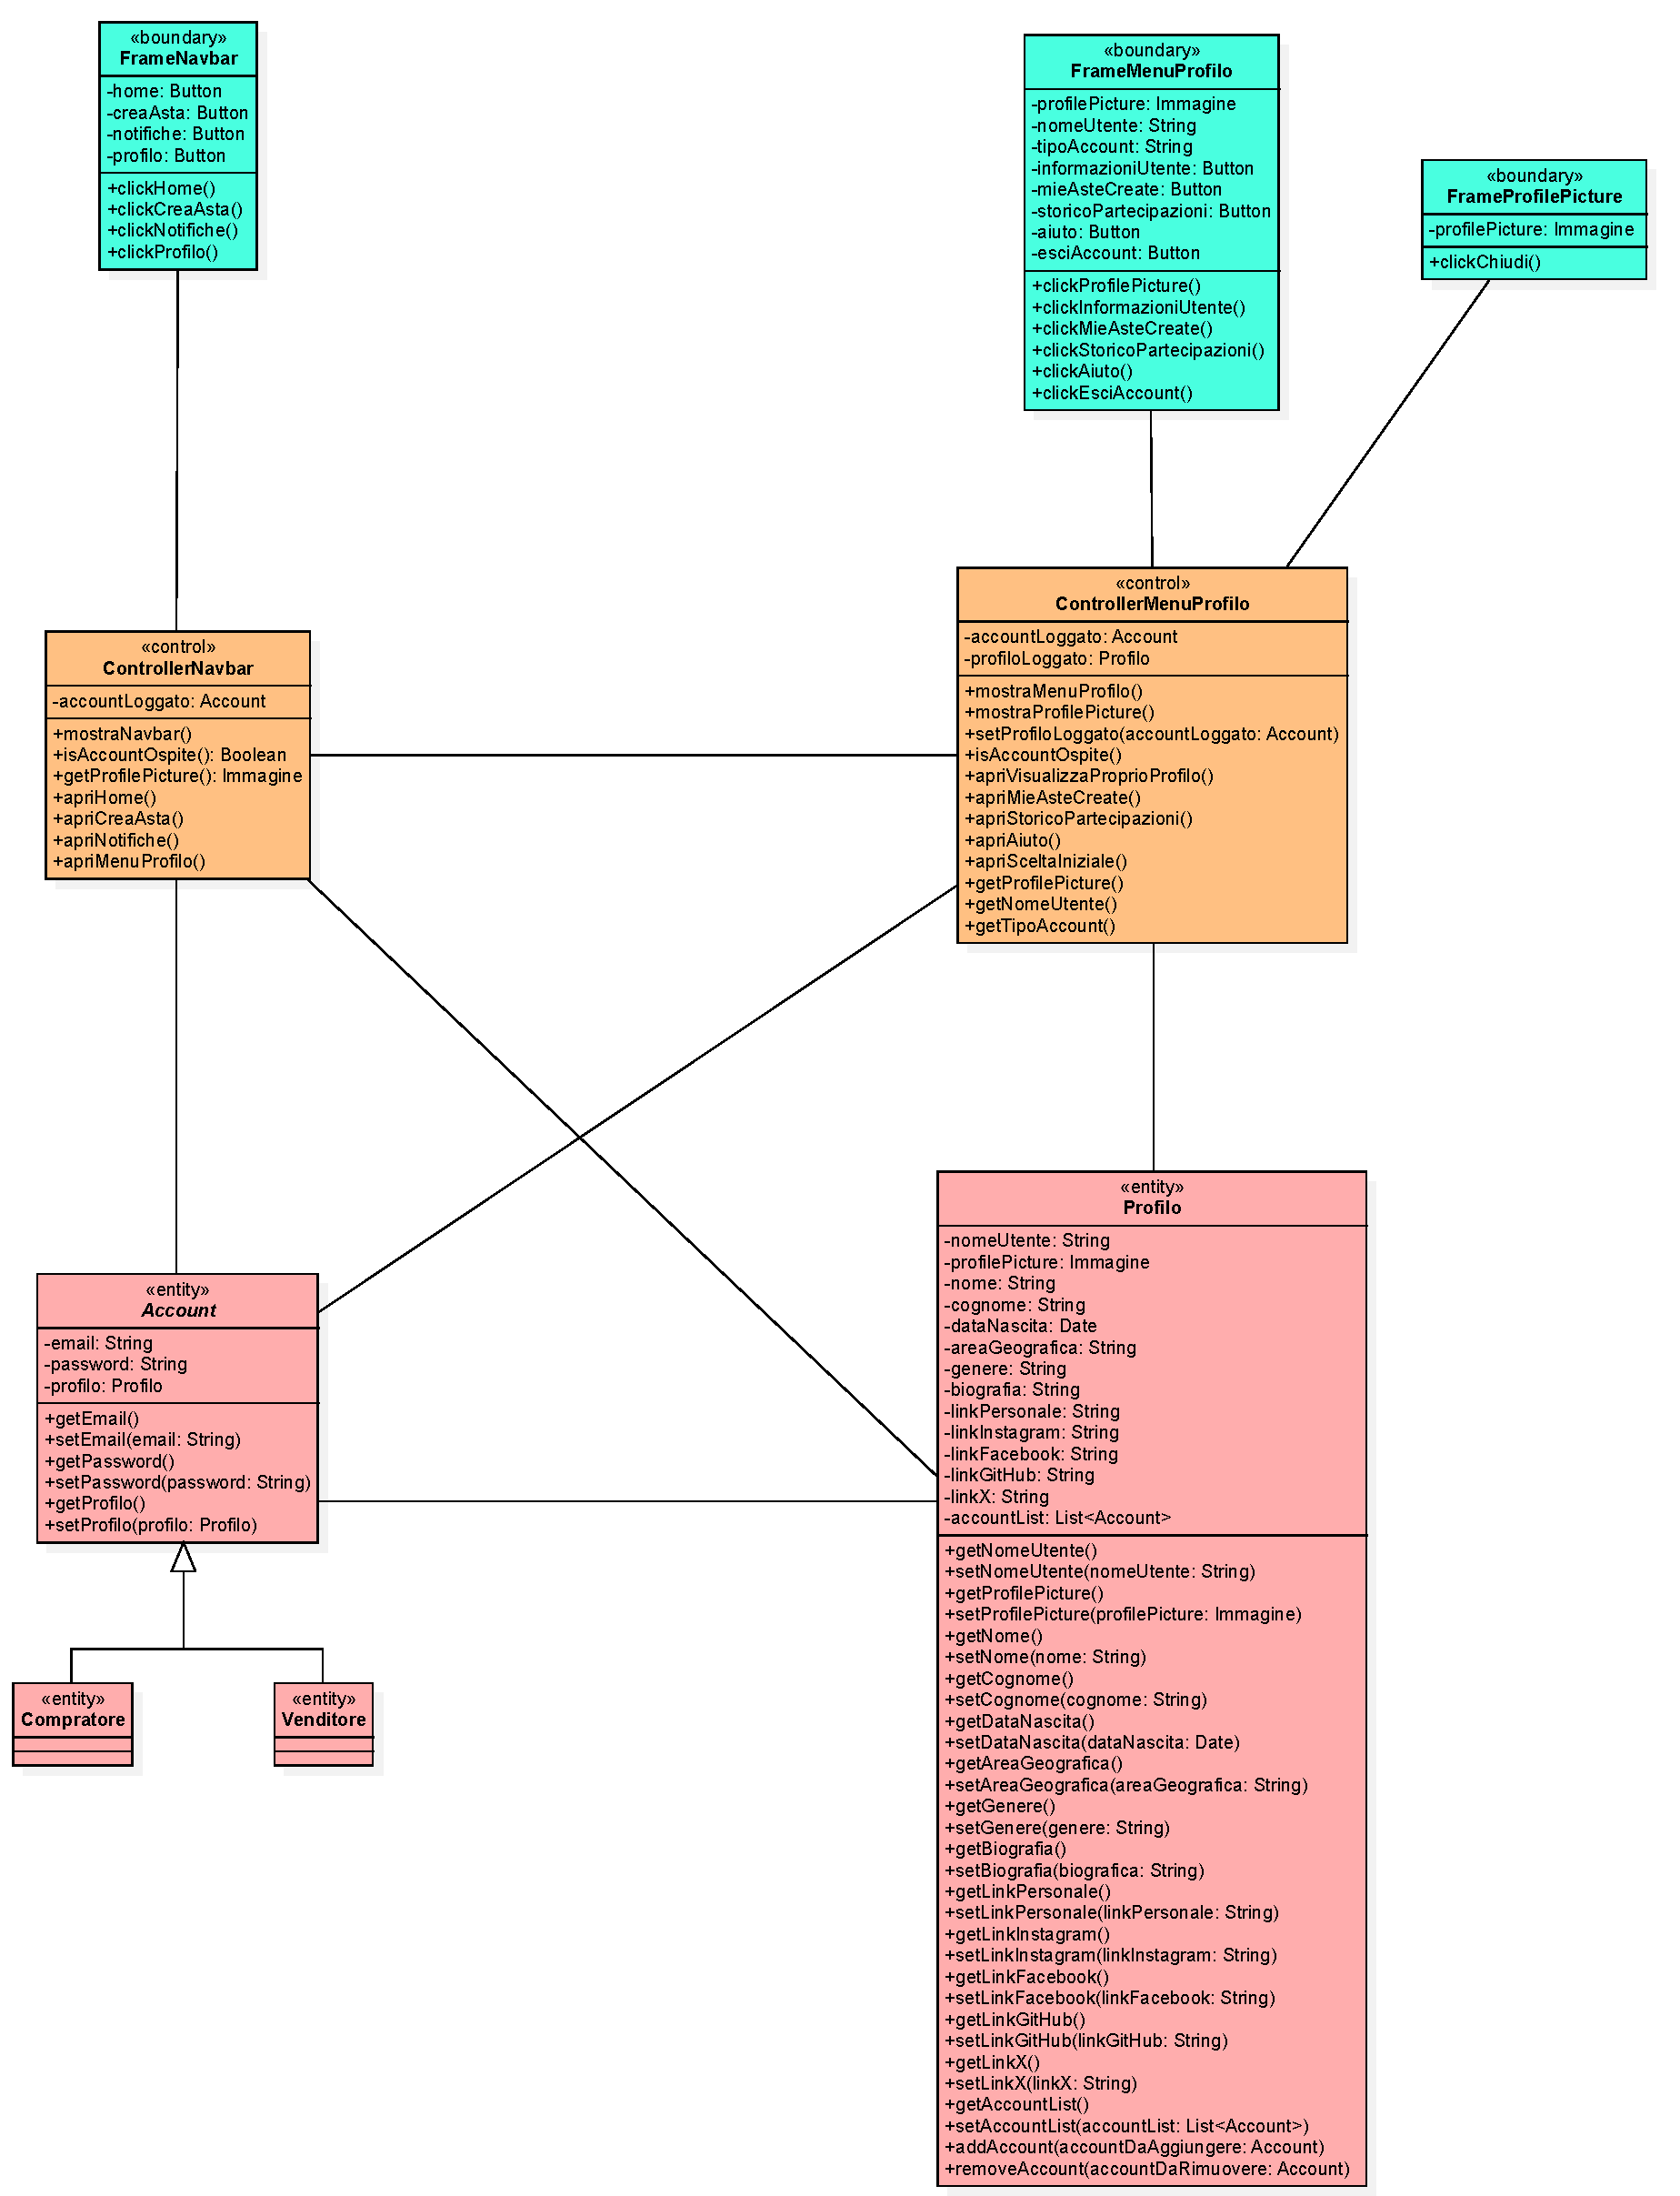
\includegraphics[width=1\linewidth]{Immagini/Diagrammi/Class Diagram/Utente che ha effettuato l'accesso/VisualizzaMenuProfilo.pdf}
                \caption{Visualizza menu profilo}
            \end{figure}
            
            \begin{figure}[htbp!]
                \centering
                    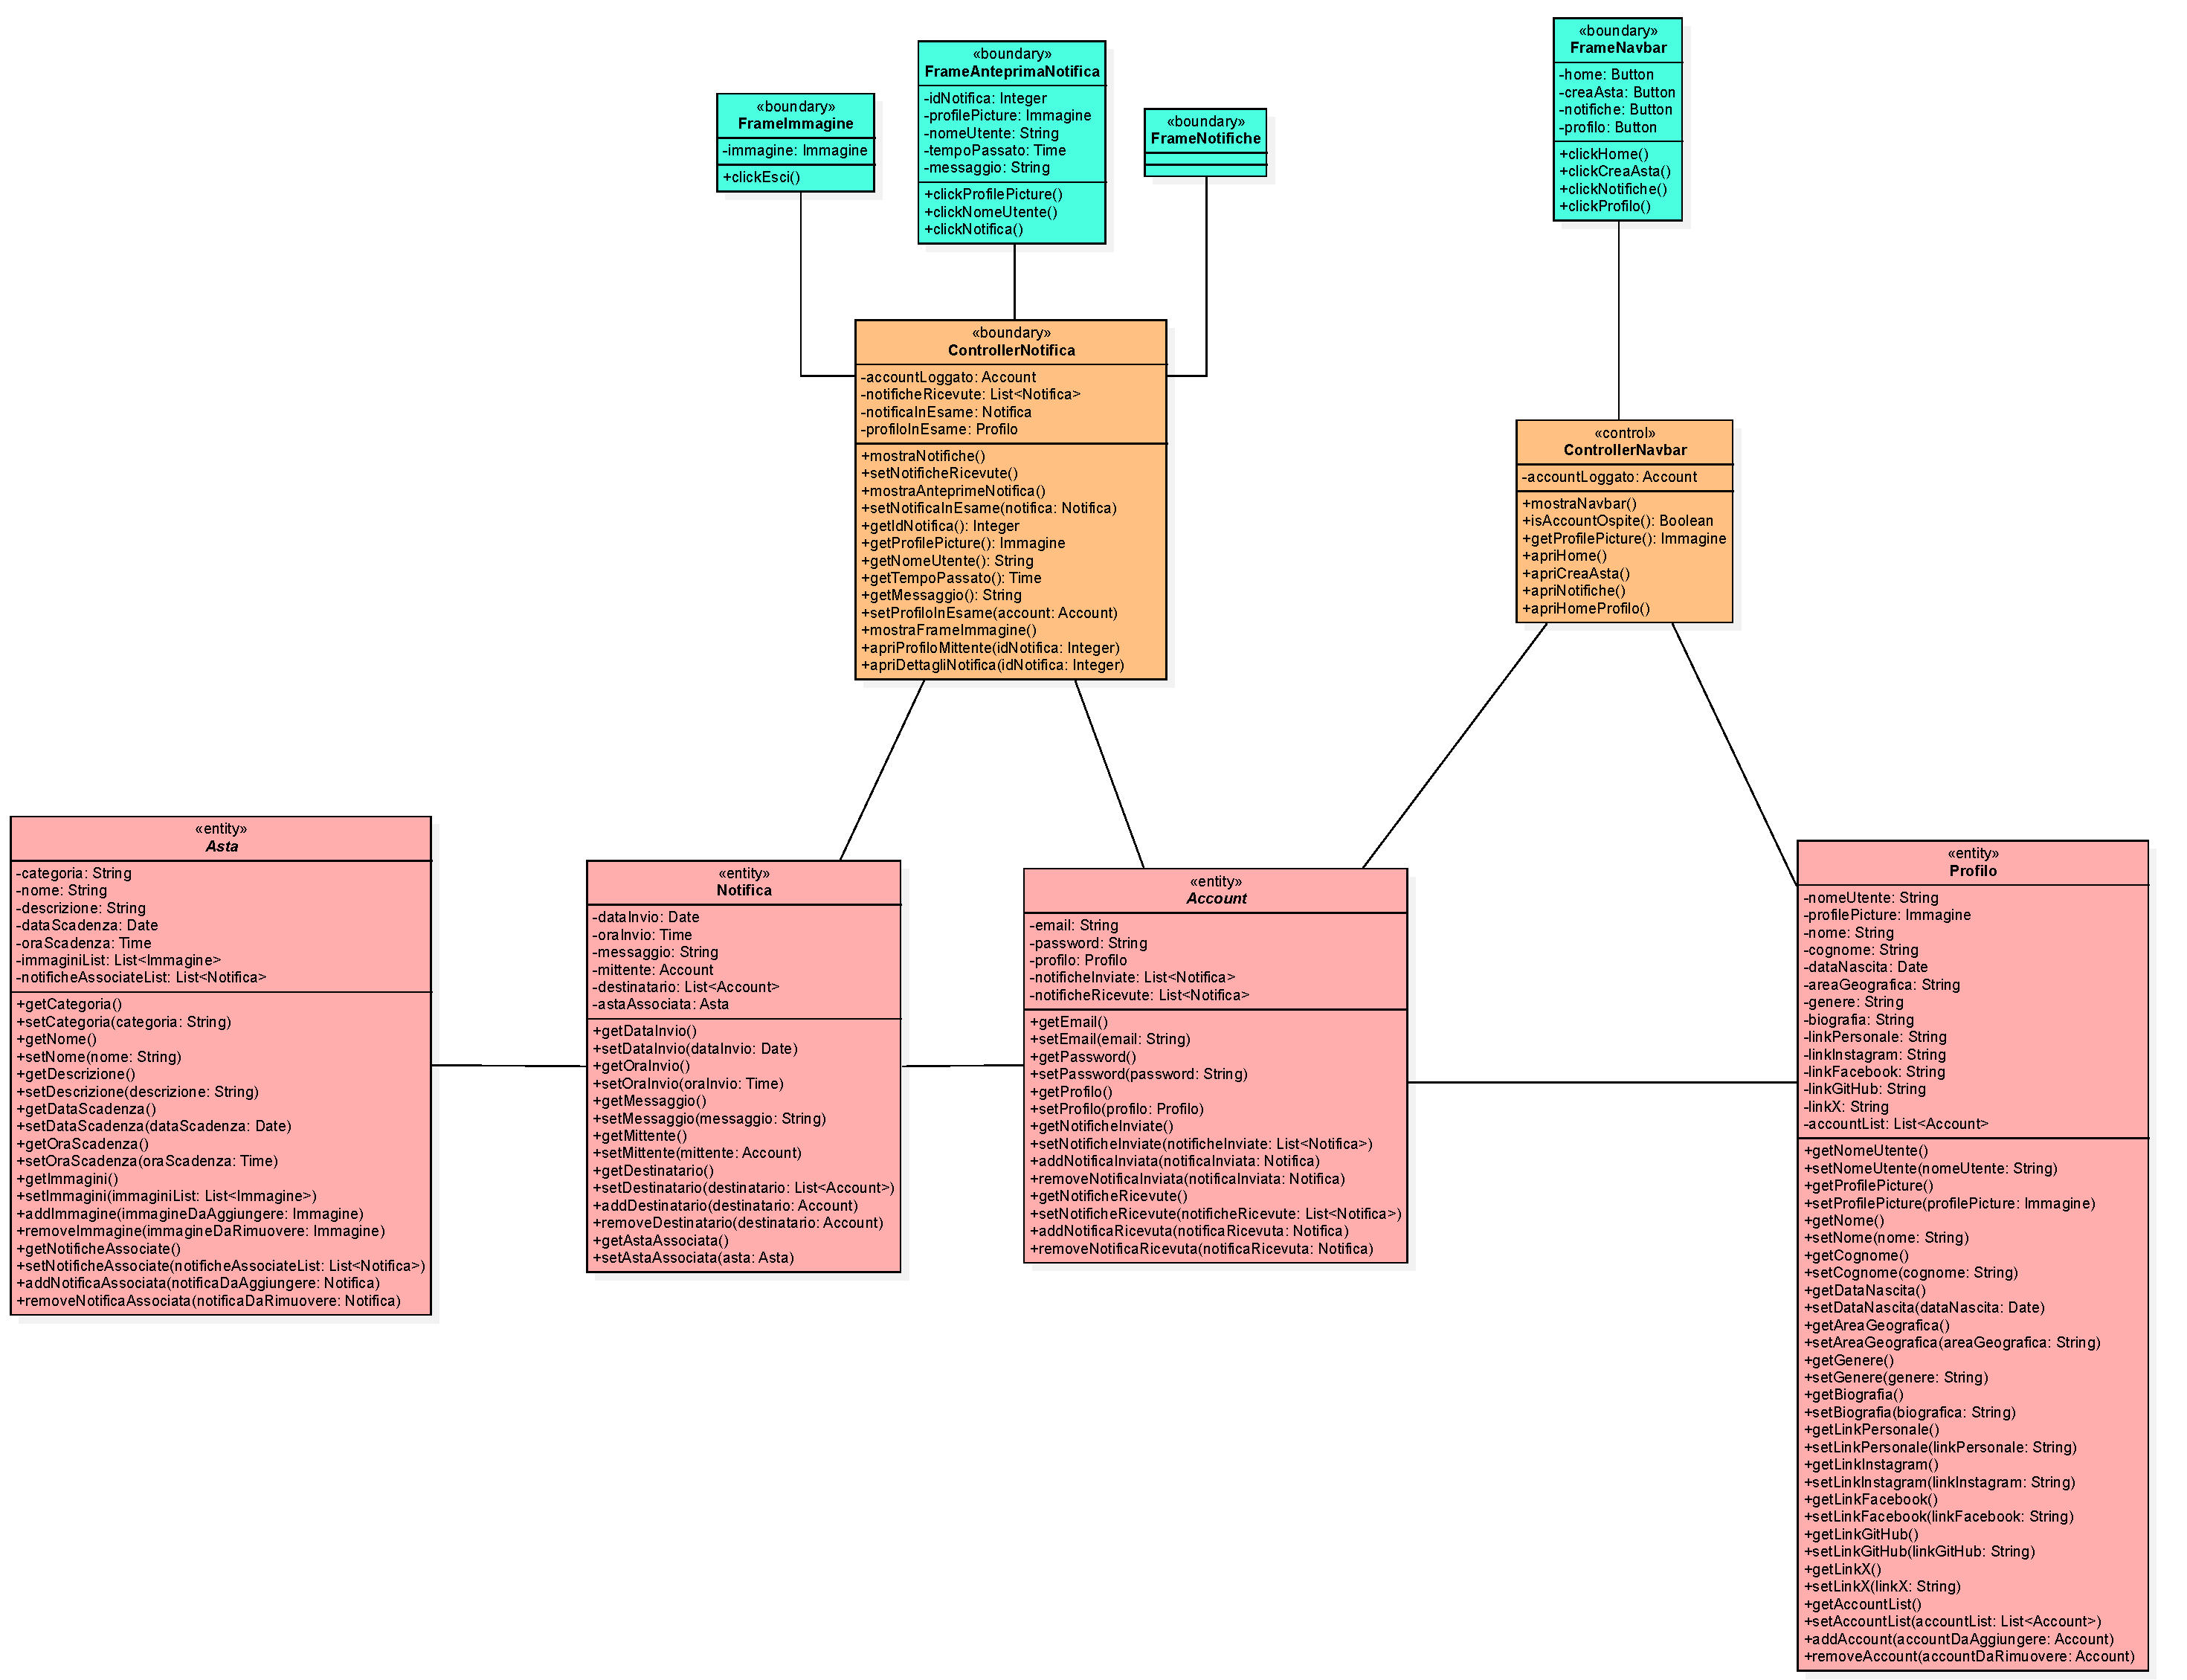
\includegraphics[width=1\linewidth]{Immagini/Diagrammi/Class Diagram/Utente che ha effettuato l'accesso/VisualizzaNotifiche.pdf}
                \caption{Visualizza notifiche}
            \end{figure}
            
            \begin{figure}[htbp!]
                \centering
                    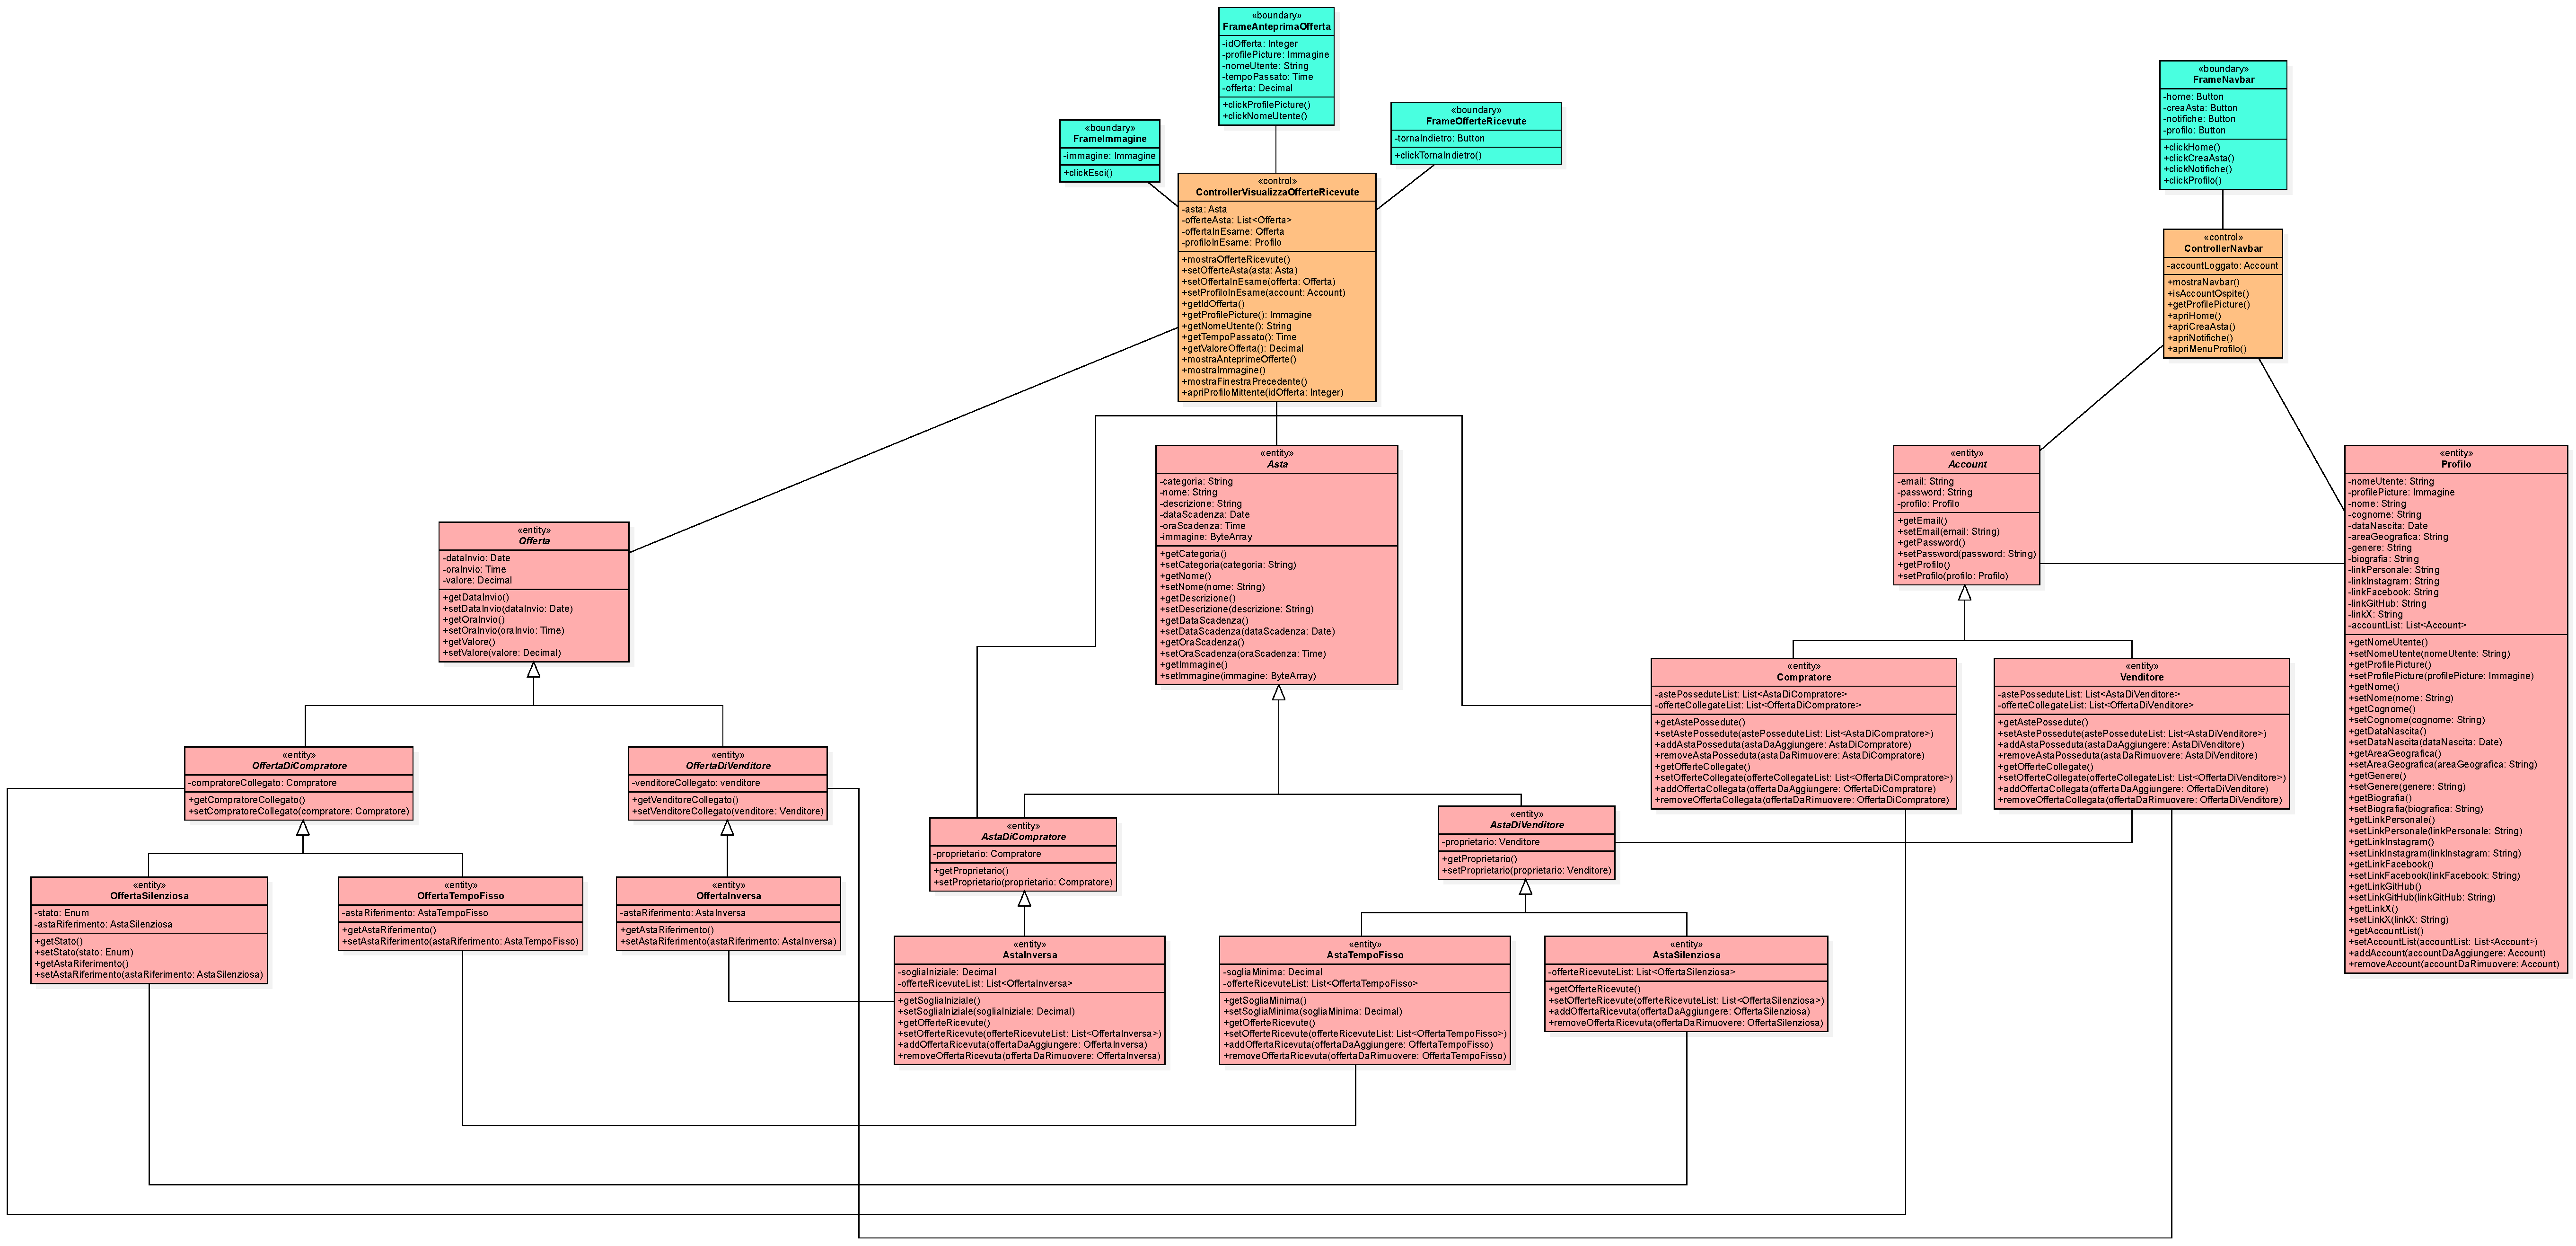
\includegraphics[width=1\linewidth]{Immagini/Diagrammi/Class Diagram/Utente che ha effettuato l'accesso/VisualizzaOfferteRicevute.pdf}
                \caption{Visualizza offerte ricevute}
            \end{figure}
            
            \begin{figure}[htbp!]
                \centering
                    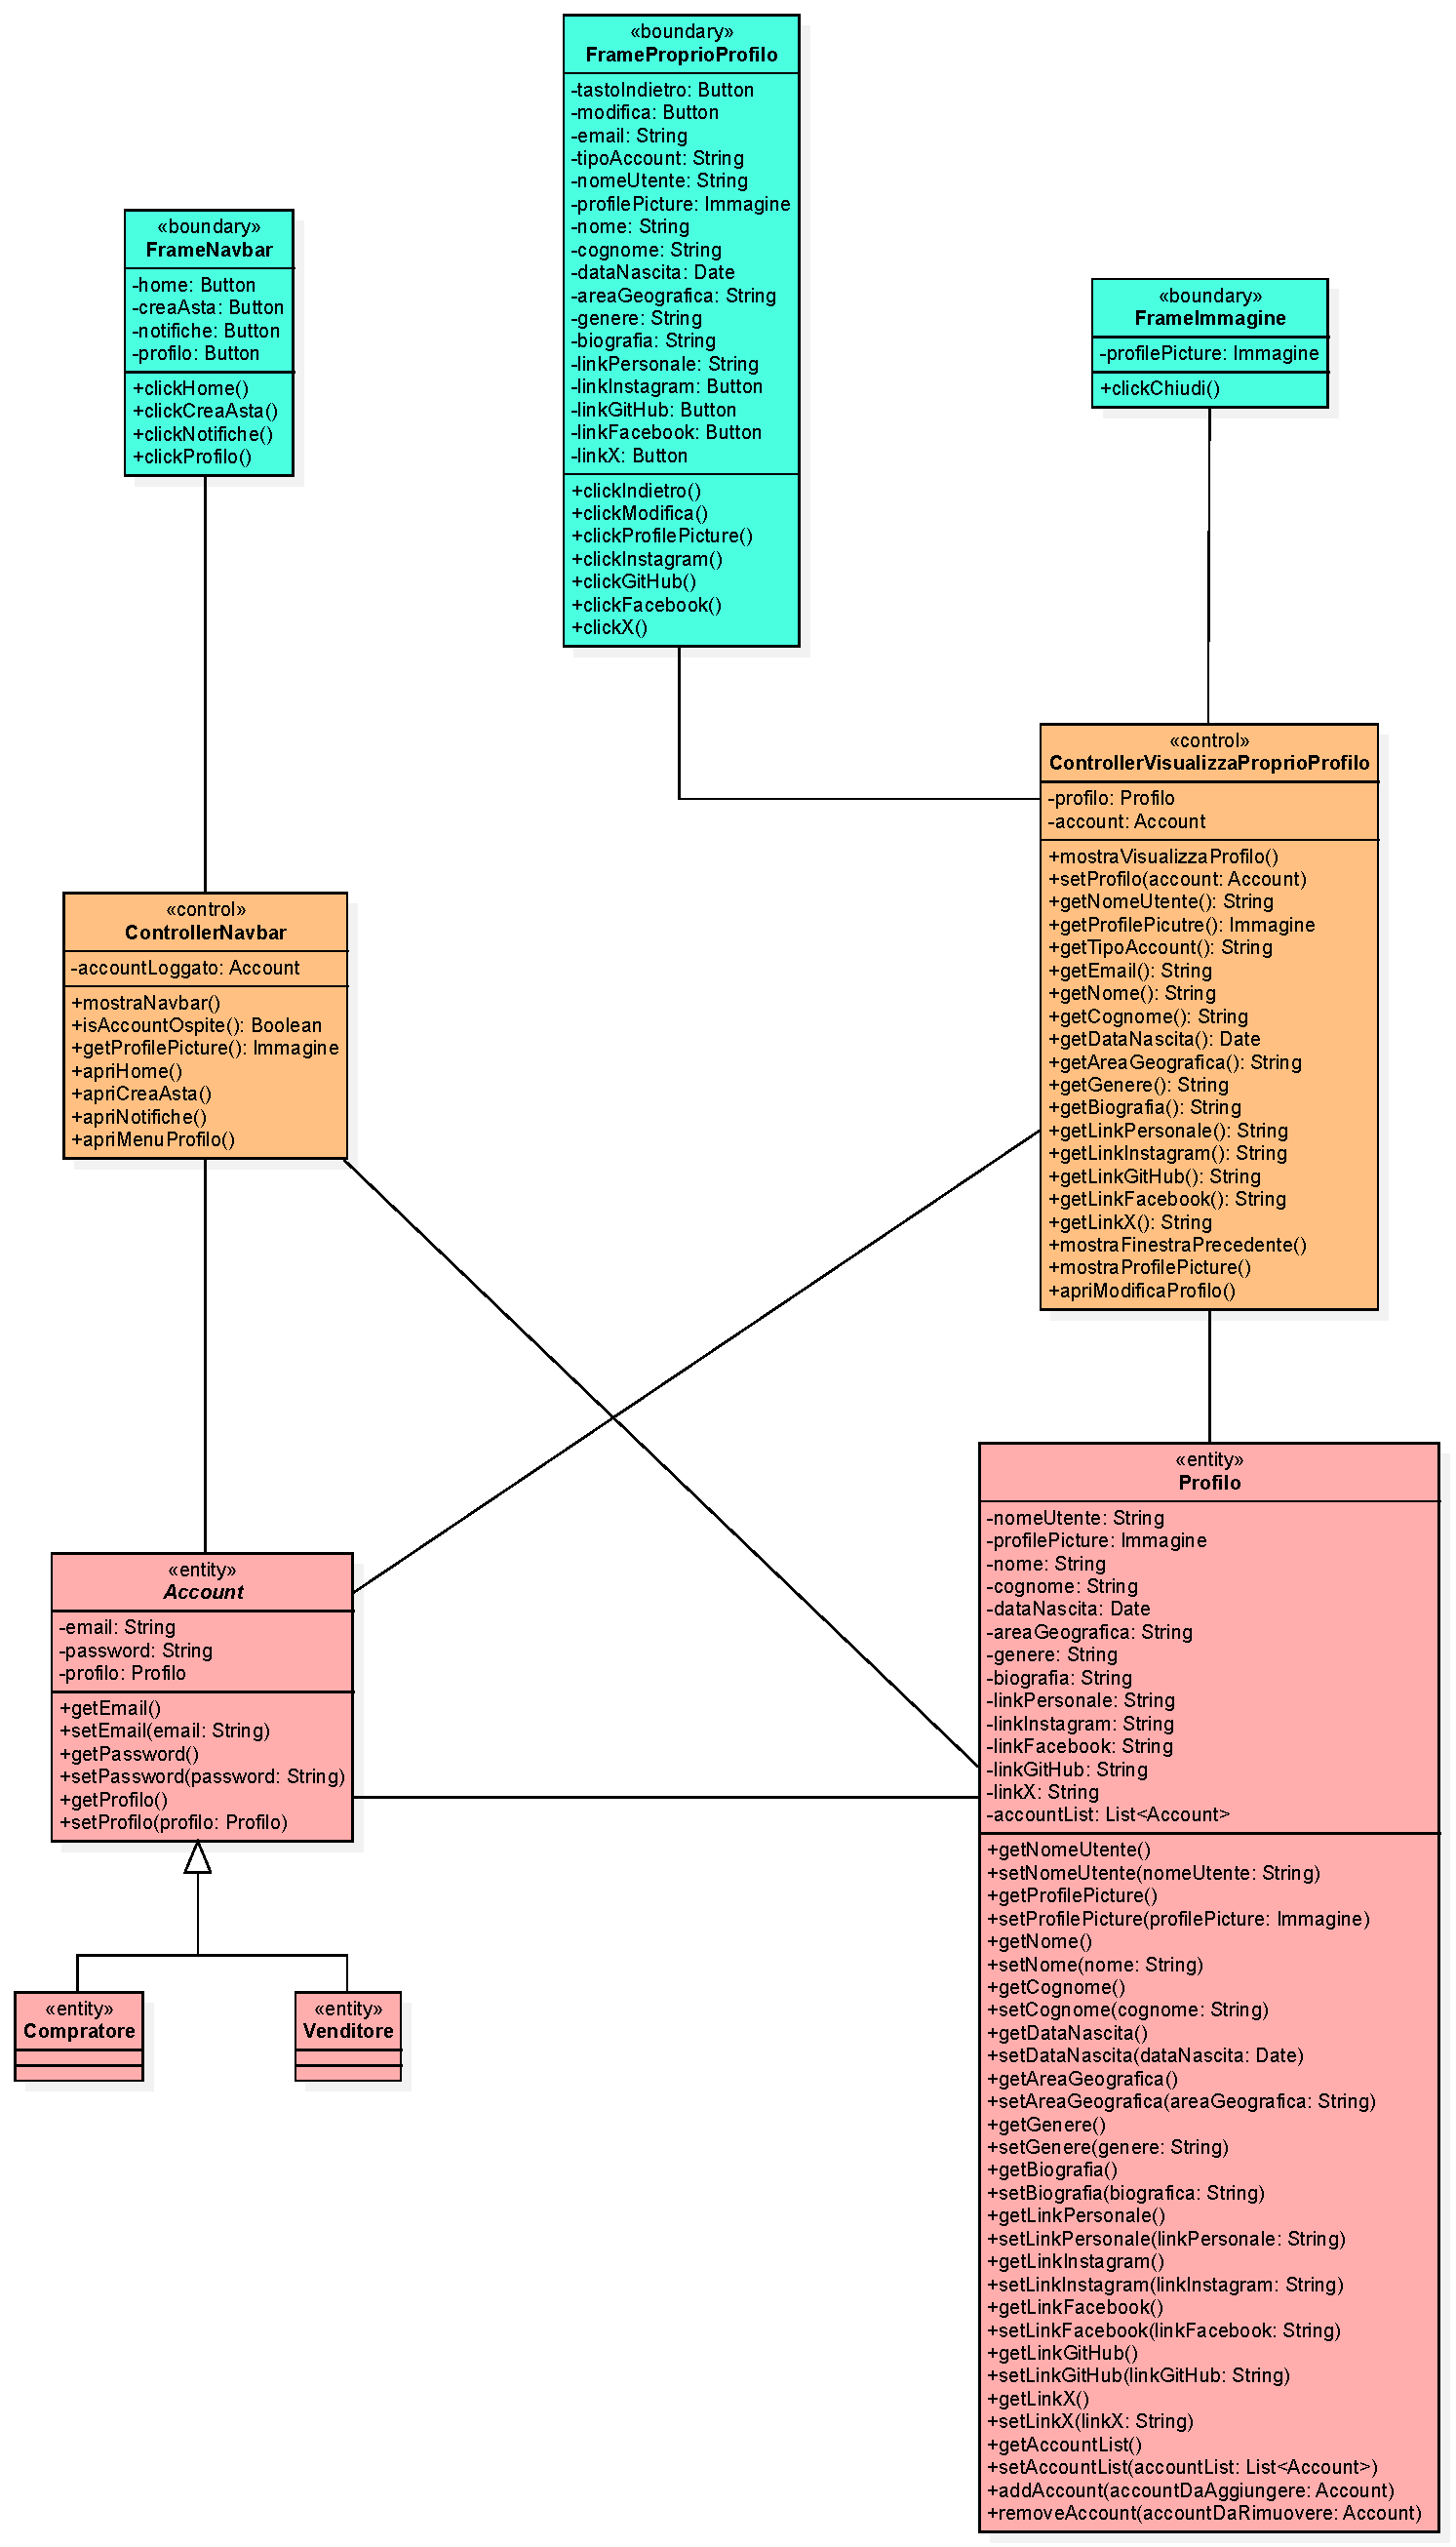
\includegraphics[width=0.75\linewidth]{Immagini/Diagrammi/Class Diagram/Utente che ha effettuato l'accesso/VisualizzaProprioProfilo.pdf}
                \caption{Visualizza profilo personale}
            \end{figure}
            
            \begin{figure}[htbp!]
                \centering
                    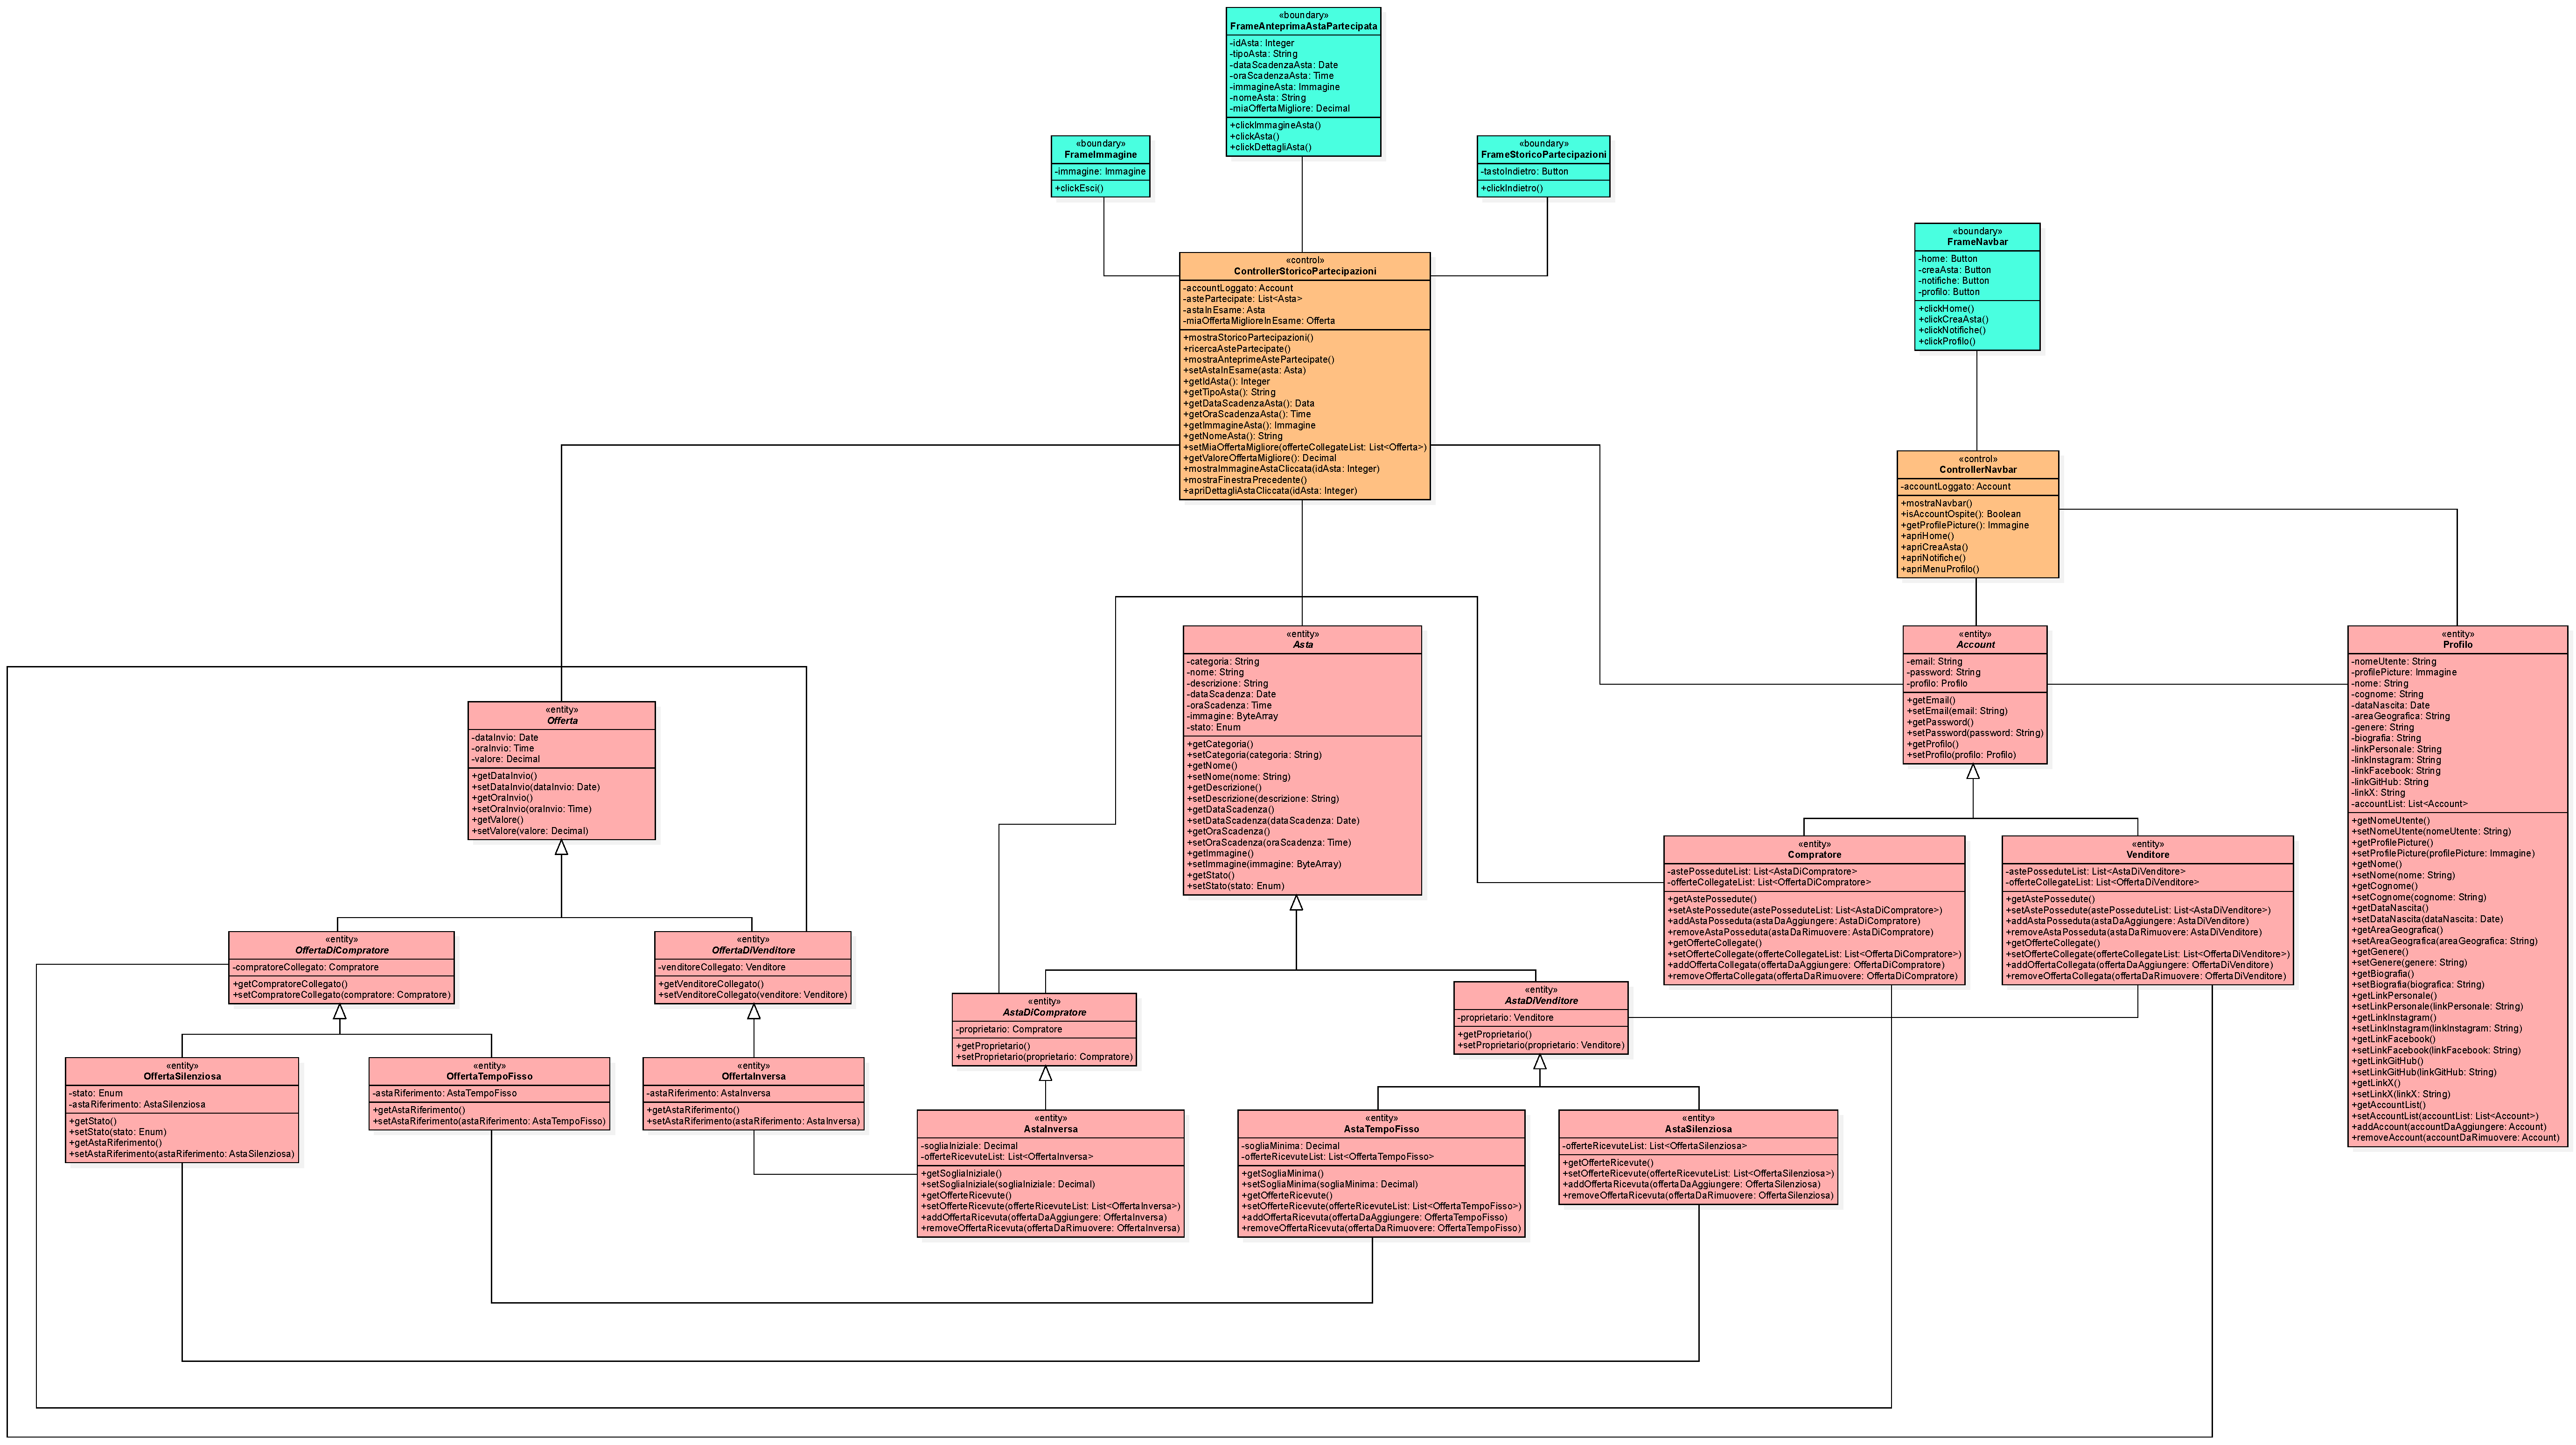
\includegraphics[width=1\linewidth]{Immagini/Diagrammi/Class Diagram/Utente che ha effettuato l'accesso/VisualizzaStoricoPartecipazioni.pdf}
                \caption{Visualizza aste partecipate}
            \end{figure}
            
            \begin{figure}[htbp!]
                \centering
                    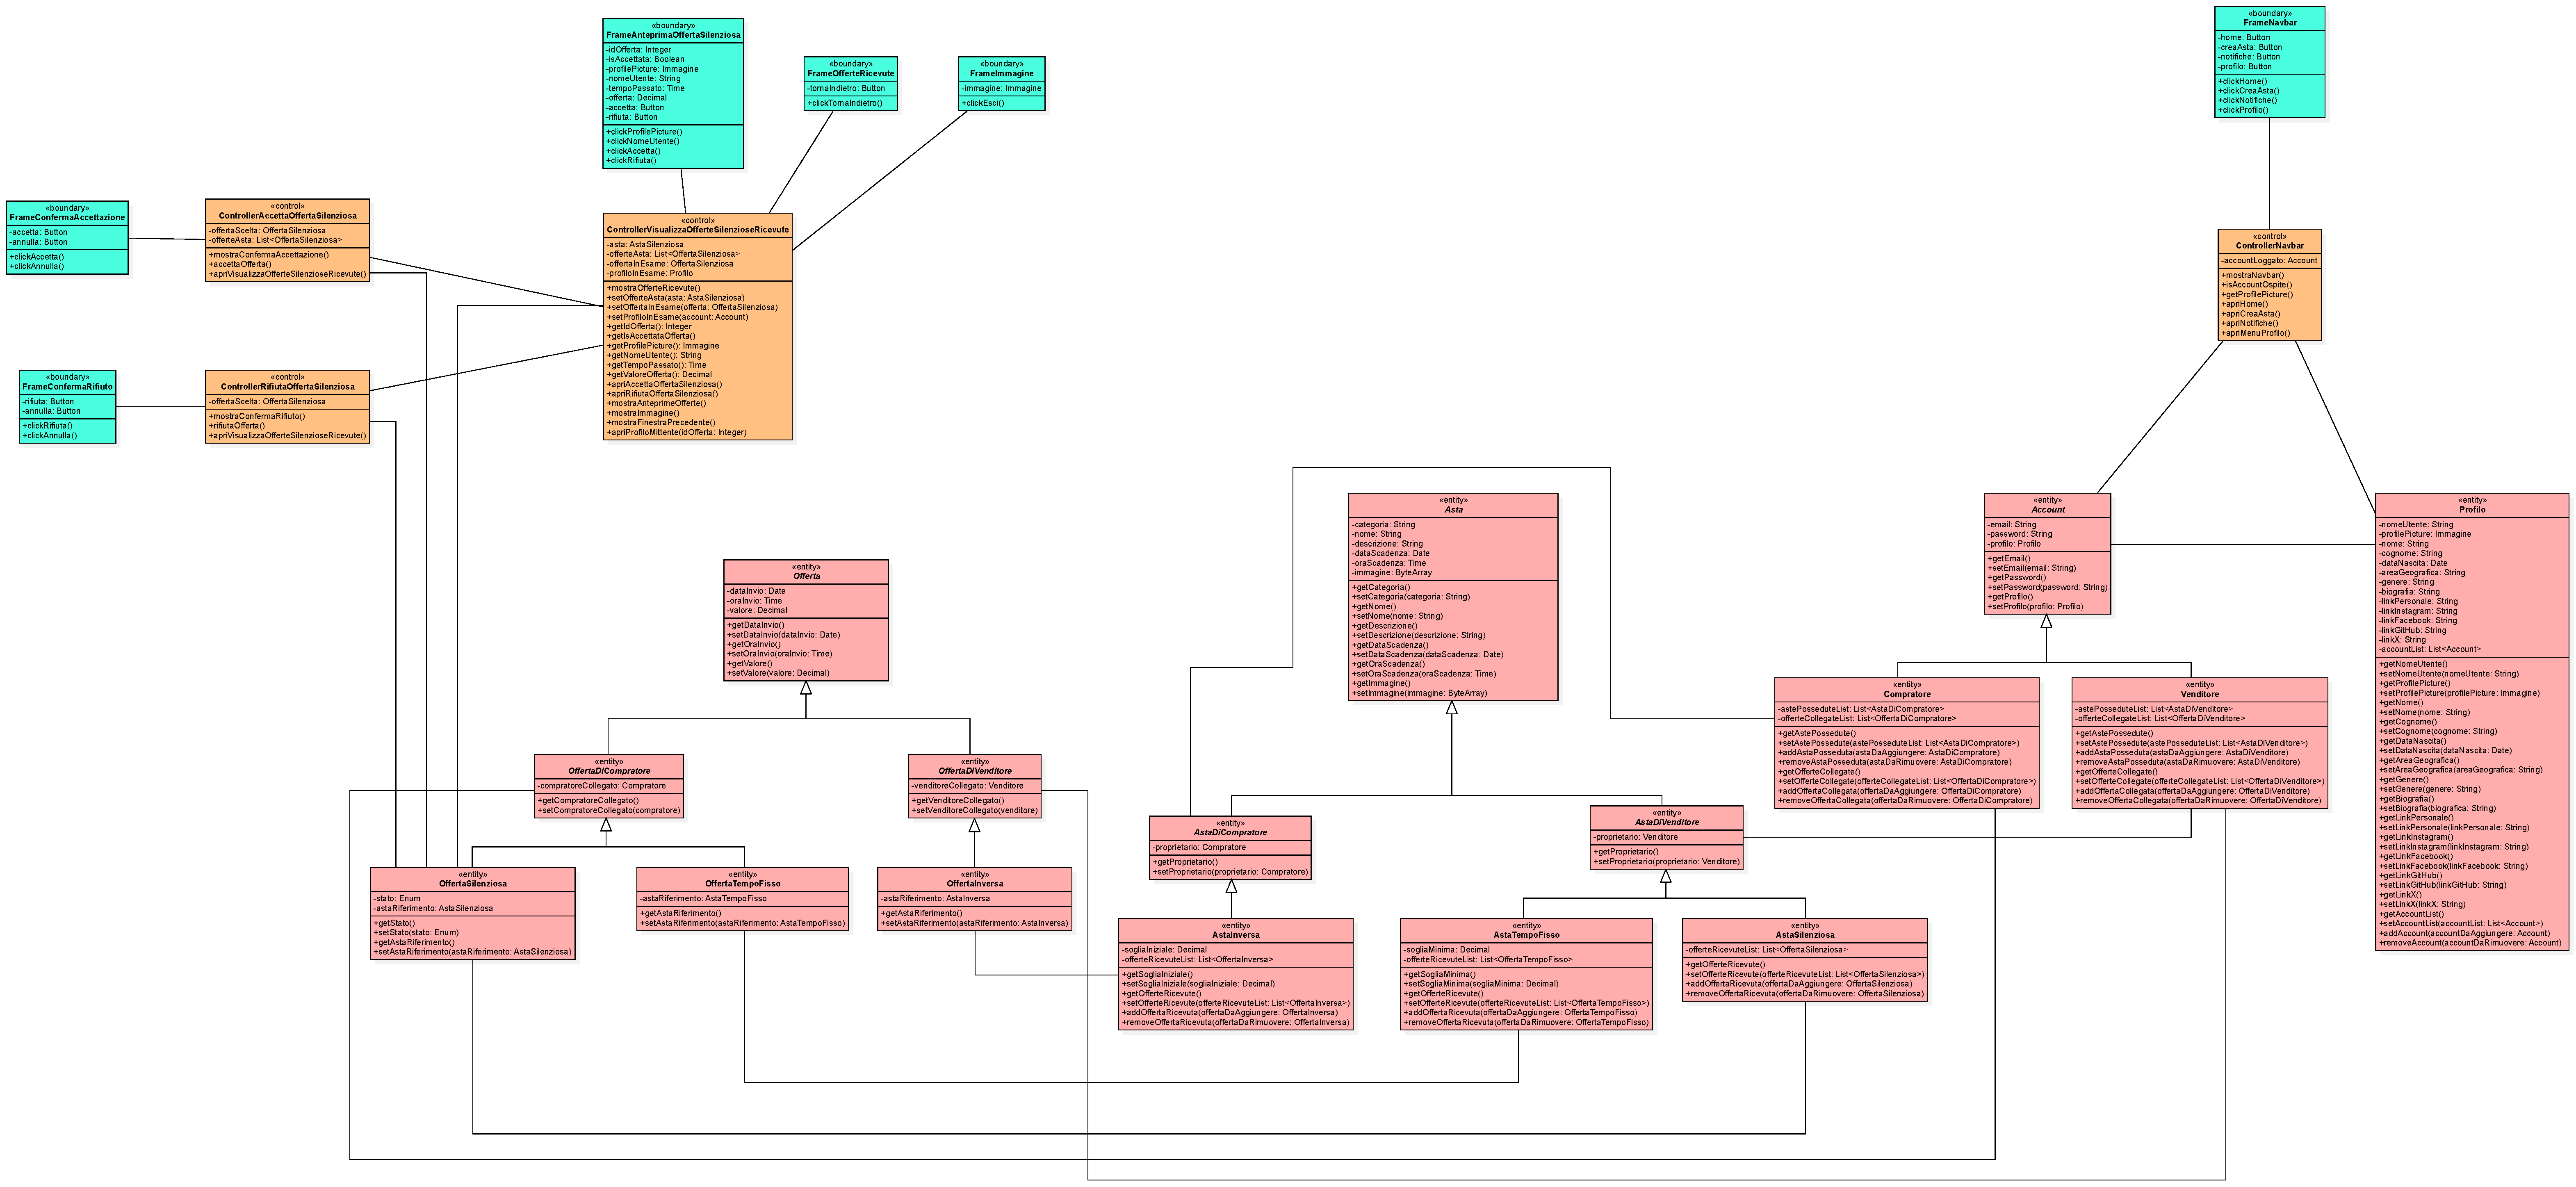
\includegraphics[width=1\linewidth]{Immagini/Diagrammi/Class Diagram/Venditore e compratore/AccettaRifiutaOffertaSilenziosa.pdf}
                \caption{Accetta o rifiuta un'offerta per un'asta silenziosa}
            \end{figure}
            
            \begin{figure}[htbp!]
                \centering
                    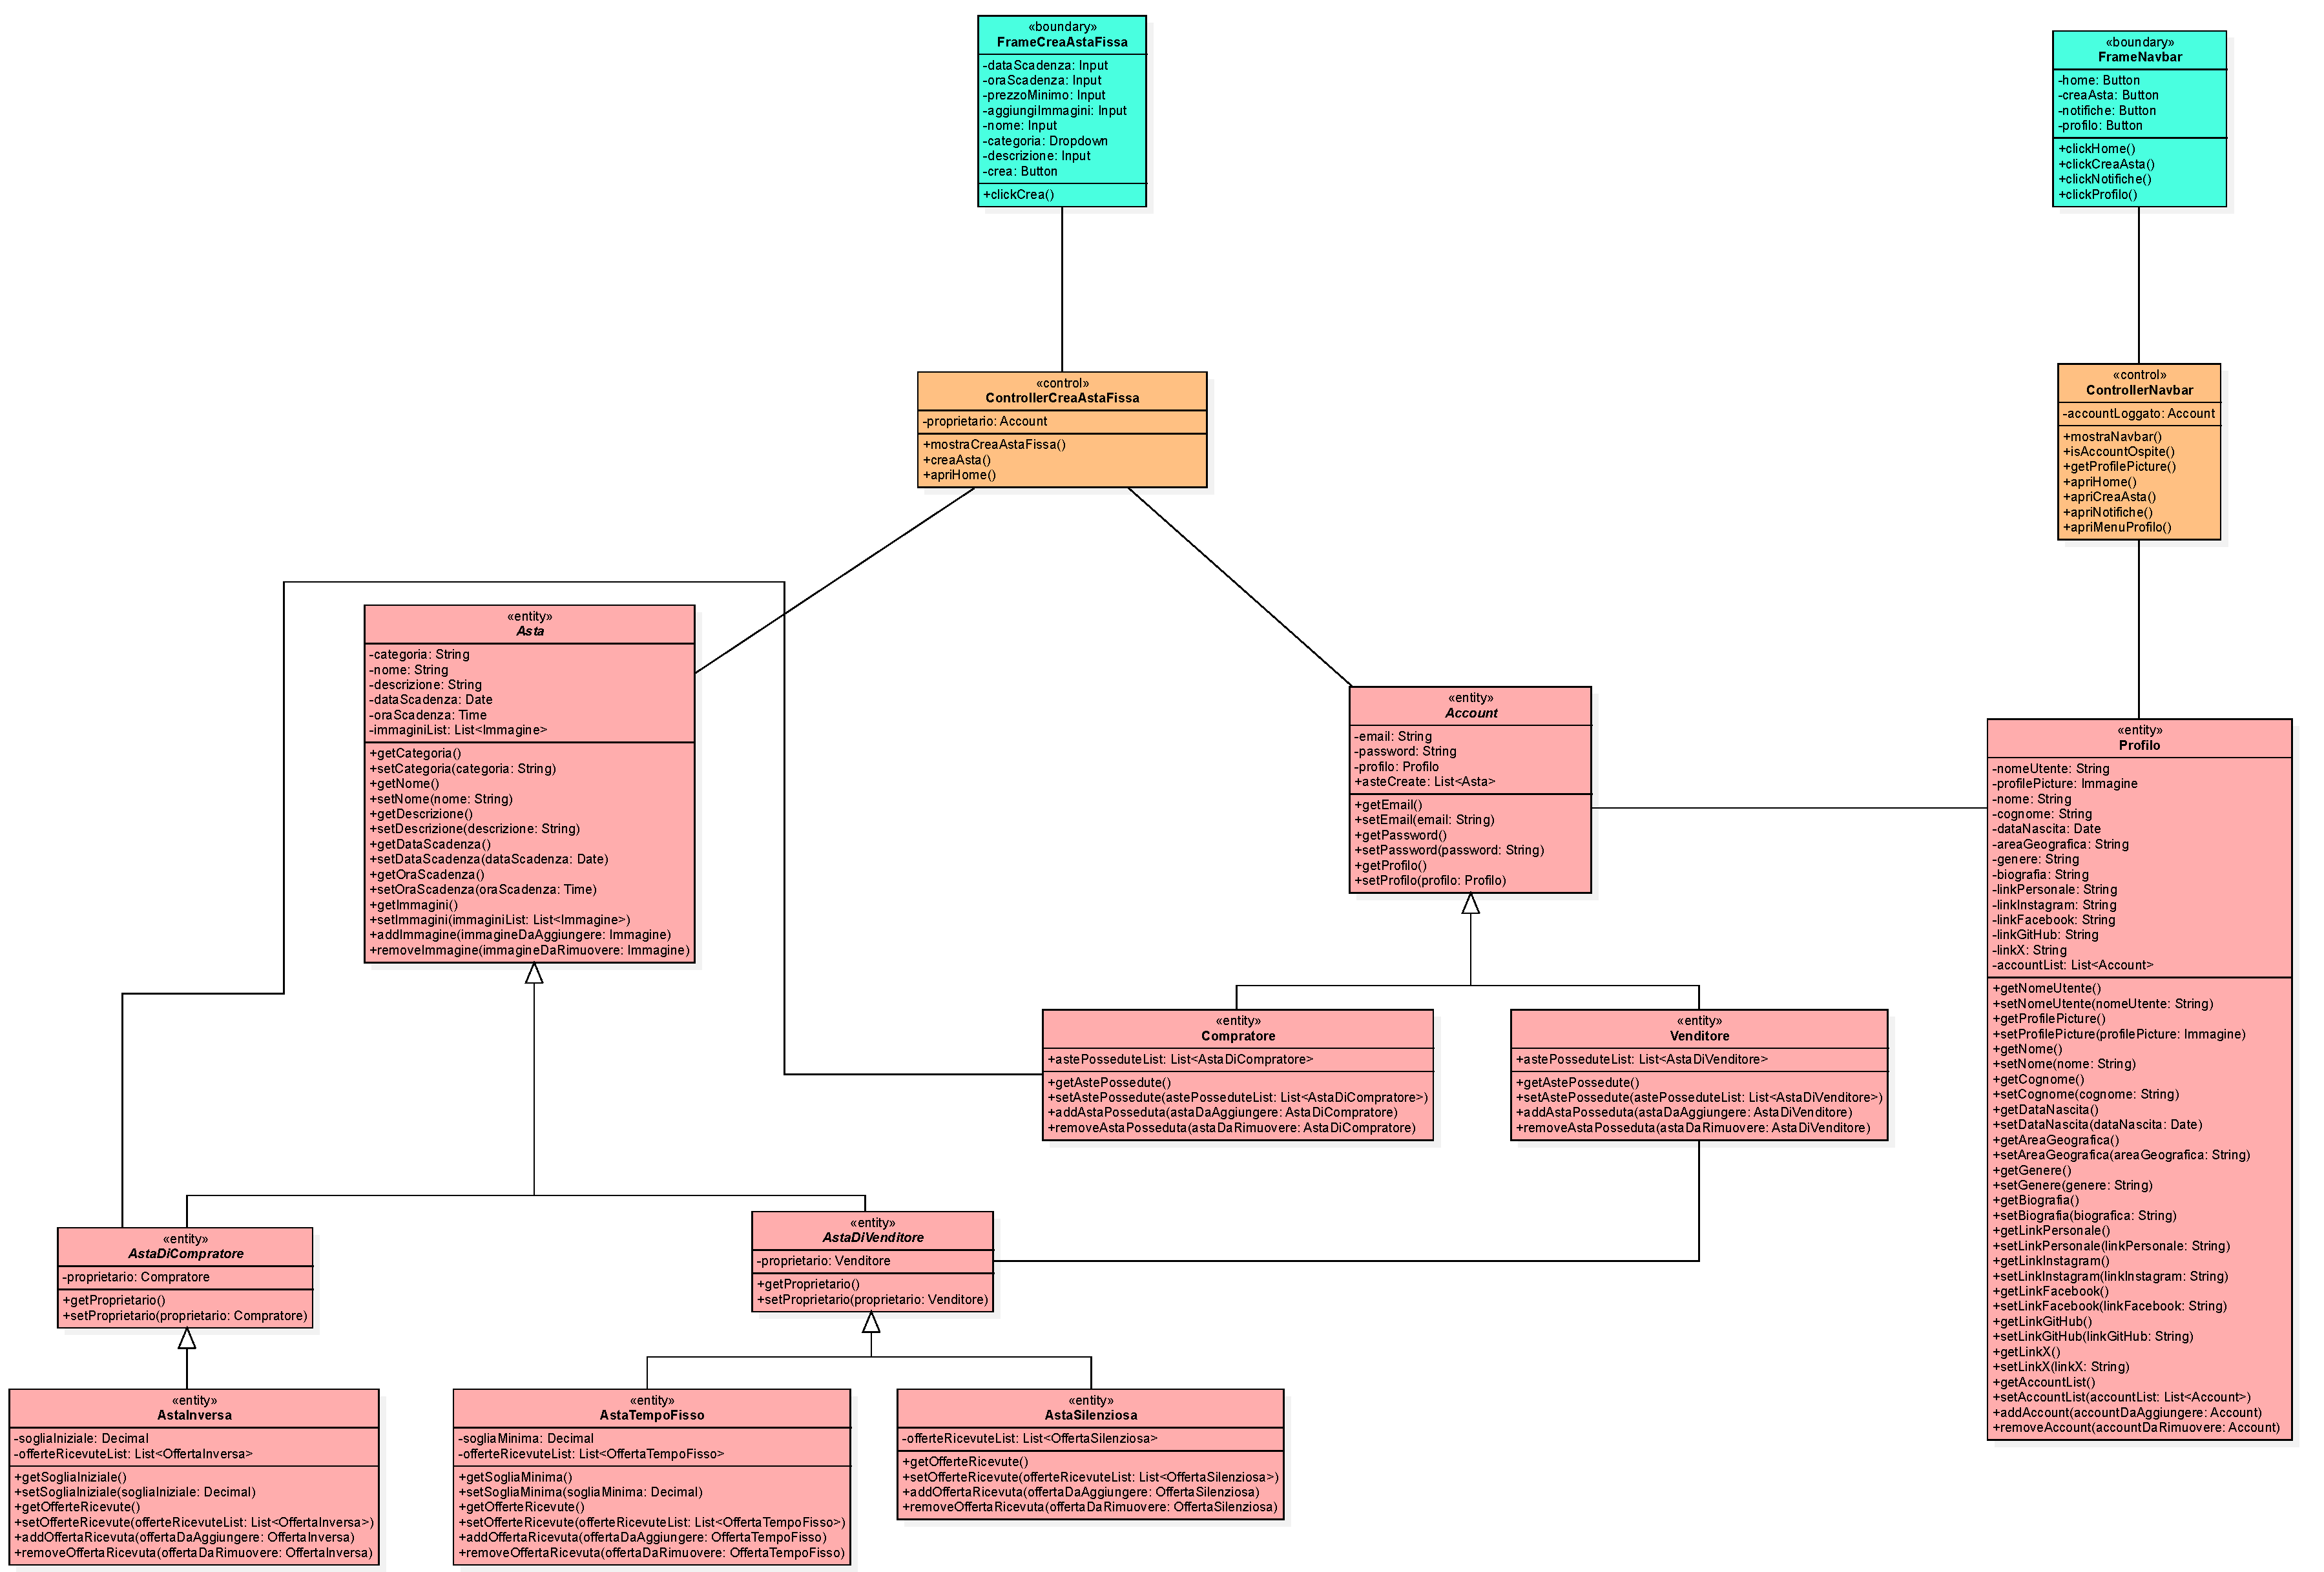
\includegraphics[width=1\linewidth]{Immagini/Diagrammi/Class Diagram/Venditore e compratore/CreaAstaFissa.pdf}
                \caption{Crea un'asta a tempo fisso}
            \end{figure}
            
            \begin{figure}[htbp!]
                \centering
                    \includegraphics[width=1\linewidth]{Immagini/Diagrammi/Class Diagram/Venditore e compratore/CreaAstaInversa.pdf}
                \caption{Crea un'asta inversa}
            \end{figure}
            
            \begin{figure}[htbp!]
                \centering
                    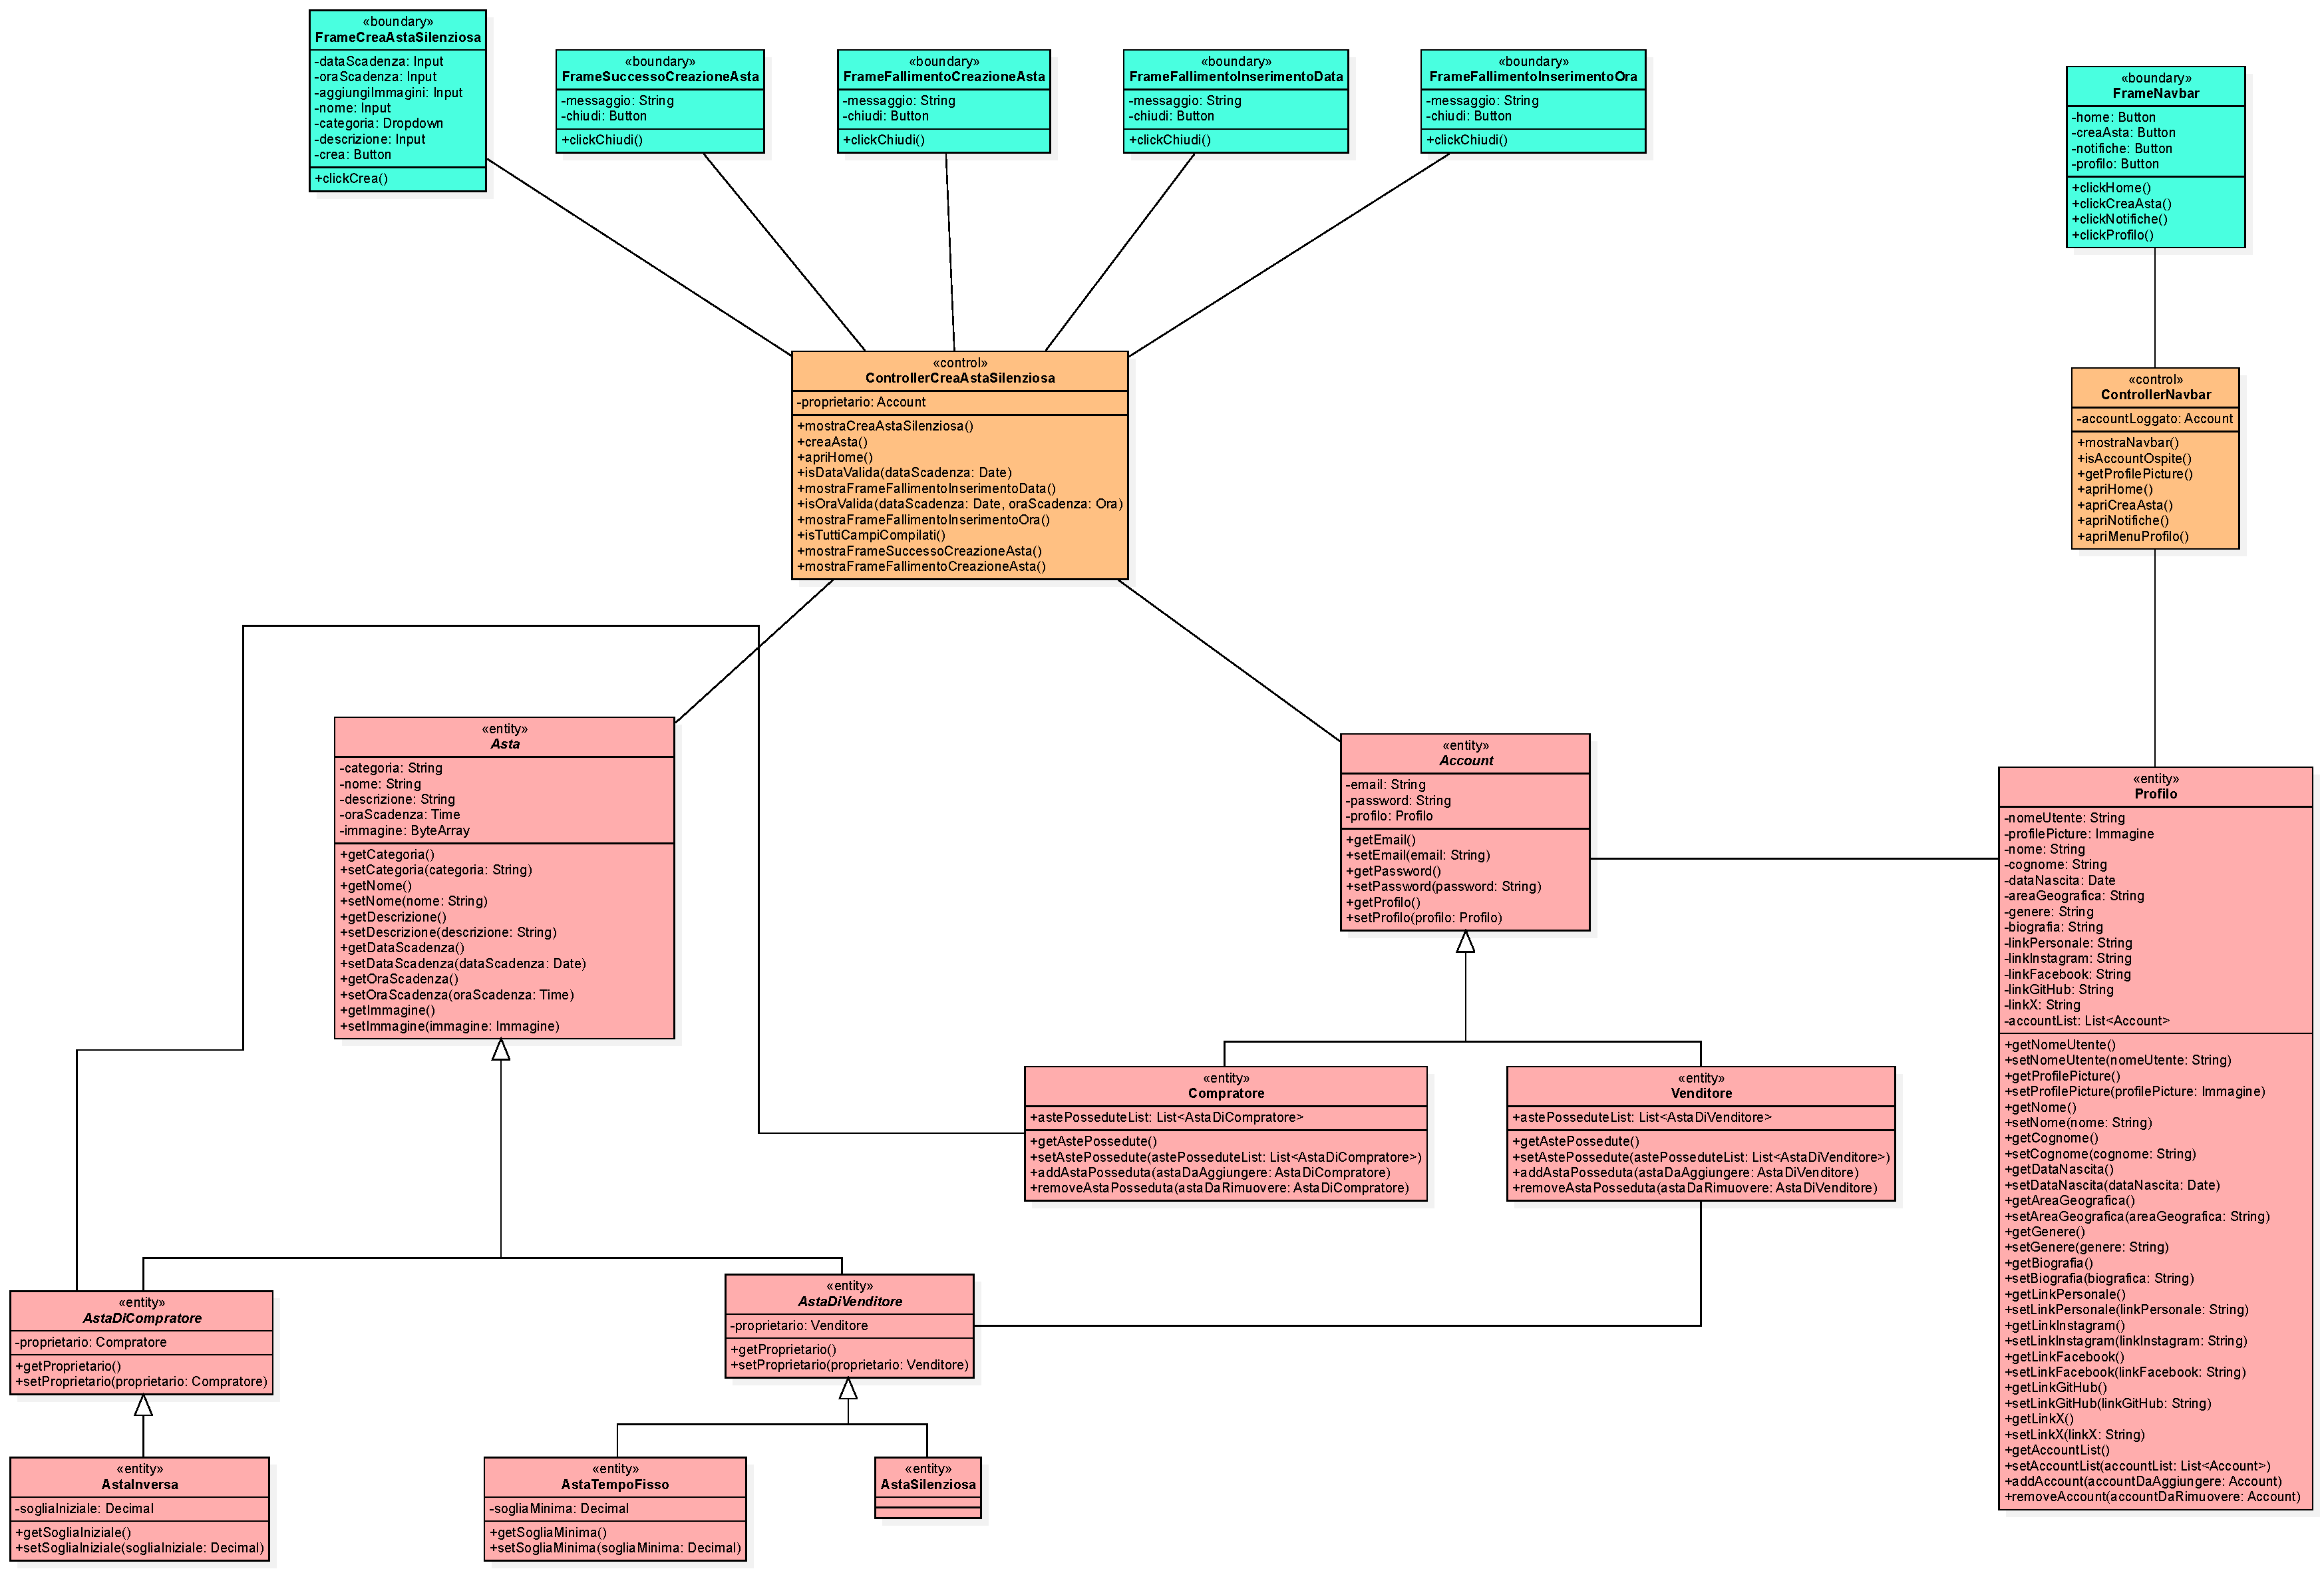
\includegraphics[width=1\linewidth]{Immagini/Diagrammi/Class Diagram/Venditore e compratore/CreaAstaSilenziosa.pdf}
                \caption{Crea un'asta silenziosa}
            \end{figure}
            
            \begin{figure}[htbp!]
                \centering
                    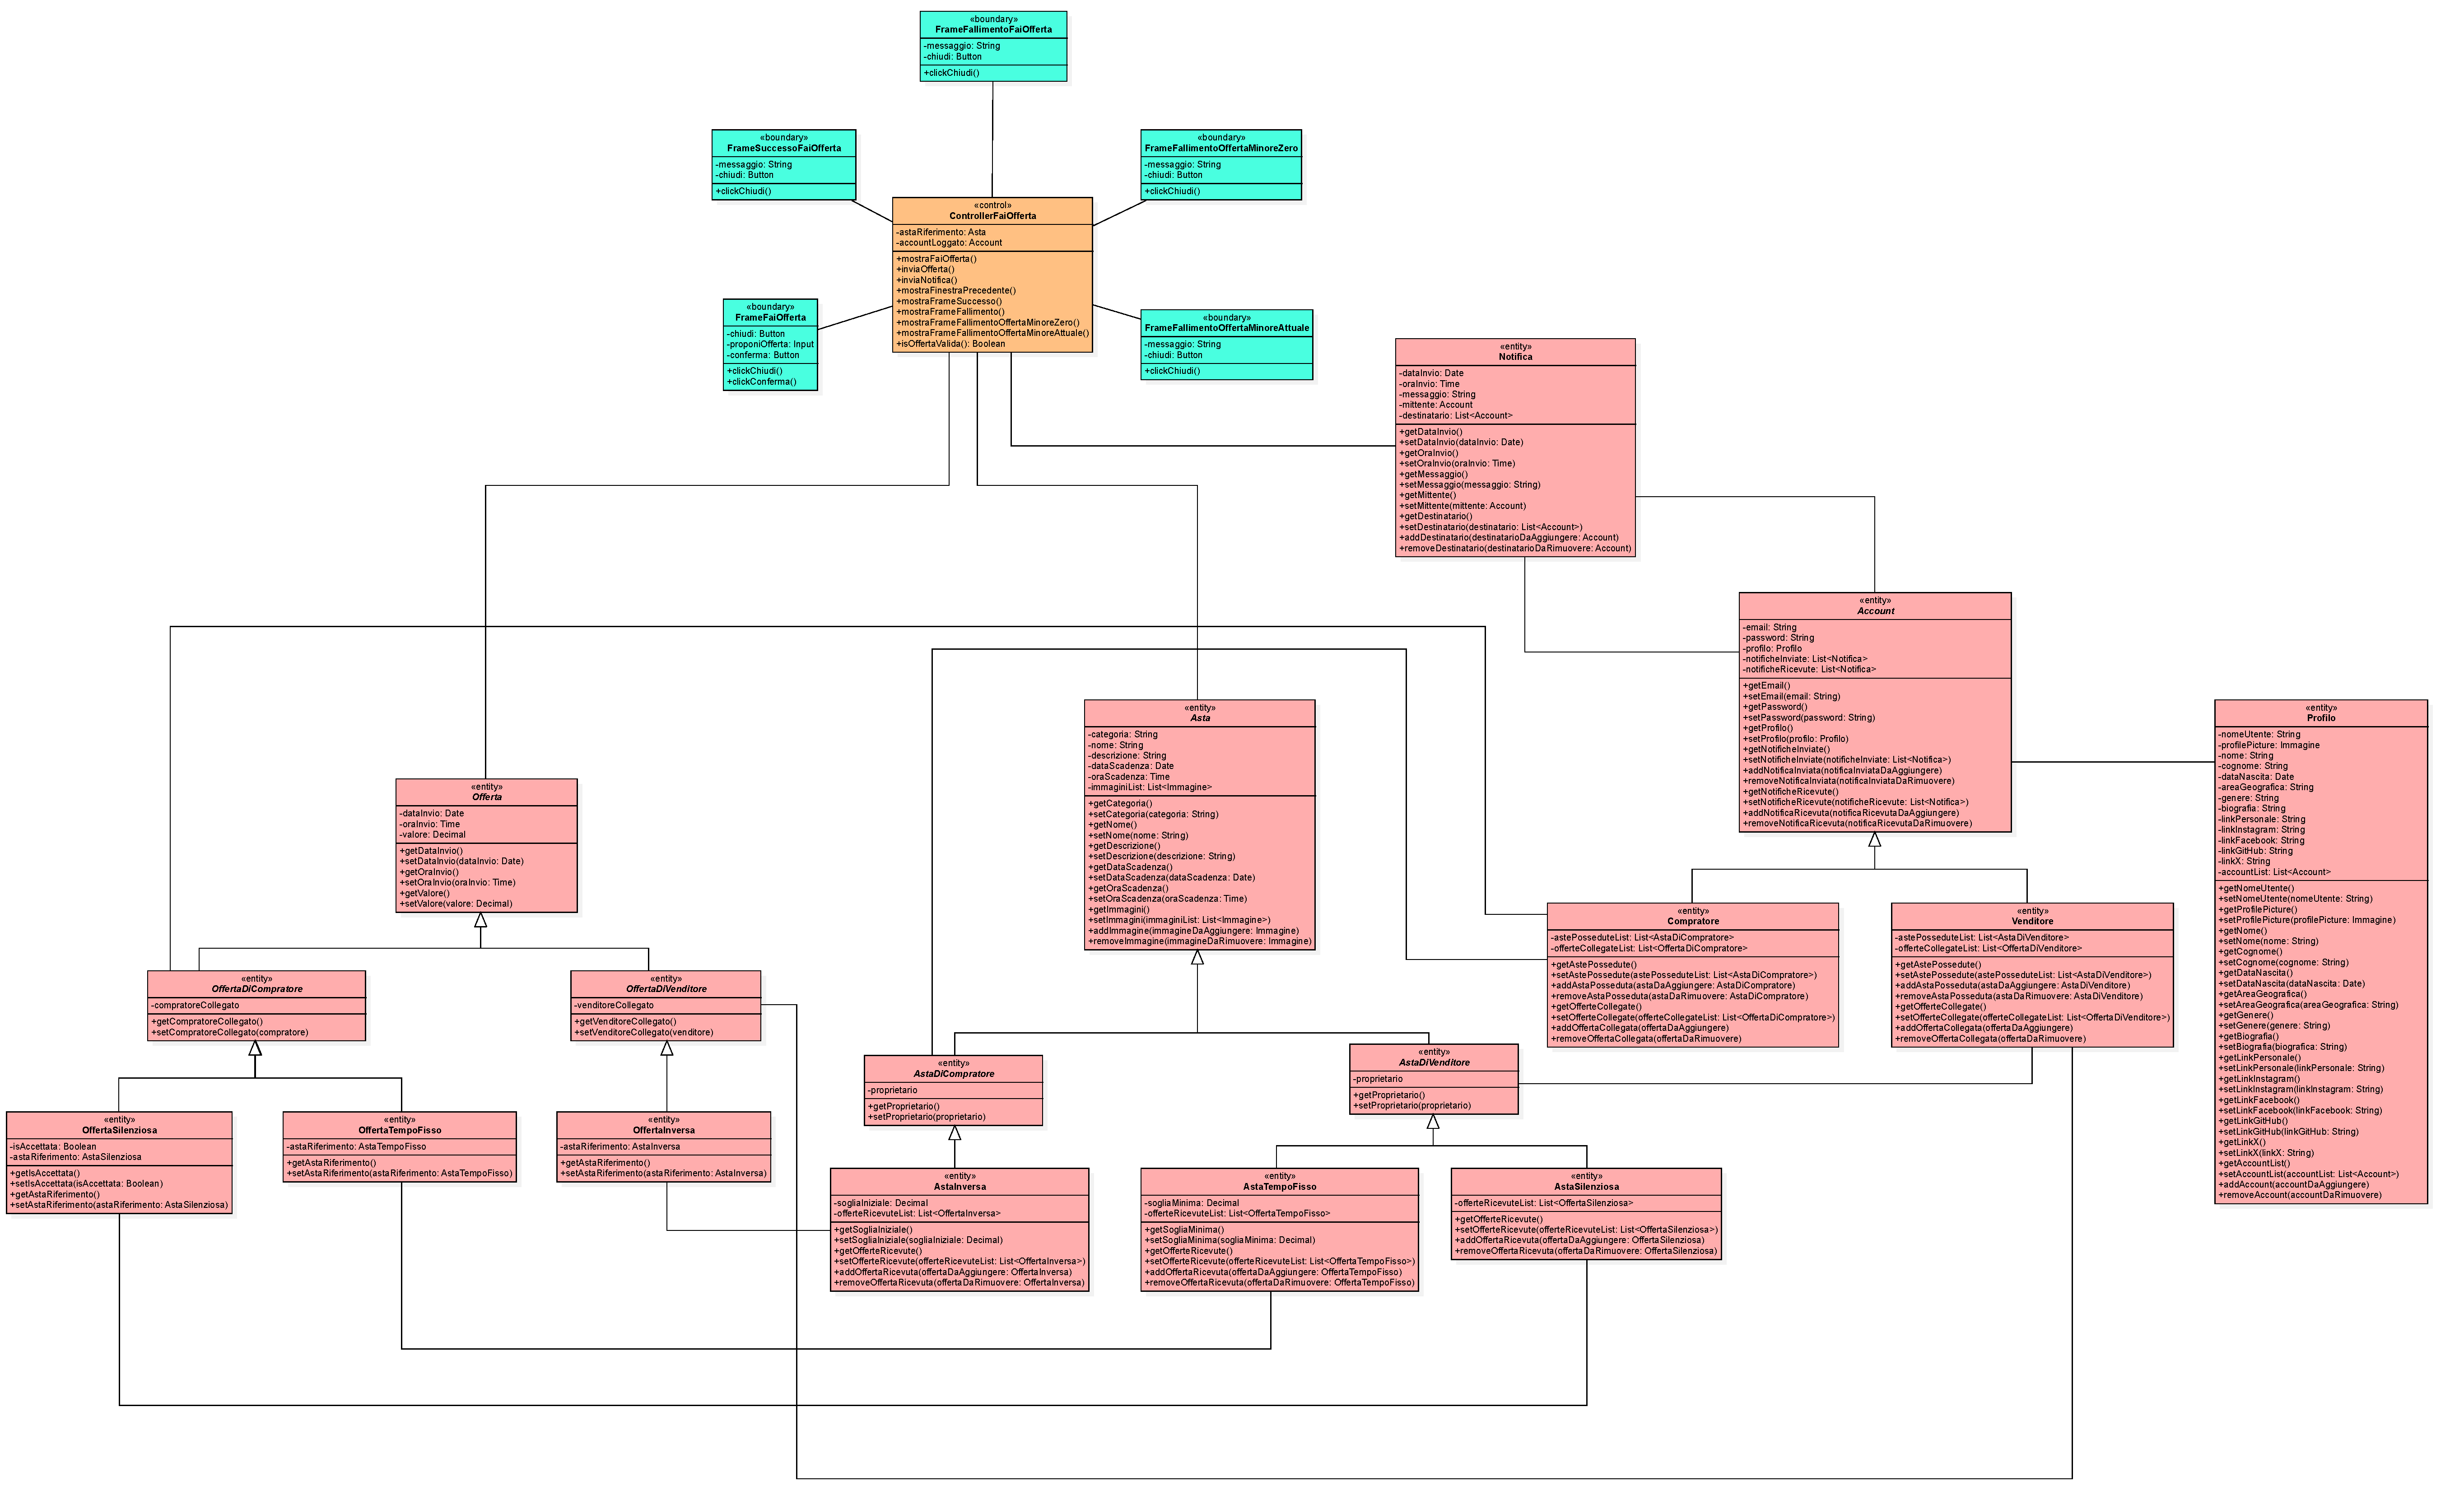
\includegraphics[width=1\linewidth]{Immagini/Diagrammi/Class Diagram/Venditore e compratore/FaiOfferta.pdf}
                \caption{Fai un'offerta}
            \end{figure}

    \clearpage
        
    \section{Dizionario delle classi}
        \begin{tabular}{|C{3.5cm}|L{11.2cm}|}
            \hline
            \multicolumn{1}{|c|}{\textbf{Classe}} & \multicolumn{1}{c|}{\textbf{Descrizione}}\\  
            \hline
                Account &
                Cosa rappresenta la classe\\
            \hline
                Venditore &
                Cosa rappresenta la classe\\
            \hline
                Compratore &
                Cosa rappresenta la classe\\
            \hline
                Profilo &
                Cosa rappresenta la classe\\
            \hline
                Notifica &
                Cosa rappresenta la classe\\
            \hline
                Asta &
                Cosa rappresenta la classe\\
            \hline
                Asta di compratore &
                Cosa rappresenta la classe\\
            \hline
                Asta di venditore &
                Cosa rappresenta la classe\\
            \hline
                Asta a tempo fisso &
                Cosa rappresenta la classe\\
            \hline
                Asta silenziosa &
                Cosa rappresenta la classe\\
            \hline
                Asta inversa &
                Cosa rappresenta la classe\\
            \hline
                Offerta &
                Cosa rappresenta la classe\\
            \hline
                Offerta di compratore &
                Cosa rappresenta la classe\\
            \hline
                Offerta di venditore &
                Cosa rappresenta la classe\\
            \hline
                Offerta a tempo fisso &
                Cosa rappresenta la classe\\
            \hline
                Offerta silenziosa &
                Cosa rappresenta la classe\\
            \hline
                Offerta inversa &
                Cosa rappresenta la classe\\
            \hline
        \end{tabular}
        
    \section{Dizionario delle associazioni}
        \begin{tabular}{|C{3.5cm}|L{11.2cm}|}
            \hline
                \multicolumn{1}{|c|}{\textbf{Associazione}} &
                \multicolumn{1}{c|}{\textbf{Descrizione}}\\            
            \hline
                Mittente &
                Cosa rappresenta l'associazione\\
            \hline
                Destinatario &
                Cosa rappresenta l'associazione\\
            \hline
                Possiede &
                Cosa rappresenta l'associazione\\
            \hline
                È associata a &
                Cosa rappresenta l'associazione\\
            \hline
                Possiede &
                Cosa rappresenta l'associazione\\
            \hline
                È collegato a &
                Cosa rappresenta l'associazione\\
            \hline
                Possiede &
                Cosa rappresenta l'associazione\\
            \hline
                È collegato a &
                Cosa rappresenta l'associazione\\
            \hline
                Si riferisce a &
                Cosa rappresenta l'associazione\\
            \hline
                Si riferisce a &
                Cosa rappresenta l'associazione\\
            \hline
                Si riferisce a &
                Cosa rappresenta l'associazione\\
            \hline
        \end{tabular}

    \section{Sequence Diagram}
        Il diagramma di sequenza rappresenta i processi e gli oggetti coinvolti e la sequenza dei messaggi scambiati necessari per adempiere ad una funzionalità. \\
        Le interazioni sono disposte lungo un'asse temporale per dare un'idea dell'ordine di avvicendamento dei messaggi.
        
        \begin{figure}[htbp!]
        \centering
            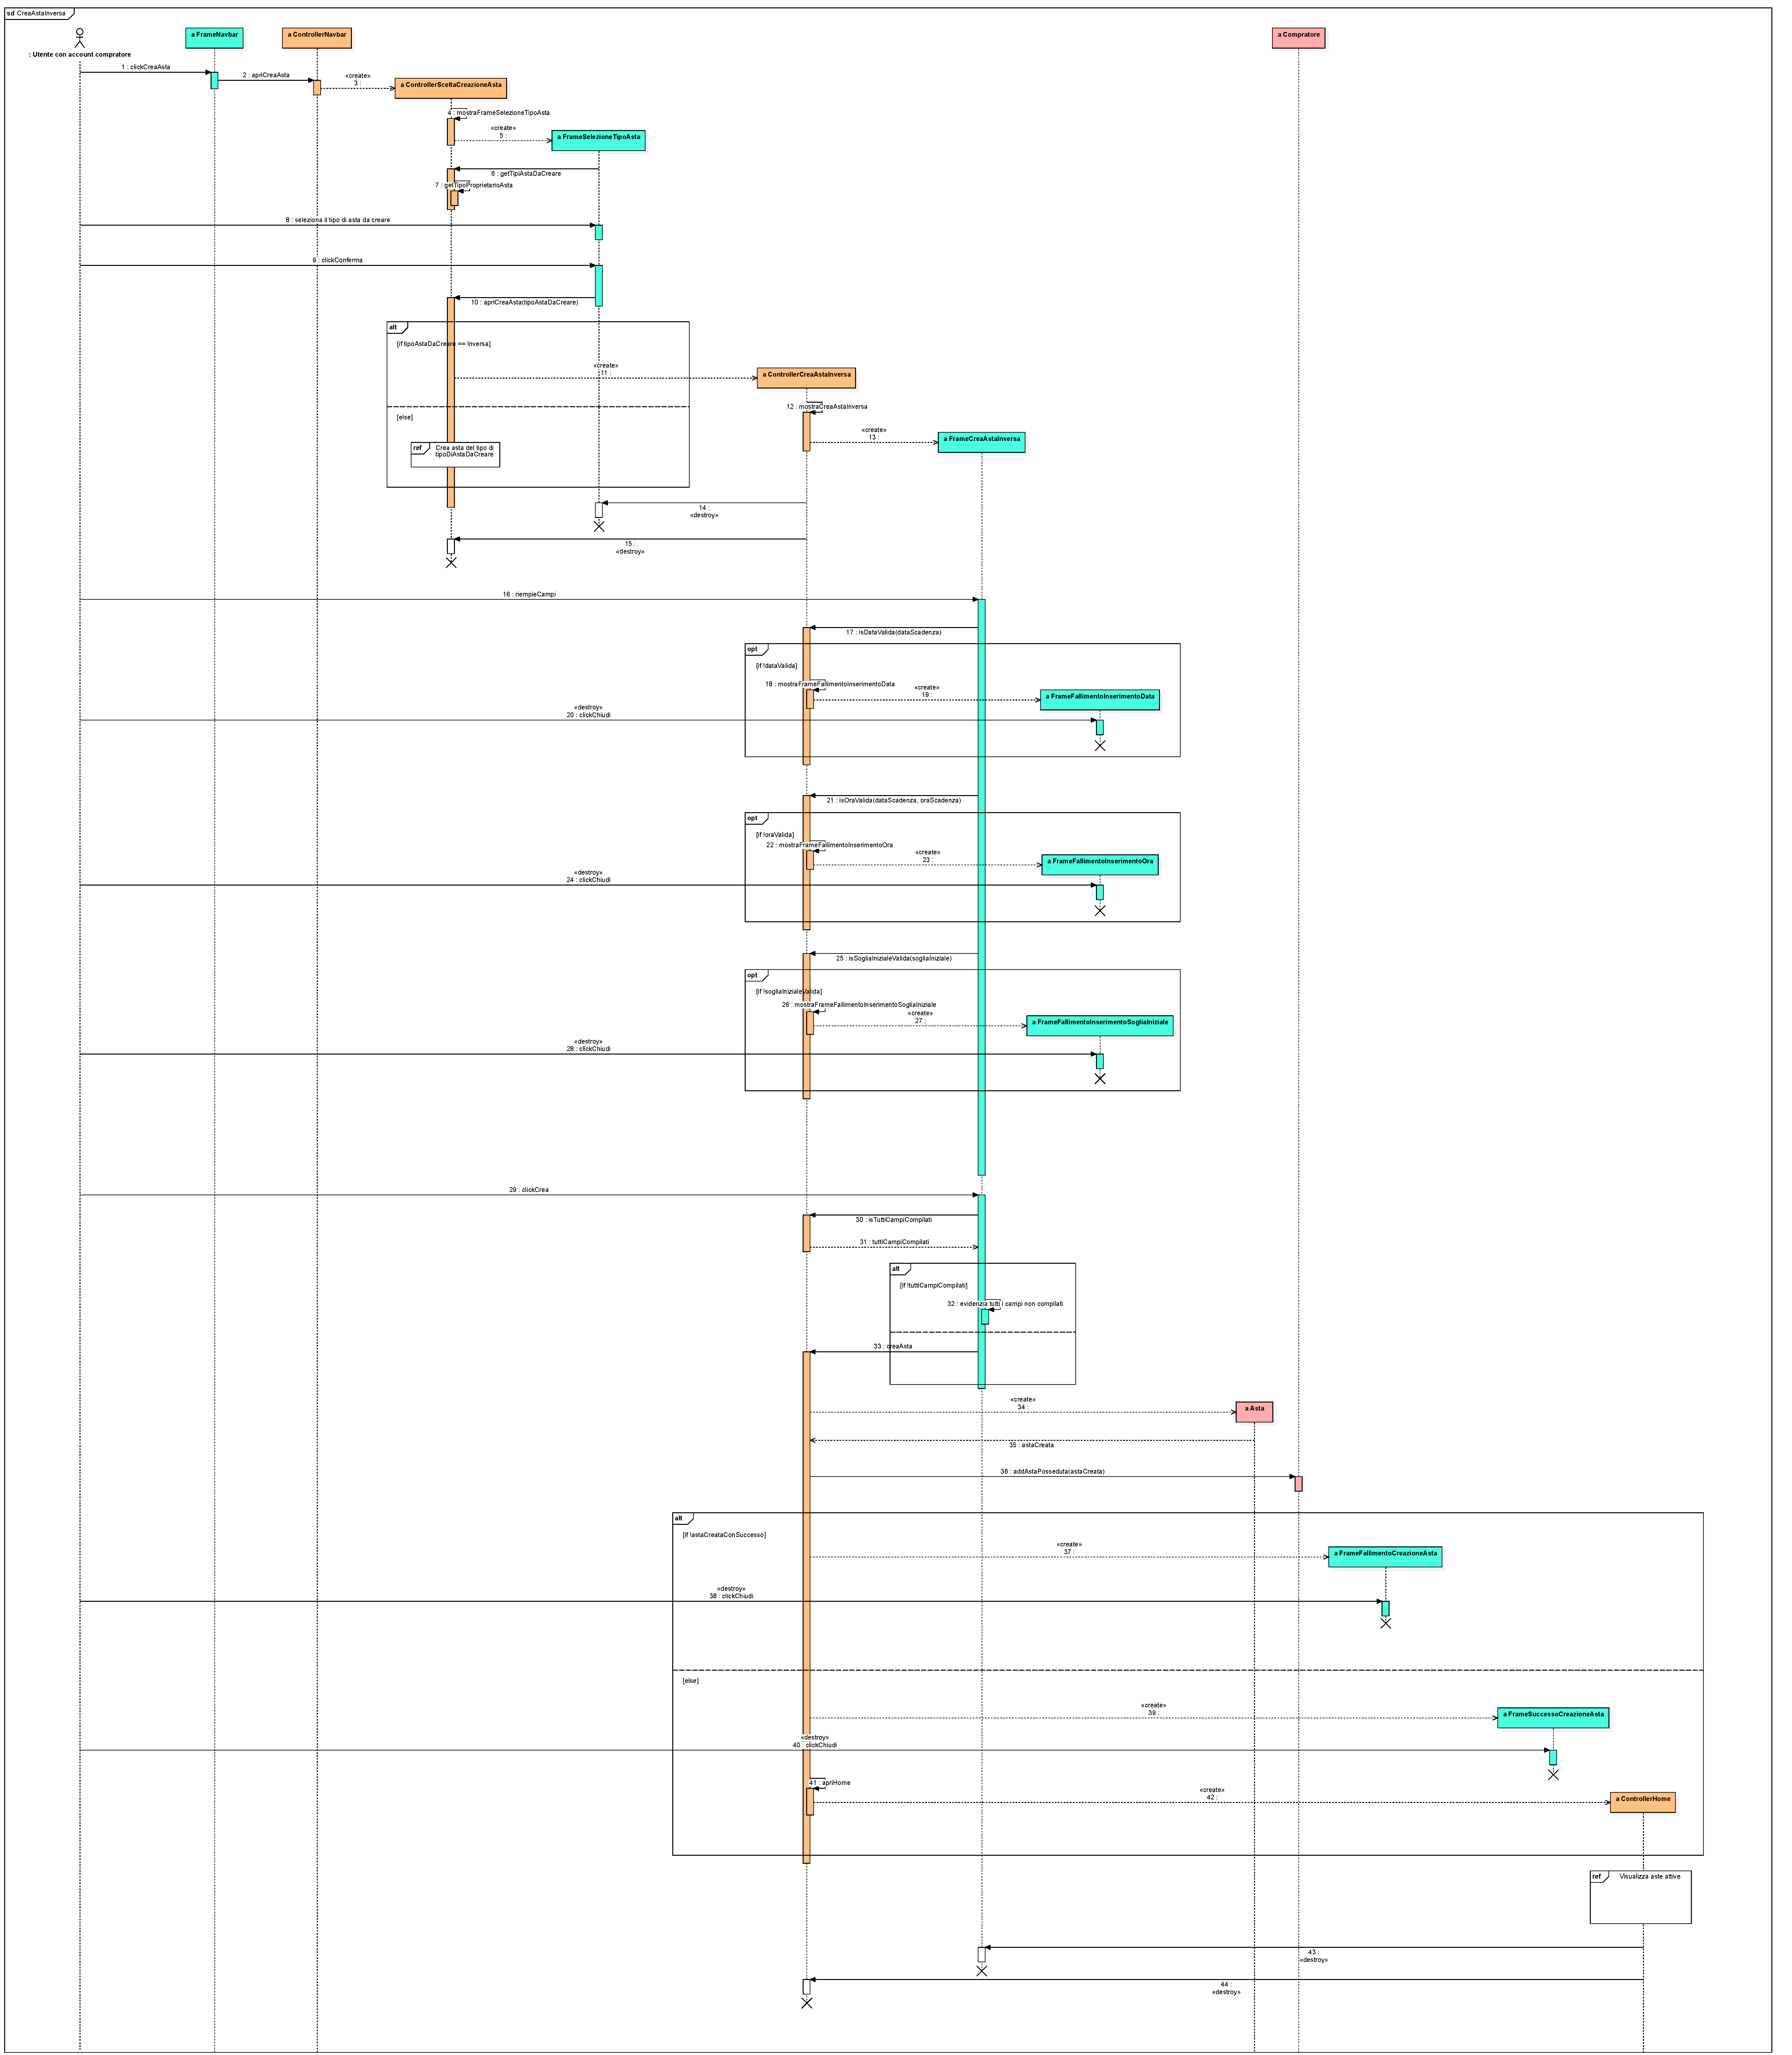
\includegraphics[width=1\linewidth]{Immagini/Diagrammi/Sequence Diagram/CreaAstaInversa.pdf}
        \caption{Sequence Diagram creazione asta inversa}
        \end{figure}

        \begin{figure}[htbp!]
        \centering
            \includegraphics[width=1\linewidth]{Immagini/Diagrammi/Sequence Diagram/AccettaOffertaSilenziosa.pdf}
        \caption{Sequence Diagram accetta offerta per un'asta silenziosa}
        \end{figure}

    \clearpage
    
    \section{Statechart Diagram}
        Il diagramma degli stati consente di rappresentare gli aspetti dinamici di un sistema, in particolare per l'interfaccia utente. \\
        Presenta quindi una serie di stati che il sistema attraversa (come una macchina a stati finiti), le azioni che comportano una transizione da uno stato all'altro, e le condizioni da rispettare affinché la transizione possa avvenire.

            \begin{figure}[htbp!]
            \centering
                \includegraphics[width=1\linewidth]{Immagini/Diagrammi/Statechart Diagram/CreaAstaInversa.pdf}
            \caption{Statechart Diagram creazione asta inversa}
            \end{figure}
            
            \begin{figure}[htbp!]
            \centering
                \includegraphics[width=1\linewidth]{Immagini/Diagrammi/Statechart Diagram/AccettaOffertaSilenziosa.pdf}
            \caption{Statechart Diagram accetta offerta per un'asta silenziosa}
            \end{figure}